\documentclass[doctype=phd,lang=en,bibstyle=apa]{ulthesis}

\usepackage{mystyle}

% Cover content
\department {Departamento de Informática}
\title      {Semantic Similarity Across\\Biomedical Ontologies}
\programme  {Doutoramento em Informática}
\branch     {Especialidade Bioinformática}
\author     {João Diogo Silva Ferreira}
\advisor    {Prof. Dr. Francisco José Moreira Couto}
\date       {2016}

% References
%\addbibresource{content/references.bib}
\addbibresource{content/references-mendeley.bib}

% During typesetting we might be interested in one chapter at a time
% \includeonly{
%     frontmatter/dedicatory,
%     frontmatter/acknowledgements,
%     content/00-abstract-pt,
%     content/00-abstract-en,
%     content/01-introduction,
%     content/02-concepts,
%     content/03-state-of-the-art,
%     content/04-validation,
%     content/05-enhancements,
%     content/05a-interlude,
%     content/06-data-description,
%     content/07-multidomain,
%     content/08-technical,
%     content/09-conclusions,
%     content/appendix-a,
%     content/appendix-b,
% }


% Start document
\begin{document}

\setcounter{page}{-6}
\pagenumbering{gobble}

\coverpage

\thispagestyle{empty}
\null

\begingroup
\parindent=0pt
\parfillskip=0pt

\small\slshape

% \setbox1=\hbox to 8cm{\hfil To my future children!}

\setbox0=\vbox{
    \setSpacing{1.15}%
    \frenchspacing
    \hsize=8cm
    \parshape=11
     0.00000pt 240.00000pt
     7.06669pt 225.86661pt
    14.13339pt 211.73323pt
    21.20008pt 197.59985pt
    28.26677pt 183.46646pt
    35.33346pt 169.33308pt
    42.40015pt 155.19969pt
    49.46685pt 141.06630pt
    56.53354pt 126.93292pt
    63.60023pt 112.79954pt
    70.66692pt 98.66615pt
    I wish to dedicate this thesis not to the usual suspects (not my wife or parents, my friends or teachers) but to those who I have had my mind on for a long time, the ones who will benefit the most from scientific discovery and from the vast accomplishments achieved today.\break I dedicate it, rather, to the ones who will linger after us and so reap the benefits of our hard work.\break\hfil\break To my future children!
}

\vskip10em

\centering
\leavevmode\box0

\endgroup

\cleardoublepage
\pdfbookmark{Acknowledgements}{Acknowledgements}
\chapter*{Acknowledgements}

Foremost, I would like to express my gratitude to my advisor, Prof.~Dr~Francisco M.\ Couto, whose expertise and undeniably scientifically oriented mind added considerably to my PhD. I appreciate his vast horizons and skills in many scientific areas (\eg semantic similarity, biomedical ontologies, Bioinformatics in general, just to list the ones more closely related to my research efforts), and his assistance in the extensive periods where writing was the major undertaking of my work (particularly the several manuscripts we jointly submitted for publication, as well as this document). Most of all, I look up to his ``relaxed'' yet serious attitude towards research, which always positively surprised me. Sometimes, research feels like a herculean task that we need to carry out in order to see some results, but more often it looks like a small train ride where we simply appreciate the landscape of knowledge to which we ourselves contribute.

My PhD companions, which are no longer students but Doctors, also deserve my gratitude: in no particular order, I thank Ana Teixeira, Catia M. Machado, Catia Pesquita, Daniel Faria, Hugo Bastos and Tiago Grego, with whom I collaborated in some way or another, and whom I could always count on to tag along on a brainstorming session over coffee. A further acknowledgement goes to André Lamúrias, with whom I collaborated towards the end of my PhD.

I recognize that this research would not have been possible without the financial assistance of the Fundação para a Ciência e Tecnologia, and express my gratitude to that agency for funding my PhD scholarship SFRH\slash BD\slash 69345\slash 2010.

I would also like to thank my parents for the infinite support they have been providing throughout my entire life, from the very first breath I took. The excellent upbringing you provided was the exact amount of motivation I needed to pursue the career in science that I now so dearly esteem. Thank you for always being there for me, for always helping me succeed. I also want to thank my brothers, André and Simão, for no other motive than that you are always present in my life. You are the best.

In particular, I must acknowledge my wife and best friend, Sandra, who stood by me every step of the way, who had to endure my absence whenever I needed to attend some conference, and without whose love, encouragement and unconditional assistance I would not have been able to finish this work. The biggest of my smiles is yours.

\vfill

{\flushright
\textit{Lisboa}, January 6\textsuperscript{th}, 2016\break
João Ferreira
\par}


% Start numbering pages with Roman numerals
\frontmatter

% Abstracts in several languages
\startabstract[pt]\cleardoublepage
\pdfbookmark{Resumo}{Resumo}
\begin{abstract}

\catcode`\_\active
\def_{\discretionary{-}{-}{-}}
\frenchspacing

As práticas que levam à descoberta científica estão geralmente associadas à necessidade de comparar entidades relevantes para essa mesma descoberta. Por exemplo, em medicina a comparação de um novo caso clínico com uma base de dados de casos antigos pode ajudar uma equipa médica a acelerar o processo de diagnóstico ou mesmo de tratamento; em investigação laboratorial, a semelhança na estrutura molecular de compostos químicos é útil na pesquisa de novos fármacos.

Apesar da necessidade de comparar as entidades anteriormente exemplificadas, é difícil encontrar métodos automáticos que sejam reprodutíveis, generalizáveis, e que consigam lidar com a diversidade destes dados. Na verdade, qualquer método automático tem obrigatoriamente de se basear numa representação objetiva e computacionalmente tratável dos dados, \eg objetos matemáticos como vetores ou sequências de caracteres. No entanto, a comparação de tais objetos é independente do contexto, \ie estes algoritmos de comparação transformam os dados sem qualquer conhecimento do seu significado. Além disso, este tipo de representação elimina por vezes informação relevante acerca das entidades. Exemplos de soluções pontuais para alguns tipos de dados incluem:
\begin{itemize}
    \item Comparação de compostos químicos através da sua estrutura molecular representada através de um grafo, onde os nós representam átomos e os arcos representam ligações químicas. Esta comparação pressupõe que uma semelhança na estrutura implica uma semelhança na atividade química dos compostos, uma relação que nem sempre é válida.
    \item Comparação de proteínas através da sua sequência de aminoácidos, o que como anteriormente nem sempre é válido uma vez que sequências parecidas não correspondem sempre a funções parecidas.
\end{itemize}

Por outro lado, há entidades que não são trivialmente representadas de forma matemática. Por exemplo, como comparar dois casos clínicos? Uma das formas de ultrapassar esta dificuldade é representar o próprio \emph{significado} num formato que possa ser interpretado por computadores, uma prática conhecida como representação do conhecimento.

A representação do conhecimento é uma área de investigação que tem como objetivo definir formas de tornar o conhecimento manipulável por computadores, tal como é manipulado por seres humanos, o que permite aplicar sobre ele algoritmos de raciocínio automático. O princípio mais útil desta área para o meu trabalho é que o conhecimento pode ser representado sob a forma de \emph{ontologias}, que são definidas, de forma simplista, como um conjunto
\begin{paralist}
    \item de conceitos relativos a um domínio do conhecimento, e
    \item das relações entre eles.
\end{paralist}
Por exemplo, uma ontologia que representa conhecimento anatómico define que \term{Coração} é um tipo de \term{Órgão}, e que \term{Fémur} é um \term{Osso} que \prop{articula_com} a \term{Tíbia}. As ontologias fornecem assim um \emph{significado} aos conceitos, não de forma explícita (como acontece por exemplo num dicionário, onde o significado é descrito em texto), mas de uma forma implícita, que emerge das relações definidas entre eles.

As ontologias permitem quantificar objetivamente o grau de semelhança entre os conceitos nelas contidos, através da comparação dos seus significados. Esta prática, conhecida como \emph{semelhança semântica}, permite determinar, por exemplo, que \term{Braço} é mais semelhante a~\term{Perna} do que a~\term{Coração}, uma vez que \term{Braço} e~\term{Perna} representam tipos de~\term{Membro}, enquanto que \term{Braço} e~\term{Coração} partilham entre eles apenas o conceito genérico~\term{Parte do corpo}.

Além da comparação entre conceitos, as ontologias permitem a comparação de entidades que estejam \emph{anotadas} com esses conceitos. No contexto deste documento, anotar uma entidade consiste em associar a essa entidade informação computacionalmente tratável que a descreva, geralmente através de conceitos de ontologias. Uma anotação não é mais do que uma descrição objetiva de um facto: ``esta entidade está relacionada com este conceito''. Por exemplo, é prática comum anotar as proteínas de uma base de dados com conceitos que representam as suas funções. Ao comparar as anotações de duas proteínas estamos efetivamente a comparar as duas proteínas; torna_se assim possível utilizar o próprio significado biológico das proteínas para as comparar, não sendo necessário recorrer a representações mais simplistas, como a sequência de aminoácidos.

Um dos aspetos da prática de semelhança semântica pouco investigados até ao momento é a questão da multidisciplinaridade dos dados. Em particular, na informática biomédica, os dados existentes são geralmente descritos com recurso a múltiplos domínios de conhecimento. Por exemplo, um caso clínico pode estar anotado com conceitos relativos aos sintomas, aos resultados de análises ao sangue, aos medicamentos prescritos, ou até a conceitos menos óbvios como os locais anteriormente visitados pelo paciente ou as suas condições sócio_económicas. Todos estes aspetos podem influenciar o diagnóstico e o tratamento escolhido, sendo portanto essenciais para um cálculo preciso da semelhança entre casos clínicos.

Este documento reporta a minha investigação na área da semelhança semântica no que respeita à sua aplicação em contexto multidisciplinar. Até à data, não existem trabalhos científicos publicados neste campo de investigação, sendo este o primeiro a surgir, não só na comunidade da informática biomédica como também no resto da comunidade científica. Eu proponho duas abordagens para comparar entidades multidisciplinares:
\begin{enumerate}
    \item Na abordagem \emph{agregativa}, todos os domínios de anotação são usados de forma isolada uns dos outros para calcular vários valores de semelhança unidisciplinar com um algoritmo pré_existente (\eg os sintomas de um caso clínico são comparados com os sintomas do outro caso clínico, depois os medicamentos de um caso com os medicamentos do outro, depois as condições sócio-económicas, \etc.). Os valores são por fim agregados matematicamente, \eg através da média.
    \item Na abordagem \emph{integrativa}, todas as ontologias relevantes são unificadas numa grande ontologia multidisciplinar, sendo em seguida aplicado um algoritmo de semelhança semântica pré_existente para comparar o conjunto de todas as anotações de uma entidade com o conjunto de todas as anotações da outra entidade.
\end{enumerate}

Ambas as abordagens se baseiam na existência de um algoritmo capaz de comparar dois conjuntos de conceitos provenientes de uma só ontologia (\emph{algoritmo de ontologia única}). Esta escolha baseia_se no facto de já existirem várias medidas capazes de executar essa tarefa, amplamente estudadas e aplicadas em vários casos. Além disso, as duas abordagens propostas são independentes da medida pré_existente utilizada, sendo portanto possível utilizar uma medida apropriada para o contexto em questão.

A metodologia seguida para provar que as medidas de semelhança multidisciplinar são eficazes no seu objetivo consistiu essencialmente em cinco passos:
\begin{enumerate}
    \item recolher dados multidisciplinares;\label{resumo:data}
    \item validar as duas abordagens acima descritas aplicando_as aos dados recolhidos;\label{resumo:multi}
    \item sistematizar os métodos de validação de semelhança semântica;\label{resumo:hierarchy}
    \item propor melhorias às medidas de semelhança de ontologia única; e\label{resumo:enhancements}
    \item criar \emph{software} para calcular a semelhança semântica de forma reprodutível.\label{resumo:software}
\end{enumerate}

Ao longo do meu doutoramento, recolhi três conjuntos de dados multidisciplinares anotados com conceitos de várias ontologias (passo~\ref{resumo:data}):
\begin{paralist}
    \item um conjunto de artigos científicos da área da epidemiologia anotados com conceitos como doenças, sintomas, vacinas, modos de transmissão, \etc.;
    \item um conjunto de vias metabólicas anotadas com compostos químicos, enzimas, doenças associadas a erros na via metabólica e drogas que afetam o funcionamento das vias; e
    \item um conjunto de modelos matemáticos de sistemas biológicos, anotados com compostos químicos, enzimas, entidades anatómicas e fenótipos.
\end{paralist}

Para validar as abordagens multidisciplinares (passo~\ref{resumo:multi}), segui três estratégias de validação distintas:
\begin{paralist}
    \item prever novas anotações com base nas já existentes,
    \item classificar automaticamente os dados com base nas suas anotações, e
    \item comparar os valores de semelhança obtidos automaticamente com valores de semelhança atribuídos manualmente por especialistas.
\end{paralist}
Em cada uma destas estratégias, calculei uma métrica de desempenho que permite determinar a validade das medidas de semelhança semântica.

Os resultados obtidos com as três estratégias de validação mostram empiricamente que as medidas de semelhança multidisciplinares são de facto eficazes. Por comparação do desempenho atingido por cada abordagens multidisciplinar (agregativa e integrativa), conclui_se que a abordagem integrativa é em geral superior à abordagem agregativa. Este resultado corresponde ao que era esperado, uma vez que a abordagem integrativa tem acesso a mais informação, pois utiliza relações existentes entre conceitos de duas ontologias diferentes e portanto atinge valores de semelhança mais precisos.

Comparei ainda o desempenho das abordagens multidisciplinares com o desempenho obtido com as medidas de semelhança de ontologia única. Apenas em alguns casos excecionais as abordagens multidisciplinares não foram superiores às medidas de ontologia única (esta situação ocorre essencialmente quando se utilizam anotações de uma ontologia que já representa, por si mesma, vários domínios de conhecimento, e portanto a adição de novos domínios de anotação não melhora o resultado).

Outras contribuições importantes foram atingidas com este trabalho. Nomeadamente:
\begin{itemize}
    \item Estabeleci uma hierarquia de estratégias de validação para utilizar no desenvolvimento de semelhança semântica, a qual permite organizar os vários métodos de acordo com o tipo de aplicações onde podem ser usados (passo~\ref{resumo:hierarchy}).
    \item Propus novas medidas de semelhança de ontologia única que exploram uma maior quantidade da informação representada nas ontologias, aumentando não só o leque de algoritmos disponíveis mas também o seu desempenho (passo~\ref{resumo:enhancements}).
    \item Desenvolvi uma infraestrutura de \emph{software} que permite obter resultados de semelhança semântica não só de forma rápida mas reprodutível, sendo extensível, ou seja, permite que outros investigadores facilmente implementem os seus algoritmos de semelhança semântica (passo~\ref{resumo:software}).
\end{itemize}

Com o aumento da quantidade de conhecimento que nós humanos vamos construindo e ao qual vamos tendo acesso, é a simbiose entre investigadores e métodos automáticos que permite gerir o conhecimento de forma eficiente. Só assim poderemos, como comunidade, garantir a descoberta de nova informação e assegurar que ela pode ser utilizada no futuro. A semelhança semântica é apenas um dos aspetos desta automatização.

A minha contribuição, como quase todas em ciência, permite vislumbrar apenas um pouco além da fronteira que engloba o conhecimento humano, mas juntamente com as descobertas de milhões de outros cientistas, está a construir e a melhorar o conhecimento que temos do nosso mundo e de nós próprios. Assim, considero que o meu trabalho é um pequeno mas robusto passo em direção ao futuro da Ciência.


\begin{keywords}
    Semelhança semântica multidisciplinar,
    Ontologias biomédicas,
    Anotação de entidades biomédicas,
    Web Ontology Language,
    Web semântica,
    Validação de semelhança semântica,
    Multidisciplinaridade dos dados biomédicos
\end{keywords}

\end{abstract}

\startabstract[en]\cleardoublepage
\pdfbookmark{Abstract}{Abstract}
\begin{abstract}

The need to compare complex entities is relevant in all the areas of science. In medicine, for example, comparing a clinical case to a database of previous cases can be extremely helpful when trying to diagnose a disease or deciding the most appropriate treatment for a patient.

% ; in journalism, in particular online journalism, comparing news can be used
% to track user preferences which, in turn, can help select information to be
% presented on the screen based on its relevance to the user.

Recent developments in knowledge representation, in particular the creation of the Web Ontology Language (OWL), have lead to a rise in the amount of knowledge that is being stored in \emph{ontologies}, which represent, in machine-readable format, the known facts about reality. With the help of ontologies, statements like ``\term{Influenza} is an \term{Infectious disease}'' can be processed by computers, which, in turn, can be used to create new knowledge. In particular, \emph{semantic similarity} has emerged to explore these ontologies as a way to compare entities annotated with the ontology concepts.

% Because it is known that \term{Arms} are \term{Limbs} and that \term{Legs} are also \term{Limbs}, it can be assessed that the similarity between \term{Arm} and \term{Leg} is higher than the similarity between \term{Arm} and, e.g.~\term{Head}.

Semantic similarity has been extensively studied in the last decade, but some problems still persist. While there are algorithms to compare entities annotated with concepts from the same ontology, the possible ways to use \emph{more than one ontology} are still in an early phase of study. For example, comparing a metabolic pathway using both the associated molecular functions and the metabolites converted in the pathway should, in principle, yield a higher precision than would be achieved with methodologies that rely on either one of the two domains independently. Comparing concepts from \emph{different domains} and entities annotated with concepts from different domains is yet an unexplored area, but necessary to tackle multidisciplinary biomedical resources, \eg to compare two clinical cases, the relationships between symptoms, diseases, blood screening results, \etc.\ should provide a more insightful and precise value of similarity.

In this document, I explain the basic concepts needed to understand the problem of semantic similarity, how it is being solved, and how I propose to extend this notion so that it can be applied to more than one ontology and, more significantly, to more than one domain of knowledge.

\begin{keywords}
    Multi-domain semantic similarity,
    Biomedical ontologies,
    Biomedical annotated entities,
    Web Ontology Language,
    Semantic web,
    Semantic similarity validation,
    Multidisciplinarity of biomedical data
\end{keywords}

\end{abstract}


% Lists in the front matter
\cleardoublepage
\tableofcontents*
{\def\mathversion#1{}\cleardoublepage\listoffigures}
{\def\textbf{}\cleardoublepage\listoftables}
\cleardoublepage\listoflistings

% \cleardoublepage\listoftodos

% Switch to Arabic numeration
\mainmatter

\part{Background}
\epigraph{Imagination is the beginning of creation. You imagine what you desire, you will what you \penalty-500 imagine and at last you create what you will.}{George Bernard Shaw}

\chapter{Introduction} \label{chap:intro}

The process of finding similar and related concepts is one of the most characteristic activities of human nature and, specifically, of scientific research. Indeed, the categorisation of known concepts (\ie the proper distribution of the concepts in manageable categories, where each category contains only concepts that are similar to each other) introduces an abstraction layer over the reality that enables a more focussed reasoning over experimental results and empirical observations. The importance of categorisation is tightly coupled with the amount of concepts that one must deal with: as the amount of collective human knowledge increases, so does the needs for good categorisation that abstracts away the less useful details of reality, thereby increasing its manageability.

Therefore, similarity and relatedness measures are, without a doubt, necessary assets for the advancement of science. As we will see in this document, I argue that \emph{semantic} measures are, in fact, one of the most useful ways to achieve similarity and relatedness values for today's scientific resources, which are now sufficiently ripe for use in research, with particularly applicable results in the context of biomedical informatics.

The findings of this thesis focus primarily in the biomedical domain, given that the level of commitment in the biomedical informatics community to develop automatic systems to help their research (and ultimately contribute to the medical practice) is extremely high. For this reason, the whole document is written with a biomedical point of view. However, it is important to notice that the results that I will describe later and the contributions that stem from the work that I carried out can be generalised into other areas of research with minimal effort.


\section{Motivation} \label{sec:intro/motivation}

It is an undeniable and undisputed fact of scientific research that the amount of knowledge and data published each year is increasing at an exponential pace~\citep{Larsen2010}. This behaviour is true not only across areas of research but also across types of publication: it can be observed in the number of academic papers as well as in the sizes of databases, with staggering examples in protein databases \citep[\eg][]{Uniprot2010} or chemical databases~\citep{Williams2008}. Even clinical information can be collected (subject to ethic guidelines, given the need for confidentiality in such records) and used in research, a practice called translational medicine~\citep{Nalichowski2006,Wehling2008}. \figref{fig:medline-growth} illustrates this facet of scientific discovery by plotting the amount of articles contained in MEDLINE (a bibliographic database for the life sciences) against time, which shows an approximately exponential trend. The same behaviour can be observed in other databases of biomedical information, such as the one in \figref{fig:pdb-growth}.

\begin{figure}
    \centering
    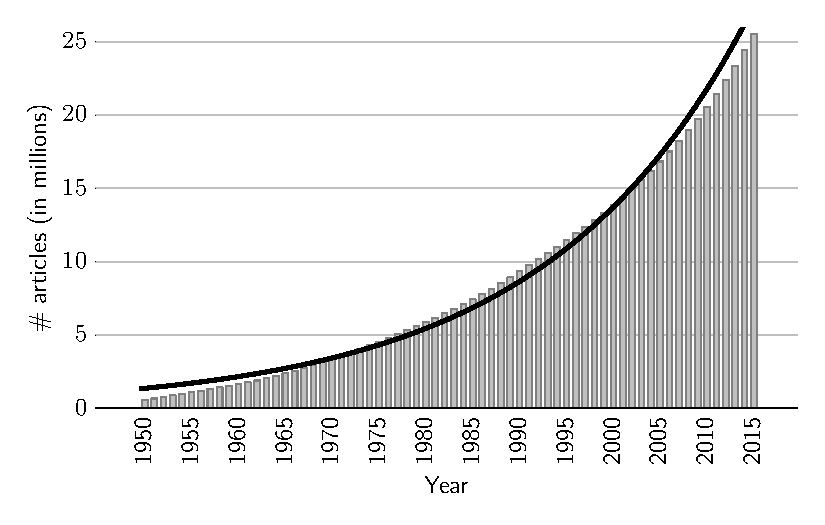
\includegraphics[width=0.8\textwidth]{images/medline-stats.pdf}
    \caption[Yearly size of MEDLINE from 1950 to~2015]{This plot shows that the number of bibliographic entries in MEDLINE has increased exponentially. The bars represent the cumulative number of articles indexed in this database each year, while the bold line is an exponential fit to the data. This rate of growth corresponds, on average, to a doubling in the amount of articles every $15.0$~years. Data retrieved from an actual search for publications between 1950 and~2015, in \url{http://www.ncbi.nlm.nih.gov/pubmed}. This image is meant as an illustration only, as there are many scientific results that are not published in MEDLINE-indexed journals.}
    \label{fig:medline-growth}
\end{figure}

\begin{figure}
    \centering
    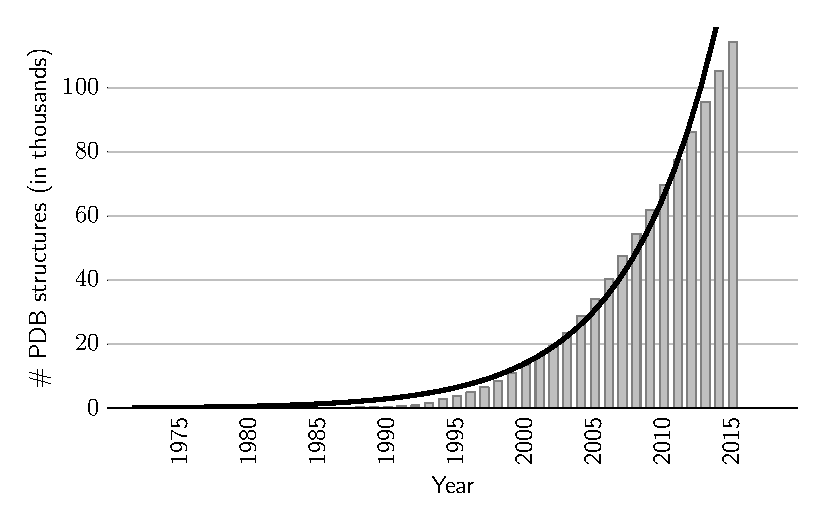
\includegraphics[width=0.8\textwidth]{images/pdb-stats.pdf}
    \caption[Number of $3$-dimensional protein structures in PDB from 1975 to~2015]{This plot shows that the number of protein structures stored in the Protein Data Bank has increased almost exponentially since the database has been created. The bars represent the total number of structures in this database, while the bold line is an exponential fit to the data. This rate of growth corresponds, on average, to a doubling in the size of the database every $4.5$~years. Data from \url{http://www.rcsb.org/pdb/statistics/contentGrowthChart.do?content=total}.}
    \label{fig:pdb-growth}
\end{figure}

   
With this exponential increase, two major problems have arisen. First, it has become impossible for researchers to fully read and interpret all the new information that becomes available each day. Second, and more important in scientific research, data published by different authors is often released in different formats, with different assumptions on what the meaning of each particular datum is. This makes it difficult, and in some cases impossible, to properly integrate all this information under a central knowledge repository without a lot of effort on the part of the data owners.

Surprisingly, these two problems are related, and solving one will help solve the other. Specifically, the impracticality of manually reading papers has created the need to develop automatic systems able to read textual documents, to appropriately parse and interpret them, and finally to draw conclusions based on them (for example by generating an automatic summary). To allow such a system to function, it must be able to understand the \emph{meaning} underlying the concepts referred to in the text, which, for example, includes understanding that the heart is responsible for pumping blood, that muscles are attached to bones through tendons, or that infections can cause fever. This, in turn, requires that knowledge be encoded in a machine-readable format, which must be precise, formal, and comprehensive, enabling computers to perform reasoning. Only that allows a computer to interpret text. On the other hand, knowledge that is described in such a format, using standard representations that everyone agrees with, can also be used by computers and, ultimately, be regarded as interoperable. This solves the second issue: if an automatic system is able to parse data from multiple sources in a logical format, it can use them uniformly as if they had the same provenance.

There are, today, many organisations dedicated to the production of formal standards for knowledge representation as well as \emph{reference knowledge artefacts} (called ontologies throughout this document), predominantly in the biomedical informatics community. For example, the Gene Ontology (\ontology{GO}), first published in 2000~\citep{Ashburner2000}, is an attempt to ``address the need for consistent descriptions of gene products in different databases''~\citep{GOIntroduction}. With the maturation of the standards for knowledge representation and the semantic web (see \secref{sec:concepts/knowledge-representation,sec:concepts/ontologies,sec:concepts/semantic-web} for a summary of the importance of these concepts to the field of biomedical informatics), \ontology{GO} has grown into a mature digital artefact that represents properties of proteins such as molecular function and cellular localization.

To explore the wealth of information that is stored in biomedical data, it is vital that ontology developers and users be provided with tools that can properly manage and handle the data; one ubiquitous requirement in science is the ability to estimate the degree of similarity or relatedness between the various ontology concepts~\citep{Vision2011} and, by extension, between multidisciplinary entities. For instance, similarity between proteins is often associated with one or more functions being shared among them~\citep{Altschul1990}; in chemistry, similarity of molecular structure correlates with similar biological role~\citep{Hansch1964,Klebe1994}; in medicine, a high degree of similarity between two clinical cases is a strong argument towards a similar diagnosis~\citep{Swender1974}.

One of the technologies enabled by the use of ontologies is indeed the calculation of similarity between the concepts they represent, a technique known as ``semantic similarity''~\citep{Resnik1995,Lord2003,Pesquita2009}. This technique can be used to compare concepts within one ontology as well as entities annotated with those concepts. For example, proteins annotated with \ontology{GO} functions can be compared based on the semantic similarity of those functions. While traditional automatic systems compared proteins by their sequence, using methods such as BLAST~\citep{Altschul1997}, semantic annotations provide a mechanism to compare proteins by their functions~\citep{Lord2003}. Advantages of this include the fact that some proteins that are known to have similar functions have different sequences, or vice-versa. Thus, semantic similarity can explicitly explore information about entities (in this case proteins) to more accurately compare them.

Semantic similarity has been applied to various domains:
\begin{itemize}
    \item between proteins annotated with \ontology{GO} concepts describing their molecular functions~\citep{Lord2003,Lei2006};
    \item between metabolic pathways annotated with their enzymes~\citep{Clemente2005} or chemical compounds~\citep{Grego2010}; and
    \item between diseases annotated with biological processes~\citep{Schlicker2010}.
\end{itemize}
Real world problems whose solution incorporates semantic similarity include the prediction of
\begin{paralist}
    \item the probability of a certain disease given a set of symptoms~\citep{Kohler2009},
    \item the cellular localization of proteins given their annotations~\citep{Lei2006},
    \item the function of proteins~\citep{Pesquita2008}, and
    \item the chemical properties of small metabolites~\citep{Ferreira2010}.
\end{paralist}

One of the remaining issues in this area is related to the fact that ontologies are often developed with a single domain of reality in mind. \ontology{GO} represents knowledge associated with proteins, \ontology{CHEBI} (Chemical Entities of Biological Interest) represents knowledge associated with biologically relevant chemical substances~\citep{Degtyarenko2008a}, \ontology{FMA} (Foundational Model of Anatomy) represents human anatomy~\citep{Rosse2003}, \etc. But knowledge is multidisciplinary, with some concepts from one domain being often intertwined with concepts from another domain. This is particularly true in the biomedical field, which is so vast that it is partitioned in several distinct but related disciplines. Clinical cases, for example, may include information on the symptoms, blood screen results, and drugs the patient is currently taking; even less obvious concepts, such as the previously visited places and the economical conditions of the patient can prove useful in tracing a diagnostic. Models of metabolic pathways refer to the reactions, the enzymes, the chemical metabolites the cellular components involved in the pathway, \etc. When accuracy is necessary (and it frequently is in the biomedical domain), multidisciplinarity naturally arises.

While single-ontology semantic similarity has been extensively studied in the last two decades, current algorithms are unable to adequately compare multidisciplinary entities. To handle multidisciplinarity, I propose that it is possible to harness the advantages of the existing single-ontology measures to allow their use in this context, by \emph{lifting} them from the single-ontology constraints. For this purpose, I study the following two approaches:
\begin{enumerate}
    \item Use single-ontology measures to compare concepts from the same domain in the two entities with single-ontology measures (\ie compare the chemical reactions of one entity with the chemical reactions of the other entity, then cellular components with cellular components, symptoms with symptoms, \etc.)\ and then combine the various results in a single value by means of an aggregating function such as the average. I call this the \emph{aggregative} approach.
    \item Use the inherent expressiveness of ontologies to integrate all knowledge in a single multidisciplinary knowledge base. Instead of calculating a value for each domain, this approach exploits the inter-domain links that exist between the ontologies to calculate multi-domain similarity and relatedness. For example, the relationship between skin and rash can be used to link together an ontology of anatomy and one of symptoms. I call this the \emph{integrative} approach.
\end{enumerate}


\section{Objective} \label{sec:intro/objective}

The theoretical objective of my PhD was to prove the following thesis:

\begin{quote}
Multi-domain semantic similarity measures can be constructed by lifting single-ontology measures according to the two approaches defined above (the aggregative and integrative approach), thus enabling semantic similarity on multidisciplinary entities.
\end{quote}
This statement is the driving force behind all the research efforts related to my work. In particular, I expect
\begin{paralist}
    \item that the comparison of multidisciplinary entities will be more effective when using a multi-domain measure rather than a single-ontology measure applied only to one domain, and
    \item that the integrative approach will generally be more effective than the aggregative approach, as it has access to more information.
\end{paralist}

\emph{Effectiveness} is an abstract concept that can have several interpretations depending on the context in which it is applied. In a medical context, a measure is effective if it can, for example, predict a disease from the clinical notes associated with a patient; in pharmacology, a measure is effective if it can be used to diminish the costs of drug tests by pre-emptively filtering potential drugs, thereby reducing the number of necessary trials. The proposed hypothesis, however, is orthogonal to the measure of effectiveness that one uses: irrespective of the way effectiveness is calculated, multi-domain measures perform well.

% As far as I was able to ascertain, no previous work has been published that explores the idea of multi-domain semantic similarity (more information on current methodologies in this area will be discussed in \chpref{chap:sota}). As such, evaluating the developed work will be a non-trivial task and as such the assessment of the \emph{effectiveness} of my similarity measures will not be as comprehensive as could be desired. However, there has been a recent \emph{hype} in the development of single-domain semantic similarity measures \citep[\eg][]{Lord2003,Pesquita2008,Kohler2009}, and as such the utility factor of multi-domain similarity measures (their effectiveness) can be evaluated through a direct comparison of the two approaches defined in the motivation. Given the nature of biomedical ontologies, specifically the dependency that exists between them, I was able to develop an integrated platform of similarity to better reflect the true similarity of biomedical concepts.

The practical and more fundamental objective of this thesis is, therefore, the creation of both
\begin{paralist}
    \item a semantic similarity framework that is able to deal with multidisciplinary entities, and
    \item semantic similarity measures that quantify these entities in a way that reflects their actual meaning.
\end{paralist}
For the first part, I will develop a system that is able to use existing single-ontology measures and lift them to multi-domain measures. For the second part, the focus will fall on finding use cases where multi-domain semantic similarity is needed, such as the detection of similar biochemical pathways or similar epidemiological resources. These datasets will be used to evaluate the effectiveness of multi-domain measures.

% \margin{This paragraph is weird!}
% Since there are ontologies that contain concepts for diseases (\eg the Human Disease Ontology), it could be argued that a single-ontology similarity measure on that ontology should suffice when comparing diseases. However, to correctly describe a disease, more information should be used. For instance, information such as the fact that some people with the flu exhibit fever symptoms does not fit into an ontology, since it is non-universal (not everyone with fever has the flu and not everyone with the flu displays fever symptoms). Treatments can be useful when comparing diseases, but the relation between treatment and disease is also non-universal. Furthermore, other biomedical entities, such as clinical cases, do not belong into ontologies, and are better described with explicit links to concepts. In these cases, multi-domain similarity measures are the only way to fully explore the wealth of information contained in these descriptions.


\section{Methodology} \label{sec:intro/methodology}

To achieve the main objective of this thesis, I had to fulfil five separate tasks.

% \point{Test preliminary single-domain measures}
% As a preliminary work, I have explored current techniques for \emph{single-domain} semantic similarity measures. To this effect, I continued my previous work on the Chemical Entities of Biological Interest (\ontology{CHEBI})~\citep{Ferreira2010}, using semantic similarity and machine-learning approaches to predict chemical compound functions; assisted in the development of semantic similarity for Geo-Net-PT~\citep{Batista2012}, an ontology of geospatial locations in Portugal; and devised a semantic \emph{relatedness} measure for the Foundational Model of Anatomy (\ontology{FMA})~\citep{Ferreira2011}.

\point{Study how validation is done in the field of semantic similarity}
Biomedical research in this field has been generating innovative and useful measures of similarity since~2003 and applying them to several distinct problems; however, validation is still being done in a relatively \emph{ad hoc} way, where each proposed measure is validated with a different method without much relation to previous ones. While some steps have been followed to mitigate this problem, a true systematization of validation strategies is still lacking, and as such one of the tasks of my work will be to determine to what extent this problem can be alleviated.

\point{Enhance current similarity and relatedness measures}
With the recent advance in the research of knowledge representation, ontologies are becoming increasingly richer and more expressive, and tools are being developed to handle this expressiveness. However, semantic similarity is not following this trend. For example, most algorithms are agnostic to the ideas of formal axioms, and as such are unable to use facts like the ones expressed with disjoint axioms (\ie there is no thing that is both a \term{Square} and a \term{Circle}) or other logic axioms. I believe that exploring in more detail the formal logic aspect of ontologies will yield measures of similarity that better reflect the structure of the ontology and the relationships between its concepts.

% The application of algorithms of ontology alignment will also prove invaluable to this thesis, since they find links between two ontologies, which enables the use of the integrative approach to multi-domain semantic similarity. As explained earlier, multi-domain measures need the integration of the several ontologies used, and this is only possible if there is a set of known facts between these concepts (\eg the previosuly mentioned relation between \term{Skin} and \term{Rash}).

% Another point of interest in this task is the exploration of machine-learning for the selection of attributes that better represent the concepts being compared. For example, a semantic similarity measure between two epidemiological resources may be dependent on the location of surge being studied, or on the economic conditions of that place, but in the domain of general diseases, the location may not be as relevant. In order to study the effect of all the information involved in the description of the objects being compared, there has to be a notion of how important these attributes are, which can be estimated with machine-learning approaches. This may be a critical step for the aggregative approach, since the exact features used must be carefully selected to yield a reasonable and practical measure.

% Additionally, the notion of \emph{information content} (see \secref{sec:concepts/ssm,sec:sota/node}) has been proved useful in single-domain similarity measures. This concept will probably play a major role in the measures of similarity, since it quantifies the specificity of ontology concepts. Therefore, the correct exploration of a multi-domain information content measure will be subject of study as well.

\point{Collect multidisciplinary datasets}
To test the measures of similarity and relatedness developed in this thesis, it will be necessary to collect multidisciplinary data annotated with concepts from various ontologies, which will allow the use of the aggregative and integrative approaches. Another important aspect of this task is the possibility to use the data collected and the help of experts to create gold-standards that can be used to validate the measures of similarity.

\point{Validate the multi-domain measures}
This task will finalise the proof of the proposed thesis by finding evidence that supports it. Validation of multi-domain semantic similarity measures can be done in several ways. For example, by comparing the automatically assigned similarity values with the ones assigned by experts in the gold-standards created in the previous task, or by using it in classification problems and quantifying the difference in performance between the single-ontology measures and the multi-domain approaches.

\point{Develop semantic similarity software}
Given the increasing number of ontologies, the amount of multidisciplinary data being published, and the growing standardization efforts in knowledge representation, it is more important than ever to develop the right tools to enable semantic similarity calculations in a reproducible way. As part of my contribution to this field, I will develop extensible software that will, on the one hand, allow developers to implement their semantic similarity measures under a common framework, and, on the other, provide users of semantic similarity (\eg online data repositories) a way to quickly calculate similarity between concepts or between annotated entities. This technical task will assist the previous task by allowing quick calculation of semantic similarity.


\section{Contributions} \label{sec:intro/contributions}

The contributions of this work can be summarised in terms of major and minor contributions. The five main contributions are aligned to the points delineated above:
\begin{enumerate}
    \item a hierarchy of validation strategies that can be used to classify research in semantic similarity according to the way the measures have been validated;
    \item an implementation of a single-ontology semantic relatedness measure, which can be generalised to the multi-domain context~\citep{Ferreira2011}, and of a single-ontology semantic similarity measure that can deal with disjointness axioms~\citep{Ferreira2013};
    \item the compilation of three multidisciplinary datasets, in the areas of epidemiology, metabolic pathways, and biochemical models, annotated with ontology concepts, onto which the multi-domain measures of similarity and relatedness operate;
    \item a validation of the two multi-domain approaches, by testing them on the multidisciplinary datasets and verifying that they outperform single-ontology measures; and
    \item the development of \owlsql\ and \mossy, two programs that work in tandem to provide easy semantic similarity calculations and which, in fact, already provide the implementations of the two multi-domain approaches.
\end{enumerate}

In the course of my work, I have additionally contributed to the epidemiology and geographical domains. The first of these minor contributions was the creation of a network of ontologies that are relevant in the domain of epidemiology and allow the formal categorization and annotation of epidemiological resources with ontology concepts, giving them semantic information that can be analysed by techniques like semantic similarity~\citep{Ferreira2012}. I have also contributed to an alignment between a geographical ontology of the Portuguese territory (Geo-Net-PT) and another ontology encoding the geo-political divisions of the world~\citep{Ferreira2010a}. Furthermore, I used semantic similarity in this domain to create a disambiguation algorithm that maps geographical names in text to the correct concept in Geo-Net-PT~\citep{Batista2012}. Finally, I have helped develop a text-mining system for the chemical domain that uses semantic similarity to validate its results~\citep{Lamurias2015}.

A brief summary of my main contributions can be examined in \secref{sec:conclusions/contributions}, and is complemented in \appref{app:auxiliary-projects} with a small description of my minor contributions.


\section{A word on terminology and notation} \label{sec:intro/notation}

Throughout this document, I will make numerous references to terms that are essential to describe the field of semantic similarity. \chpref{chap:concepts} will explain most of these terms, both to introduce the reader to these notions and to standardise the terminology, thus allowing a more thorough understanding of the document. To further assist the reader, the following typographical notation is used:
\begin{itemize}
    \item a blackboard font is used for ontology acronyms (\eg \ontology{GO}, \ontology{CHEBI});
    \item a \term{sans-serif font} is used to refer to concepts, always starting with a capital letter (\eg \term{Head}, \term{ATP binding}); and
    \item \prop{italic shape} is used for relationships between concepts, always in lower case and with spaces translated to hyphens (\eg \prop{part-of}).
\end{itemize}


\section{Structure of this document} \label{sec:intro/structure}

This document is organised in four parts.

The first part deals with the contextualization of the problem underlying the proposed hypothesis. Chapter~\ref{chap:concepts} defines and explains the basic notions needed to understand the problem itself, and Chapter~\ref{chap:sota} surveys the \emph{state of the art} with respect to how semantic similarity has been conducted both in the single-ontology and multiple-ontology contexts.

The second part accounts for my contributions. It contains five chapters, in parallel to the five points delineated in the methodology. Namely, Chapter~\ref{chap:validation} describes how the hierarchy of validation approaches was constructed, Chapter~\ref{chap:enhancements} outlines the enhancements that I propose for improving single-ontology semantic similarity, Chapter~\ref{chap:data} presents three multidisciplinary datasets collected to test the hypothesis, and Chapter~\ref{chap:multidomain} formally defines the two multi-domain semantic similarity approaches and demonstrates their performance on the multidisciplinary datasets, thus establishing the validity of the proposed hypothesis. Chapter~\ref{chap:technical}, although an indispensable part of the document, describes not direct scientific research but rather the technical aspects necessary for the execution of this methodology, by characterising the software that I developed to perform semantic similarity calculations.

The third part is composed of Chapter~\ref{chap:conclusions}, which enumerates some conclusions, limitations of my contributions and potential future work.

The last part deals with the appendixes, where I explain some of the details of the work in more detail than was possible in the main document, including Appendix~\ref{app:ontologies}, which contains a list of relevant ontologies used throughout my work and Appendix~\ref{app:auxiliary-projects}, which describes three research efforts where I participated that are related (if only tangentially) to my work. Finally, the document ends with a list of references.


\chapter{Concepts} \label{chap:concepts}

In this chapter, I will present to the reader a set of concepts that are necessary to fully understand the scope of this document and its implications for the future of scientific research.

\section{Knowledge representation} \label{sec:concepts/knowledge-representation}

As discussed in the introduction, the collective knowledge of mankind is ever increasing, and scientific knowledge is no exception. Measuring this growth is not easy, but the truth of this statement is often illustrated by pictures such as the one in \figref{fig:medline-growth}, which plots the number of articles indexed by MEDLINE through time. This increase seems to be exponential, which can be stated in other words: the amount of knowledge produced depends on the amount of knowledge that exists. The more we know, collectively, as a society, the more we can discover.

With this increase, managing, processing and using the total amount of knowledge becomes more difficult to do. This is where the power of computers can be harnessed to help us in the endeavour of knowledge discovery. The difficulty with this is that knowledge is not directly machine readable. Indeed, established facts have been traditionally published in plain text, which enables humans to understand them; however, natural language processing techniques are not yet fully capable of converting scientific text into \emph{actionable} formats (\eg formats that allow automatic reasoning). Therefore, to enable the application of computerised processing power to knowledge manipulation, it is essential that we find ways to represent knowledge in a machine readable format, which is the subject of Knowledge Representation (KR).

The goal of KR is to find ways to give machines the means to deal with information the same way that humans do, which will ultimately allow them to reason over data and create new knowledge, or at least assist humans to do so. Under this point of view, KR can be (grossly) reduced to two related tasks:
\begin{paralist}
    \item establish the right formats for representing knowledge, and
    \item specify and implement reasoning capabilities that exploit the knowledge thus represented.
\end{paralist}
In this thesis, I will lean on both aspects of KR: first, I will focus on the representation aspect of KR, which provides the information needed to implement similarity measures; second, semantic similarity itself enables reasoning over data (for example, proteins of similar function often have the same sub-cellular localization, and similarity of function can be used to infer this).

However, the subject of KR is vast, with roots in logic, psychology, and even mathematics. I will, therefore, only lightly touch these subject, and always indirectly (as fascinating as it may be, a full treatment of this subject is outside the scope of this document). For example, although I will use the notion of ``Ontologies'' (see next section) as the medium through which knowledge is represented, the full notion of logical formalisms will be mostly absent.

There are two kinds of KR-based reasoning:
\begin{paralist}
    \item deductive reasoning, \ie drawing specific conclusions based on general information (a true fact about animals can be used to deduce a true fact about humans, for example that both are living beings), and
    \item inductive reasoning, \ie drawing general conclusions based on specific data points (a known fact about a large set of mammals can be used to induce that the same fact is true about any mammal, for example after observing that dogs, lions, cats and giraffes have fur, we can induce that all mammals have fur)~\citep[][chap.~1]{Overton2013}.
\end{paralist}
Semantic similarity, being a tool that facilitates automated reasoning, can only be used to produce inductive arguments. However, inductive reasoning is not true reasoning, in the sense that it can reach wrong conclusions (the example above being an illustration of that), but it provides a starting point for further experimentation. For example, semantic similarity can be used to predict a set of probable (but not certain) functions for a given protein, which must then be tested in wet laboratory conditions. Under this context, semantic similarity can be used in techniques such as machine learning to produce new knowledge that is not logically derived from existing one but is instead induced from the starting data.


\section{Ontologies} \label{sec:concepts/ontologies}

The term ``ontology'' was originally used by philosophers, meaning the study of reality, of what exists and how the existing things can be organised and subdivided based on their differences and similarities. The practice of categorising the reality in this manner is in fact an old one, going back to Aristotle (circa 350~BC), who tried to categorise all living things into a hierarchy based on the apparent complexity of their structures and functions, a \emph{scala naturae}, or ``ladder of life'', as it was later called by \citet{Singer1931}.

This term has more recently been borrowed by computer science to mean a particular computational artefact (for example, a computer file, or a database) that contains
\begin{paralist}
    \item a set of concepts belonging to a certain domain of knowledge, and
    \item the ways these concepts relate to each other~\citep{Gruber1993}.
\end{paralist}
One important aspect of computational ontologies is the notion that the ontology actually provides \emph{semantics} (\ie meaning) to the concepts it represents; however, the meaning is not described explicitly, as happens for example in dictionaries and glossaries, but rather \emph{emerges} from the relationships between the concepts and the overall structure of the ontology. Consequently, in a real and useful way, ontologies are machine-readable representations not only of knowledge and facts, but also of the meaning of the concepts pertaining to a given domain of reality, and of the relationships between these concepts.

Within the computer science community, it seems there is no agreed-upon definition of what an ontology is~\citep{Guarino1998}. An oft cited definition is that an ontology is ``an explicit specification of a conceptualization''~\citep{Gruber1993}, but this vague and abstract description makes it difficult to properly visualise the true meaning of the word. In this line of thought, in fact, there are a number of potential information artefacts that can be regarded as ``specifications'' of domains of knowledge, where the main difference between them is their \emph{formality}. \figref{fig:spectrum} presents some possible artefacts that have been at one point in history, regarded as ontologies, arranged by formality levels. The more formal an ontology is, the more precise and expressive is the knowledge it represents.

\begin{figure}
    \centering
    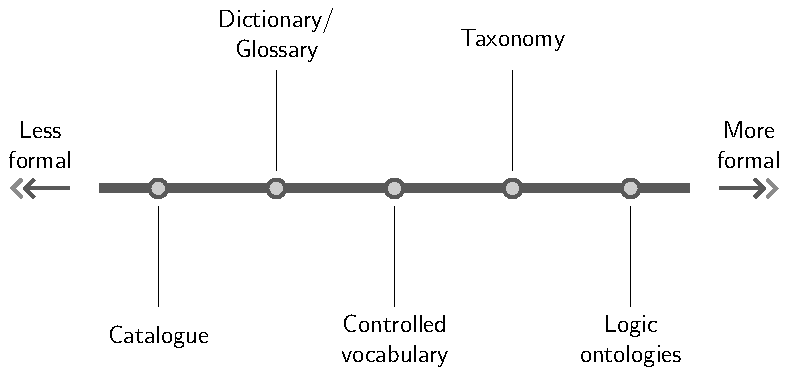
\includegraphics{images/spectrum.pdf}
    \caption[The spectrum of ontology formality]{This picture depicts the possible interpretations of what constitutes an ontology, arranged by formality levels. A \emph{catalogue} is a list of terms, with no definitions or relations between themselves; a \emph{dictionary} provides some textual definitions, as well as, possibly, synonyms; a \emph{controlled vocabulary} defines a standard set of terms to be used in a particular context, along with textual definitions, synonyms, related concepts, \etc.; a \emph{taxonomy} arranges the terms is a hierarchy, without formally defining what it means for a concept to be classified under another concept; and a \emph{logic ontology} provides machine-readable knowledge in a formal and precise way. Many other possible interpretations have been left out of this spectrum. Adapted from~\citep{McGuinness2002}.}
    \label{fig:spectrum}
\end{figure}

This spectrum can be used to distinguish some of the ontologies used by the biomedical informatics community. While the most recent ontologies, including most of the ontologies used in this work, have been developed using formal systems (\ie with the use of formal languages), some have still not been fully formalised. An example is the Medical Subject Headings (\ontology{MeSH}), which is a taxonomy of concepts that are related to one another by means of an underspecified relationship type. For example, \term{Head} is categorised under \term{Body Regions}, and \term{Ear} is categorised under \term{Head}, but while heads are body regions, ears are not heads; they are instead \emph{parts} of the head. This illustrates the informality of \ontology{MeSH}: only one relationship type exists, but it is used to express different notions.

% While most of the semantic similarity algorithms developed so far can be applied to semantic networks in general (to the best of my knowledge, using formal OWL constructions in semantic similarity algorithms has been first attempted in one of my papers~\citep{Ferreira2013}), this thesis will focus mainly on formal ontologies.

Contrast this with the far right end of the spectrum, occupied by fully formal ontologies. In these, complex logic-based assertions can be made about the domain being represented in the ontology. For example, one can express the notions that
\begin{paralist}
    \item \term{Square} and \term{Circle} are disjoint concepts (nothing can exist that is both a square and a circle);
    \item \term{Elephant} is a subclass of \term{Animal} (all elephants are animals); and
    \item a \term{Finger} is \prop{part-of} some \term{Hand}.
\end{paralist}

In order to develop fully formal ontologies, with formal-logic constructions that allow us to assert those types of facts (called \emph{axioms} in KR), several languages have been developed over the years, enabling knowledge engineers to formally represent the concepts of a domain and the relationships between those concepts. The current standard in KR is to use the Web Ontology Language (peculiarly, abbreviated as OWL). This language uses many first-order logic constructions to state facts about the concepts that are represented in the ontologies. OWL ontologies can be saved in files using different but equivalent formats, such as XML, Turtle or JSON. OWL semantics are specified by the World Wide Web Consortium, which defines how each construct should be interpreted and which logical conclusions can be deduced from them~\citep{Motik2012,Motik2012a}.

The most frequent construction in an ontology is the ``class-subclass'' relationship (variously called the \prop{is-a}, ``hypernymy'' or ``subsumption'' relation): \eg the concept \term{Elephant} is a ``hyponym'' of the concept \term{Animal}, since all elephants are animals (likewise, \term{Animal} is a ``hypernym'' of \term{Elephant}). Another common relationship between concepts is ``meronymy'', which is the relationship between the part and the whole, \eg a \term{Finger} is part of some \term{Hand}. A significant portion of the knowledge represented in an ontology can be visualised as a graph, where nodes are concepts and edges are relationships (\eg the class-subclass relationship, or the relationship between part and whole). The hypothetical ontology presented in \figref{fig:anatomy-ontology} shows this parallel between ontologies and graphs. Each of the edges corresponds to one of the axioms of the ontology and, therefore, to an asserted fact. Usually, the class-subclass hierarchy is represented as a tree, while the other relationships are represented as general edges between the nodes.

\begin{sidewaysfigure}
    \centering
    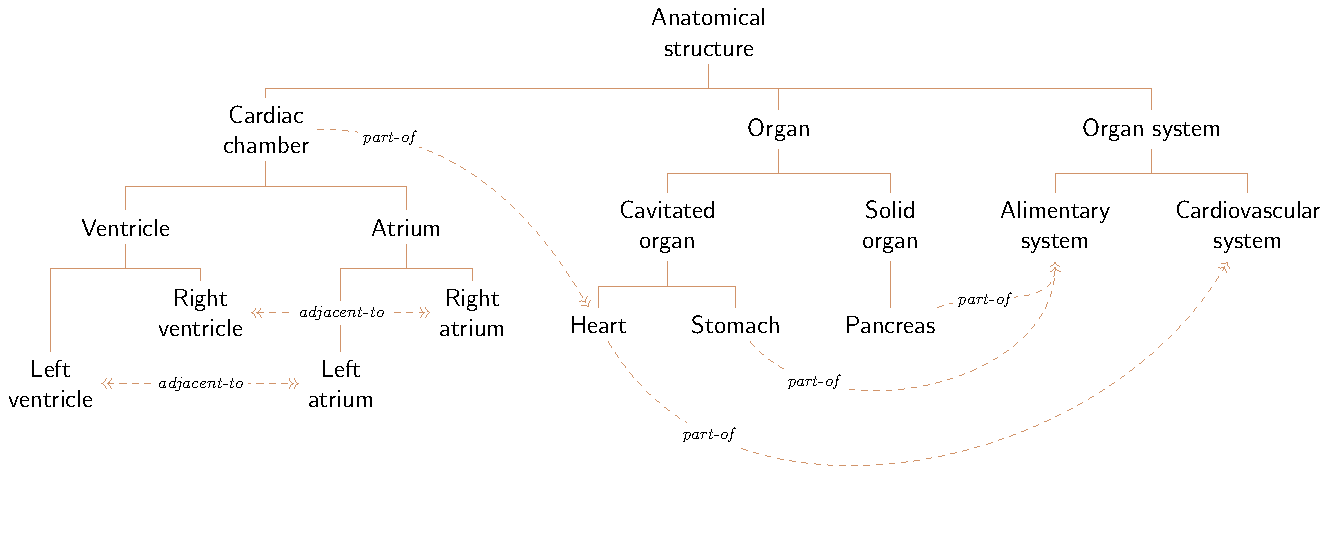
\includegraphics{images/anatomy.pdf}
    \vspace{-\baselineskip}
    \caption[A hypothetical ontology of human anatomical concepts]{This hypothetical ontology contains several concepts related to the domain of human anatomy. It includes concepts that are related to one another by means of the class-subclass relationship (in solid lines) and other types of relationship (in dotted lines, edges labelled with the type of relationship). A note for the reader: this image will be referenced throughout this chapter and the next \mdash take a moment to memorise that this is page number~\pageref{fig:anatomy-ontology}.}
    \label{fig:anatomy-ontology}
\end{sidewaysfigure}

In the biomedical domain, ontologies are often composed of concepts but not of actual instances of these concepts. For example, while the concept for \term{Head} exists in the human anatomy ontology, it being the machine-readable representation of all the human heads, the various instances of this concept (my head, the reader's head, and all human heads that ever existed and will ever exist) are not part of the ontology. In fact, since ontologies are abstractions over reality, they contain only facts that are true for all instances of a particular type. As such, they do not contain instances but instead represent concepts only.

As ontologies are inserted in a computer-science context, developing an ontology is in practice a two-sided task: on the one hand, it requires a logic background, since the formalisms of OWL are founded on first-order logic; on the other hand, it requires a background on the domain being represented in order for the ontology to be as accurate as possible. Beyond these inevitable prerequisites, building an ontology that aspires to be \emph{the} standard representation of a scientific field of research demands a significant commitment to the best practices of ontology development. For example, ontologies should be reusable, the concepts should have textual definitions for the benefit of its human users that are synchronised with the formal definitions (given by the axioms of the ontology that refer to the concepts), and the ontology should be kept updated in light of scientific advances, to guarantee its correctness~\citep{Noy2001}.

Additionally, ontologies should be as interoperable as possible. There is a project within the biomedical informatics community, the OBO Foundry, which specifies a set of principles that are designed to increase the interoperability of the ontologies, such as orthogonality between ontologies and reuse of concepts form one ontology to the next~\citep{Smith2007}. This ensures that each biomedical concept has a single representation and is, therefore, unambiguous.


\section{Web Ontology Language} \label{sec:concepts/owl}

While research on semantic similarity should be agnostic to the languages used to express the ontologies, in practice, the existence of standards and community-driven recommendations means that the majority of ontologies are expressed using the same standards. In fact, the Web Ontology Language~(OWL) is currently the language of choice to represent scientific knowledge, particularly in the biomedical domain. While other languages exist, largely due to historical reasons, they almost always have a translation to OWL.

For example, the OBO Foundry has been active since before OWL had been fully specified, and as such they have developed an ontology language of their own, called OBO (while the name is the same, OBO Foundry and OBO language are distinct concepts). With the standardization of OWL, however, OBO language has been almost completely deprecated: its constructions can be represented in OWL (\ie OBO is, semantically, a subset of OWL), and tools to convert from it to OWL have been developed.

Since my work was based on OWL ontologies, it is important to let the reader know some of the terminology and notation used by this descriptive language.

In general, OWL ontologies are a representation of the concepts that describe the domain of knowledge being encoded in the ontology. The basic object of an OWL ontology is therefore the \emph{class}: the representation of the real-world concept. Another important notion is the \emph{individual}, which is the representation of a real-world object relevant for the domain. For example, a human anatomy ontology would contain the class \term{Heart}, which can be thought of as the set of all the individual ``human hearts'': my heart, the reader's, and all other human hearts that have existed, exist in this moment, and will exist in the future.

OWL ontologies also make use of \emph{properties}, which are the ``verbs'' that represent the relationship between the individuals. For example, ``my heart'' \prop{has-part} ``my left ventricle''. Properties are exclusively asserted between individuals; however, the ontology can describe high-level collections of property assertions that are known to be true. For example, since all human hearts have one left ventricle, a human anatomy ontology contains an \emph{axiom} that represents this fact (see \figref{fig:anatomy-ontology}).

There are several types of axioms that can be asserted in an OWL ontology, which are the constructions of the ontology most closely based on the field of description logic and deductive reasoning. The types of axiom relevant for this work are the following:
\begin{itemize}
    \item The \emph{subclass of} axiom states that all the instances of one class are also instances of the other class: \eg ``$\term{Ventricle} \sqsubseteq \term{Cardiac chamber}$'' means that all ventricles are cardiac chambers.
    \item The \emph{disjointness} axiom between two states that there can never be an object that is simultaneously an instance of the two: \eg ``$\term{Ventricle} \,\sqcap\, \term{Atrium} \sqsubseteq \bot$'' means that there is no object in the real world that is both a ventricle and an atrium.
    \item The \emph{existential quantification} axiom states that instances of a class are related to an instance of another class by a certain property: \eg ``\existential{Heart}{has-part}{Left ventricle}'' means that every heart has a part that is a left ventricle.
\end{itemize}

The logical nature of these axioms are the main reason that ontologies such as \ontology{MeSH} are not on the same formality level than other carefully crafted logical ontologies. For example, a hypothetical axiom ``\existential{Head}{has-part}{Nose}'' (all heads have a nose), together with the fact that \term{Ear} is categorised under \term{Head} in this ontology, would lead to the incorrect inference that every ear has one nose.

While OWL allows the description of individuals, biomedical ontologies are developed and used as reference ontologies for various purposes and, as such, do not define any particular instance of their classes. They only describe the knowledge at the high level of the concepts.

Ontologies in general, and OWL ontologies in particular, make use of what is known as the \emph{open-world assumption}. Informally, this assumption states that what is not asserted does not give any information about what is known \emph{not} to be true. One consequence is that if an ontology does not contain subclasses for a given concept, it cannot be assumed that no such subclasses exist. A highly appropriate quote from Martin Rees~\citep{Oliver1971,Berendzen1973} perfectly encompasses this assumption:
\begin{quote}
    Absence of evidence is not evidence of absence.
\end{quote}
This has significant impact on the rules of inference that are allowed in OWL ontologies, and has consequences to the overall research performed in this area, as we will see later in \chpref{chap:enhancements}.

Being part of an effort to make knowledge more accessible to machines, OWL language uses the idea of \emph{universal identifiers}. The Internationalized Resource Identifier (IRI) are, superficially, similar to URLs. For example, the most abstract concept that can be used in an OWL ontology is \nolinkurl{http://www.w3.org/2002/07/owl\#Thing}, a class that contains all instances. This identifier can be used in any OWL ontology with the meaning defined by the World Wide Web Consortium (W3C). Likewise, any identifier that is a valid IRI can be used by any OWL ontology, and the universal nature of the identifier assures both developer of the ontology and its users that the class represents the concept defined in the ontology where it was originally created.


\section{Semantic web} \label{sec:concepts/semantic-web}

Once knowledge has been made machine-readable by using ontology concepts and entity annotation, it needs to be stored and shared amongst interested parties. This idea of publishing and sharing machine-readable information has been made possible by the semantic web, which prescribes both
\begin{paralist}
    \item a set of standard formats for representing knowledge (of which OWL and IRI are examples); and
    \item a collection of technologies to deal with knowledge (such as reasoning over OWL ontologies).
\end{paralist}
In particular, the semantic web is a vision of information management and sharing that promotes intelligent access to data on the World Wide Web, both by humans and by computers~\citep{Berners-Lee2001,Shadbolt2006}. It is especially useful for handling heterogeneous data, since it was designed with a structured yet flexible operation mode.

The semantic web is build around the idea of expressing information in structured and formal languages, such as the Resource Description Framework (RDF), that allow the expression of precise statements (\eg ``Mary'' \prop{has-father} ``Peter''). At the most basic layer, the semantic web does not define what the property \prop{has-father} means, working instead as a framework for sharing formal statements, which allows users with the necessary knowledge to deal with this information according to their needs. At a higher layer, semantic web \emph{does} use the expressive and logical power of ontologies, enabling data to be effectively searched based on its semantics rather than its syntax. For example, with an ontology that contains the fact that the property \prop{has-father} is the inverse of \prop{father-of}, a user can search in a data repository for the objects~$x$ that satisfy the expression ``Peter'' \prop{father-of}~$x$, and still find the answer ``Mary'' (along with all her siblings, if any exist in the repository): while this exact statement was never introduced in the repository, the inverse statement was, and the relation between the properties \prop{has-father} and \prop{father-of} allows the search engine to correctly \emph{infer} this answer. This illustrates one of the most important characteristics enabled by the semantic web: interoperability of data. On the one hand, information is shared using standard formats; on the other hand, the semantics associated with the information, \ie the meaning and the implications of the data, are formalised based on the precise semantics of the languages used to describe it. This enables data owners to describe their data using as much precision as deemed necessary, while allowing researchers to query the data being as general as they want, while still guaranteeing that the relevant information is retrieved.
\looseness=1

The use of reasoners enables the production of new data, and allows computers to process the structured information based on their actual semantics. An example of semantic web in action can be seen in the work by~\citet{Lopes2012}. These authors have developed a framework capable of integrating structured knowledge from various sources in a single platform, which is enriched with web services that enable \emph{knowledge federation}, \ie the possibility to query data wherever it resides, without the need to add it to a local repository. The formality behind semantic web data suggests that these data can be linked with other information~\citep{Bizer2009, Bizer2009a}, just like documents in the web are linked to each other.

An interesting example of the semantic web in action is the use of linked data to cross information on some epidemiological surges with the characteristics of the locations where these surges started (\eg the socio-economic or environmental conditions). To illustrate, consider a collection of epidemiological surges together with a repository containing characteristics of geographical locations. The search presented in \lstref{lst:sparql} is written in SPARQL, a language that expresses queries over RDF stores (also a standard proposed and promoted under the semantic web movement~\citep{Harris2013}). If presented to the correct data repositories, it would return the characteristics of the places where the ``H1N1 surge of 2009'' started. Then, comparing the returned information with the results for other epidemic surges, it would be possible to detect the characteristics more strongly associated with each one, and to find patterns in the data.

\begin{listing}[t]
\centering
\begin{minted}[gobble=4]{sparql}
    PREFIX epidemic: <http://www.epidemiology.com/data/>
    PREFIX geo: <http://www.geography.com/data/>
    
    SELECT ?characteristic
    WHERE {
        epidemic:H1N1_surge_of_2009 epidemic:surge_started_in ?location .
        ?location geo:has_characteristic ?characteristic .
    }
\end{minted}
\caption[Finding the characteristics of the starting place of an epidemic with SPARQL]{This query retrieves the information we are looking for. Notice that it depends on non-existing repositories (\nolinkurl{http://www.epidemiology.com/data} and \nolinkurl{http://www.geography.com/data}) and, as such, is not functional. Even if these repositories existed, the query would only work if \mintinline{sparql}{geo:has_characteristic} was a superproperty of all the relevant properties.}
\label{lst:sparql}
\end{listing}

Another relevant example of semantic web in action is the Open PHACTS project~\citep{Williams2012}, which provides an integrated and interoperable platform that aims at reducing barriers in pharmacology, specially in the task of drug discovery. The general methodology followed for this endeavour is the adoption of semantic web technologies, such as RDF stores, semantic annotation (see next section), SPARQL queries, \etc.\ which are integrated in the platform, thus building on open standards to ensure wide applicability of the approaches used for integration of data.


\section{Semantic annotation} \label{sec:concepts/semantic-annotation}

Ontologies, standing on their own, define a set of unambiguous, objective and traceable concepts, along with their names, synonyms, and (formal or textual) definitions. However, as knowledge artefacts, ontologies do not \emph{do} anything. Using an analogy, ontologies are to knowledge as the source code of a program is to the program itself. They are specifications packed with a lot of potential, and liberating this potential is possible only with the right set of tools, giving researchers the ability to explore the knowledge they contain. Therefore, it is essential for the advancement of science that the community develops and uses ontologies in a way that can be stacked with current technologies designed for this area. In fact, the knowledge that is stored in an ontology can be quite expressive, depending on its format and how formal its representation is, and can be explored in various ways.

For example, repositories enriched with ontology axioms can be paired with SPARQL to allow intelligent search of data within the repository (see \lstref{lst:sparql}). We will see in \secref{sec:concepts/semantic-similarity} that another such technology is semantic similarity (the primary subject of this document), which calculates similarity between entities based on the knowledge that is associated with them.

Right before discussing semantic similarity, however, it is important to understand \emph{what} is usually compared with this technique. Comparing concepts with concepts is not always useful, and ideally we would like to compare full entities (clinical notes, proteins, disease, \etc.)\ which are usually \emph{annotated} with ontology concepts but are not themselves concepts. For example, a common practice in biology is annotating proteins with their functions. It is almost universally accepted that protein functions are well represented in the Gene Ontology (\ontology{GO}). With this ontology, the information that a gene is responsible for a specific function can be expressed, \eg the protein ``telomerase'' \term{UniProt:Q99973} is annotated in the UniProt database as having the function ``ATP binding'' \term{GO:0005524} and being localised in the ``nuclear matrix'' \term{GO:0016363}). This statement is objective, unambiguous (\ie it does not depend on the researcher that made the statement, nor on any other context), universal, and traceable. Databases like AmiGO~\citep{Carbon2009} are dedicated to managing statements like this.

These annotations can be seen as a semantic description of the protein, since they can be used to, computationally, ascribe to the protein a meaning more complex and informative than simply its sequence. There are automatic tools that reason over \ontology{GO} annotation in order to help interpret the results of experimental procedures. For example, Gene-Set Enrichment Analysis determines, based on the gene expression levels in a wild-type individual \vs those of a mutated individual, which \ontology{GO} molecular functions are most strongly associated with the mutated individuals~\citep{Subramanian2005}. This can help identify, for instance, molecular causes of a disease. Relying on ontology concepts to annotate biomedical entities allows automatic reasoning to be applied directly to them, increasing the amount of automation that can in theory be applied in biomedical research.

In many cases, the annotations of an entity span more than one ontology. In epidemiology, a single dataset may require annotation with diseases, geographical locations, medical procedures, socio-economic conditions, \etc.; kinetic models of chemical reactions use concepts representing chemical compounds and the mathematical equations for the reaction's velocity. Given this multidisciplinarity, it is essential that the standard ontologies used throughout the community can work together, providing users with the confidence that their annotations are interoperable. As discussed previously, this is the case with most ontologies of the biomedical domain. For example, some proteins capture ethanol molecules, a function represented in \ontology{GO} with the concept \term{Ethanol binding}. This concept is related to \term{Ethanol}, itself represented in \ontology{CHEBI}. Such interoperability also has the advantage of minimising the risks of representation duplication (akin to ``code duplication'' in software development).

Finally, semantic annotation is itself a form of knowledge representation. By stating, in a machine-readable format, that some protein performs a certain function in the cell, we are augmenting the amount of knowledge that can be exploited by computational methods.


\section{Semantic similarity} \label{sec:concepts/semantic-similarity}

Now that some preliminary concepts have been introduced, we are finally ready to appreciate the notion of semantic similarity.

Traditionally, computers have been able to compare objects that can be represented either mathematically (\eg vectors) or as strings of characters (\eg gene sequences). However, the algorithms that are used with these structures are context-free: they usually transform the structures without any knowledge of what they represent. With the help of a formal representation of knowledge, computers are given the ability to manipulate concepts that are difficult to represent in a mathematical way.

Knowledge representation (by means of ontologies and semantic annotation) provides the appropriate support for automatic manipulation of information. In this context, semantic similarity is a technique that assigns a numeric value to a pair of concepts or annotated entities based on the similarity of their \emph{meaning}, which is automatically extracted from the ontologies.

For example, there is no directly obvious way to compare two anatomical entities. However, considering the illustration in \figref{fig:anatomy-ontology} (page~\pageref{fig:anatomy-ontology}), it is possible to intuitively understand that, because both a \term{Heart} and a \term{Stomach} are examples of a \term{Cavitated organ}, they are more similar than \term{Heart} and \term{Pancreas}. This intuition can be captured in a formal algorithm: \term{Heart} and \term{Stomach} are both subclasses of the concept \term{Cavitated organ}, while \term{Heart} and \term{Pancreas} are subclasses of the concept \term{Organ}, a less specific concept. The fact that this measure of similarity makes use of the meaning of the concepts, as represented in the ontologies, has impelled the use of the phrase ``semantic similarity'', first used in this context by~\citet{Resnik1995}. Although the meaning of a concept is also non-mathematical, it is possible to use ontologies as proxy for that meaning and KR technologies to manipulate it. For this reason, semantic similarity can also be called ``ontology-based similarity''. For the purpose of this thesis, I define semantic similarity as follows:

\begin{quote}
    A semantic similarity measure is an algorithm that takes as input a pair of ontology concepts (\emph{resp.}~a pair of entities annotated with ontology concepts), and returns a numeric value that reflects how similar the concepts (\emph{resp.}~entities) are; the meaning of the concepts being compared (\emph{resp.} used to annotate the entities) is retrieved from the ontologies where they are defined.
\end{quote}

Semantic similarity has been applied in several areas of research. \citet{Hoehndorf2013} provide a collection of applications that contribute to verifiable scientific advances. Some examples collected by me during my research are:
\begin{itemize}
    \item predicting protein interactions (either physical interaction, as part of the same complex, or less obvious interactions, like being part of the same metabolic pathway)~\citep{Azuaje2004,Guo2006,Wu2006};
    \item predicting sub-cellular location of proteins~\citep{Lei2006};
    \item predicting whether a disease affects a certain body part~\citep{Ferreira2011};
    \item finding protein complexes in protein-protein interaction networks~\citep{Li2010b};
    \item helping the differential diagnosis process by suggesting diseases based on a set of symptoms~\citep{Kohler2009};
    \item predicting chemical properties in small metabolites~\citep{Ferreira2010};
    \item finding new putative uses for drugs that are currently being used (drug repositioning)~\citep{Tan2014};
    \item assisting visualization techniques by finding representative concepts in a large set~\citep{Supek2011};
    \item being part of large information retrieval systems~\citep{Emadzadeh2014};
    \item determining the meaning of ambiguous terms~\citep{McInnes2011,Hu2012,Goeg2014};
    \item improving the classification of clinical texts based on machine-learning~\citep{Garla2012a}; and
    \item assisting text-mining by providing a means to detect similarities in meaning that are not obvious using string-similarity measures~\citep{Spasic2005,Varelas2005} and by disregarding some mined facts if they fail to verify a constraint on semantic similarity~\citep{Lamurias2015}.
\end{itemize}

% In practice, semantic similarity has been primarily calculated for concepts from the same ontology or entities annotated with concepts from the same ontology, never mixing more than one ontology. In \secref{sec:sota/multi}, I will make some references to past literature that uses multiple ontologies, but the truth is that this is a topic that has not yet been properly tackled. In fact, while multiple ontologies have been used to compute semantic similarity, this has never been explored in a \emph{multi-domain} context.

The notion of similarity it tightly coupled with the notion of \emph{relatedness}. From a technical point of view, similarity and relatedness are the same idea: they assign a value to a pair of concepts\slash pair of annotated entities. As such, distinguishing between the two ideas is generally difficult. As a rule of thumb, it has been proposed that similarity is context-independent (it takes into account the concepts being analysed but disregards the application under which they are being compared) and relatedness depends on the goals behind the analysis~\citep{Budanitsky1999}. \citet{Pedersen2007} were amongst the first to make a more formal distinction between these two ideas: similarity is a special case of relatedness that considers only the hypernymy of concepts (the class-subclass hierarchy), while relatedness explores all other kinds of properties in the ontologies.

Take, for instance, the concepts \term{Heart} and \term{Blood}. In the biomedical field, they are closely related, since the function of the former is to pump the latter. In gastronomy, there is little relatedness between the two. Independently of the context, however, a heart is not at all similar to blood: one is an organ, the other a biological fluid (in fact, a liquid tissue).

\begin{figure}
    \centering
    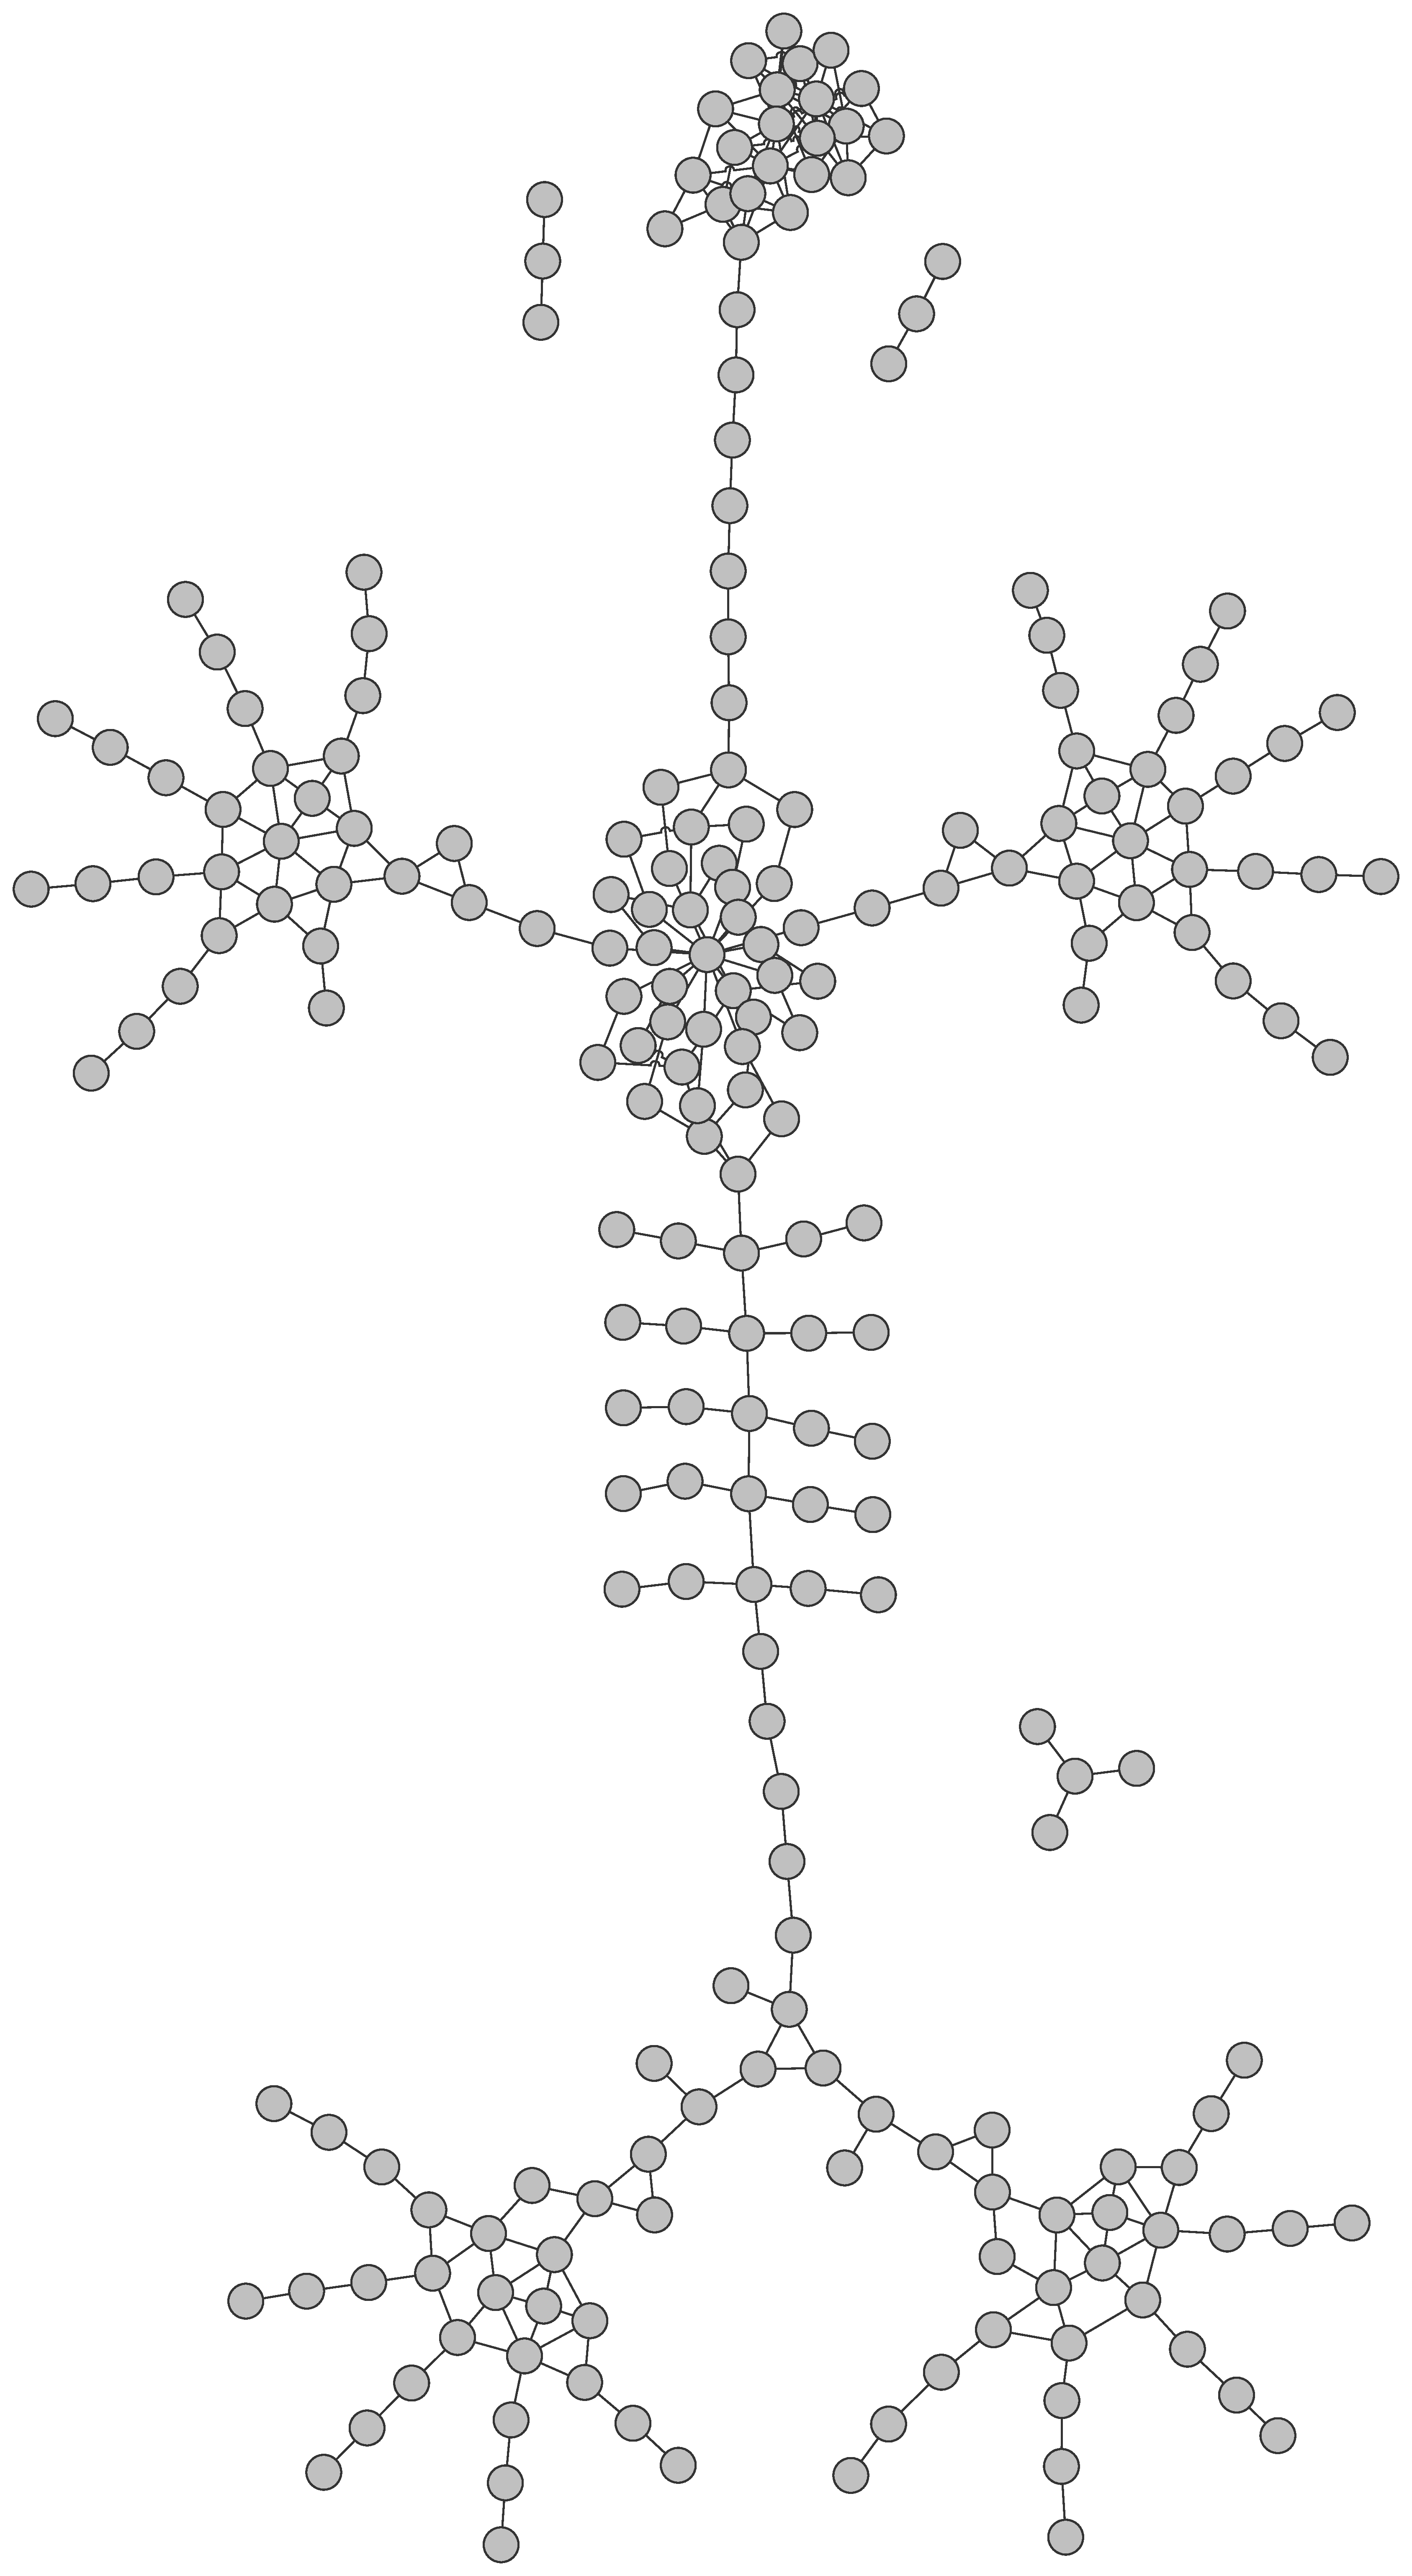
\includegraphics[height=0.7\textheight]{images/skeleton.pdf}
    \caption[Graph describing the \prop{articulates-with} property in \ontology{FMA}]{Each node is a concept from \ontology{FMA} representing a human bone, and each edge represents the fact that the two concepts are related to one another by means of the \prop{articulates-with} property. Features of the human body visible in this picture include: the head, the rib cage, the two hands and their fingers, the ``false ribs'' (which do not articulate with the sternum), the vertebrae, the two feet and their toes, and also the two sets of ear bones, which are disconnected from the rest of the body.}
    \label{fig:skeleton}
\end{figure}

In fact, in some contexts, the use of properties other than the class-subclass relationship can be useful to find patterns in data or to infer new conclusions. Consider the graph drawn in \figref{fig:skeleton}. This figure was obtained by drawing an edge between two anatomical concepts from \ontology{FMA} (the Foundational Model of Anatomy) if the two are related by means of the property \prop{articulates-with}: hence, each node is a bone and the edges show that there is an articulation between the two bones. A graph editor was then used to automatically layout the nodes (I used yEd). Finally, minor manual adjustments were carried out, both to rotate the image and to move the three disconnected subgraphs. Upon closer inspection, it is evident that the graph mirrors a slightly deformed human body, with a head, two hands, a spine, and two feet: the head is tangled because most bones articulate with a large set of other bones, and the rib cage is also tangled because the upper ribs connect both to the spine and the sternum (the two disconnected pieces on the top are the bones of the ear; the third disconnected piece is a bug in the ontology). That this picture is obtained with minimal human intervention and that, even so, it so closely resembles the human body, which is the object being represented in \ontology{FMA}, is extremely provoking evidence that relationships other than hypernymy are vital to properly process scientific knowledge.

In the context of multi-domain similarity, relatedness has, in fact, high utility. Consider now the concepts \term{Otitis} and \term{Ear}, likely to be represented in different ontologies: one for diseases and the other for anatomical entities. Despite being from different ontologies, there is a strong relation between the two, as otitis is an infection of the ear. In the context of diseases, this relationship increases the relatedness between \term{Otitis} and other ear diseases (\eg \term{Hereditary deafness}), which is difficult to capture using similarity alone, since an \term{Otitis} is an inflammatory disease and \term{Hereditary deafness} is a genetic disease. In such a disease hierarchy, it is impossible to obtain an accurate comparison value between the two diseases based on the class-subclass hierarchy only. In fact, we know that \term{Otitis} is an ``\term{Inflammatory disease} that \prop{is-located-in} some \term{Ear}'' and that \term{Hereditary deafness} is a ``\term{Genetic disease} that \prop{manifests-in} some \term{Ear}''. Therefore, exploring the relationships between the concepts other than the class-subclass hierarchy can help increase the accuracy of semantic similarity.

% Incidentally, there are often practical reasons to discourage what is known as the multiple-inheritance pattern in ontology development, \ie the practice of assigning more than one direct superclass to any concept (advantages include an easier development, since errors are easier to debug in this pattern)~\citep{Aranguren2010}. Under this restrain, \term{Otitis} cannot be formally defined as simultaneously an \term{Inflammatory disease} and and \term{Ear disease}.

The concept of distance measures should also be mentioned. Before ontologies were used to compute similarity measures, they were used to compute distances between concepts~\citep{Rada1989}: for a pair of concepts that are close in meaning, similarity values are high and distance values are low. Although there is no unique way to convert a distance into similarity, some formulae have been frequently used. Denoting distance with~$d$ and similarity with~$\sigma$, they are
\begin{itemize}[itemsep=0pt]
    \item $\sigma = 1/d$;
    \item $\sigma = D - d$ where $D$~is the maximum possible distance, and
    \item $\sigma = e^{-\gamma \cdot d}$ for some~$\gamma > 0$.
\end{itemize}
% Distance measures are usually constructed as metrics, satisfying the following three conditions:
% \begin{itemize}[itemsep=0pt]
%     \item identity of indiscernibles:~$\forall x \; d(x, x) = 0$;
%     \item symmetry:~$\forall x,y \; d(x, y) = d(y, x)$; and
%     \item the triangle inequality:~$\forall x,y,z \; d(x, z) \leq d(x, y) + d(y, z)$.
% \end{itemize}
% It has been argued, however, that both symmetry and the triangle inequality can produce unintuitive results when measuring semantic distance between concepts~\citep{Tversky1977,Bowdle1997,Janowicz2007}.




% \section{Information Content} \label{sec:concepts/information-content}

% For a period of time, the notion of an ontology-based semantic similarity measure exploited mainly the distance between two concepts measured in the number of edges between them (see, for an example, the illustration in \figref{fig:distance} for a brief visual summary of that idea). \citet{Resnik1995} introduced the idea of \emph{information content} (IC) to measure how much information is carried out by each concept.

% For example, \term{Animal} can refer to many distinct concepts, and, as such, carries a small amount of information when compared to the concept \term{Dog}, which has a more informative definition. Another way to understand the idea of IC is as a measure of specificity: \term{Dog} is more specific than \term{Animal}. It has been shown that measures that use the notion of IC to weight the concepts of an ontology perform better than those that rely on edges alone~\citep{citation required}. The main reasons for this to happen are that (i) nodes and edges are seldom uniformly distributed throughout the various levels of the class-subclass hierarchy, (ii) edges at the same level do not necessarily correspond to the same semantic distance between concepts and (iii) nodes at the same level do not necessarily have the same specificity~\citep{Pesquita2009}. A simple example shows these faults: the intuitive distance covered by the relationship ``\term{Fungal spore} \prop{is-a} \term{Spore}'' seems to be narrower than the distance in ``\term{Plankton} \prop{is-a} \term{Organism form}'' (examples taken from \ontology{MeSH}).\margin{Maybe use another example from one of the ontologies that will be used in the thesis?}


\section{Multiple-ontology context} \label{sec:concepts/multi-ontology}

As with other emergent fields, the practice of ontology development has been tackled by various people, from hobbyists to philosophers, from scientific research teams that need the power of ontologies for their research, to enterprises that sell their knowledge representation of reality. This can lead to many different ontologies being constructed by different people, with either a different philosophical base or simply a different perspective of reality.

The dissemination of ontology construction and usage places the utility of ontologies in a vantage point, mainly due to two facts:
\begin{paralist}
    \item different interpretations of reality can lead to complementary ontologies, and
    \item a variety of domains of knowledge are getting represented as ontologies, especially by those more competent to do so, \ie people with a background knowledge in these domain.
\end{paralist}

With such a plethora of ontologies available, it is not surprising to notice that many applications are now making use of more than a single ontology. For example, the Epidemic Marketplace~\citep{Lopes2010} uses a number of epidemiology-related ontologies to annotate its resources~\citep{Ferreira2012}, thus connecting a web resource to various concepts from different domains. Another example are models of biological systems, also being annotated with multiple ontologies: with the processes they model, the chemical molecules and cellular components involved in those processes, the physical quantities that they model, \etc.~\citep{Li2010a,Juty2015}. To properly achieve a significant semantic similarity measure between such multidisciplinary entities, it is essential that a multi-domain measure be developed.

\begin{figure}
    \centering
    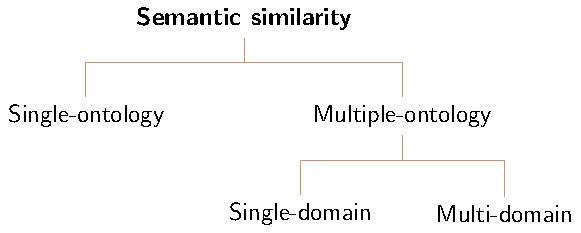
\includegraphics{images/multi-domain-similarity-categories.pdf}
    \caption[Categories of semantic similarity]{Semantic similarity (and relatedness) can be made in a single- or multiple-\emph{ontology} context; but using more than one ontology does not immediately imply a multi-\emph{domain} context, since some ontologies can model the same domains of reality (for example \ontology{MeSH} and \ontology{NCIt} overlap in some of their concepts). As such, multiple-ontology analysis can be further subdivided into single- and multi-domain.}
    \label{fig:multi-domain-similarity}
\end{figure}

Consider the categorization of semantic similarity methods illustrated in \figref{fig:multi-domain-similarity}. Both concepts \term{Heart} and \term{Blood} can be included in an ontology of anatomy and, therefore, their similarity can be computed with a single ontology. However, biomedical ontologies are often incomplete, due to the intrinsic uncertainty associated with the scientific field; they can also contain errors, or can even follow a certain view of reality that is not shared amongst everyone. In each of these cases, a second ontology may be used to offer a complementary view of reality so that incompleteness, errors and subjective interpretations are mitigated. ``Multiple-ontology single-domain'' similarity can be used to handle this situation \citep[\eg][]{Al-Mubaid2009}. In this approach, two or more ontologies representing the same domain are used in a complementary way to improve semantic similarity results.

Multiple-domain similarity represents a step beyond this approach, since it uses multiple ontologies from distinct domains in order to compare concepts in a multidisciplinary context. This is necessary, for example, when performing relatedness analysis, such as when comparing diseases with symptoms, or symptoms with anatomical entities, but also when comparing entities that are annotated with concepts from other domains. For example, the concepts \term{Heart} and \term{Blood}, previously used in the example of single-ontology similarity, can be compared based on their functions, the symptoms they exhibit, or even, if appropriate, their use in gastronomy.


\section{Summary} \label{sec:concepts/summary}

In this chapter, I exposed some of the most important concepts necessary to understand the rest of this document. I started by visiting the notions of knowledge representation and ontologies as computational artefacts, thus laying down a theoretical framework that enables the representation of unstructured information in a way that can be parsed and acted upon by machines. I then mentioned the ideas of semantic web and semantic annotation, which are the response of the scientific community to that theoretical framework: they define the standards that are used to store and share information among the ones representing the knowledge and the ones using that knowledge. At last, I described semantic similarity as one of the techniques that uses information from ontologies, with several possible objectives, and the fact that multi-domain semantic similarity seems to be useful and, yet, underdeveloped.

The next chapter will describe some of the methodologies that have been proposed to calculate semantic similarity, including both historical and state-of-the-art measures.

\chapter{State of the art} \label{chap:sota}

This section is an exposition of both an historical and current state-of-the-art in semantic similarity calculation. It starts by describing the first few measures and how they evolved through time. Throughout the chapter, I present both the concepts behind the measures of similarity proposed by various researchers and some selected formulas used by these measures.


\section{The art of semantic similarity} \label{sec:sota/art}

The study of semantic similarity has been subject of research for a significant amount of time. A first work by \citet{Tversky1977}, published in \emph{Psychological Review} laid the first steps in the formalism of the mathematical calculation of similarity by developing a theory that tries to explain similarity as judged by people. In this work, similarity is described as a function of the features of the things being compared, namely common features \vs distinctive features, \eg shape for geometric figures or political aspects for countries.

A previous idea was published some years before by \citet{Quillian1968} and \citet{Collins1975} (these have no notion of similarity being calculated by computers, but instead lay down some theoretical psychological views on how people perceive similarity), which proposes that the mental processes by which humans organise their memories and concepts are based on a network of connected concepts, whose connections are stronger for more related concepts.

With the advent of computerised science, the idea that automatic systems could be able to compare concepts and other knowledge artefacts started to emerge, and thus the idea of semantic similarity was introduced.


\section{Edge-based approaches} \label{sec:sota/edge}

The works mentioned in the previous section have prompted \citet{Rada1989} to create a first measure of semantic distance based on a hierarchy of concepts, in this case the Medical Subject Headings (\ontology{MeSH}). They calculated distance as a function of the number of class-subclass relationships that must be traversed in order to go from one concept to the other in the hierarchy (also called the ``edge distance''). For example, using the ontology snippet in \figref{fig:anatomy-detail}, the edge distance between \term{Left ventricle} and \term{Right ventricle} is~$2$, and the edge distance between \term{Left ventricle} and \term{Right atrium} is~$4$. This vision of semantic analysis draws from the idea that an ontology can be represented as a tree, explained previously in \secref{sec:concepts/ontologies}. In fact, the use of trees to represent ontologies has become so widespread in this area that it is customary to use the notions of ``ancestors'' (\emph{resp.}~``descendants'') of a concept as the set of its direct and indirect hypernyms (\emph{resp.}~hyponyms), thus making \term{Ventricle} an ancestor of \term{Left ventricle} and a descendant of \term{Cardiac chamber}.

\begin{figure}
    \centering
    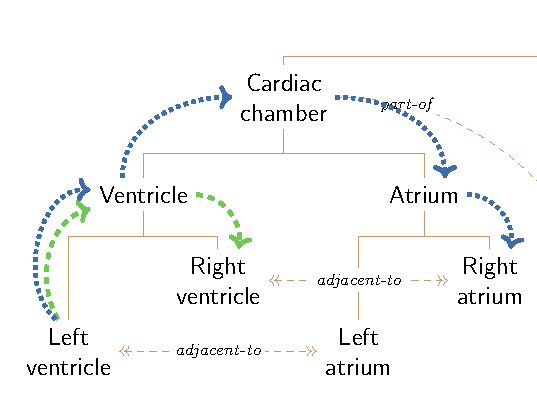
\includegraphics{images/anatomy-detail.pdf}
    \caption[Semantic measures explained in a hypothetical hierarchy]{This small detail of the hypothetical ontology presented in \figref{fig:anatomy-ontology} (page~\pageref{fig:anatomy-ontology}) includes further information representing one of the core ideas behind semantic measures. The concepts \term{Left ventricle} and \term{Right ventricle} are direct subclasses of \term{Ventricle}. As such, the edge distance between the two concepts is~$2$, as one has to climb up through the $\term{Left ventricle} \rightarrow \term{Ventricle}$ relationship and then down through the $\term{Ventricle} \rightarrow \term{Right ventricle}$ relationship to go from one concept to the other (see the green dashed arrows). Similarly, the edge distance between \term{Left ventricle} and \term{Right atrium} is~$4$ (blue dotted arrows).}
    \label{fig:anatomy-detail}
\end{figure}

Edge distance can be converted into similarity as detailed in \secref{sec:concepts/semantic-similarity}. For example, the work by \citet{Pedersen2007} refers to the use of $\sim(a,b) = 1 / p(a,b)$, where $p(a,b)$~is the number of nodes in the shortest path between concepts $a$ and~$b$. \citet{Wu1994} propose a normalization, using for that effect the notions of the \emph{least common subsumer} (LCS) between $a$ and~$b$, which is the most specific concept that subsumes both $a$ and~$b$ (\eg the LCS between \term{Left ventricle} and \term{Left atrium} is \term{Cardiac chamber}) and \emph{depth} of a concept, which is the edge distance between the root of the ontology and that concept:
\begin{equation}
    \sim[Wu](a,b) = \frac{2\delta(a,b)}{p(a,b) - 1 + 2\delta(a,b)}
    \label{eq:wu}
\end{equation}
where $\delta(a,b)$~is the depth of the LCS between $a$ and~$b$.

While intuitive, these approaches assume some things that are not always true in the biomedical domain:
\begin{paralist}
    \item the amount of concepts and class-subclass relationships is uniform throughout the various sub-domains represented in the ontology; and
    \item class-subclass relationships at the same depth in the ontology correspond to the same semantic distance between the two concepts.
\end{paralist}
In fact, concepts are denser where they represent more ``appealing'' areas of research, as that is where research focusses and, as such, where the community's knowledge is more detailed. A simple example shows these faults: the intuitive distance covered in ``\term{Fungal spore} \prop{is-a} \term{Spore}'' seems to be narrower than the distance in ``\term{Plankton} \prop{is-a} \term{Organism form}'' (examples taken from \ontology{MeSH}). Strategies have been proposed to attenuate these issues, such as weighting edges differently according to their hierarchical depth, or to node density and type of link~\citep{Pesquita2009}.


\section{Node-based approaches} \label{sec:sota/node}

Because of the problems mentioned above, focus changed from the edges to the nodes of the graph representation of the ontology. \citet{Resnik1995} proposed an information-theoretic notion called Information Content (IC), which depends on the frequency with which this concept is used to annotate entities in a corpus. For example, \term{Organ} can refer to many distinct concepts, and, as such, carries a small amount of information when compared to the concept \term{Heart}, which has a more informative definition; this measure, thus, reflects the \emph{specificity} of a concept. \citet{Resnik1995} has shown that measures that use the notion of IC to weight the concepts of an ontology perform better than those that rely on edges alone. (Note, however, that IC-based measures are also biased, as the annotation process is guided by the trends in research and, as such, there are more annotations made to concepts more related to ``hot'' research topics.)

The idea of using IC in semantic similarity is that it allows the definition of \emph{shared information} between concepts. Reusing the example from \figref{fig:anatomy-detail}, \term{Left ventricle} and \term{Right ventricle} share between themselves the definition of \term{Ventricle} (\ie \term{Ventricle} is a common superclass of both). Since IC reflects specificity, the similarity between two concepts can be computed as the IC of their most informative common superclass. This results in the intuitive notion that \term{Left ventricle} is more similar to \term{Right ventricle} (both are \term{Ventricle}s) than to \term{Right atrium} (they share only the fact that they are both \term{Cardiac chambers}), since \term{Ventricle} is more specific than \term{Cardiac chamber}.

The original work by \citet{Resnik1995, Resnik1999} defined the information content of a concept~$c$ based on ideas from information theory:
\begin{equation}
    \IC[Resnik](c) = -\log f(c)
    \label{eq:resnik-ic}
\end{equation}
where~$f(c)$ is the frequency with which concept~$c$ appears in a selected corpus. For example, in WordNet, a taxonomy of English words~\citep{Miller1995}, the number of occurrences of a concept is counted as its frequency in a collection of texts; for \ontology{GO}, \citet{Lord2003} measured the frequency of a concept as the number of proteins in the SwissProt database that are annotated with that concept. It is important to notice that a reference to a particular concept, \eg \term{Left ventricle}, is also a reference to its hypernyms, in this case \term{Ventricle}, \term{Cardiac chamber} and~\term{Anatomical structure}~(\cf \figref{fig:anatomy-ontology} on page~\pageref{fig:anatomy-ontology}). With this rule, it becomes trivial to prove that as one moves from abstract to specific concepts, the IC increases, as is expected for any measure of specificity.

The notion of information content, however, need not necessarily require the exploration of external corpora. It is possible to measure the specificity of a concept based on the structure of the ontology itself: for example, the number of concepts that are subsumed by~$c$ is intuitively higher for less specific concepts, while the concepts with no subclasses (sometimes called the \emph{leaves} of the ontology) are the most specific concepts. \citet{Seco2004} use this idea in order to define an \emph{intrinsic} measure of information content:
\begin{equation}
    \IC[Seco](c) = 1 - \frac{\log N_d(c)}{\log N}
    \label{eq:seco}
\end{equation}
where $N_d(c)$~is the number of direct and indirect hyponyms of concept~$c$ (including~$c$ itself) and $N$~is the total number of concepts in the ontology. As previously, more abstract concepts will have a lower IC value. This measure is adapted from \eqref{eq:resnik-ic} by taking $f(c)=\frac{N_d(c)}{N}$ and normalising so that the highest possible~$\IC$ is~$1$.

The main advantage of intrinsic IC measures is that they are independent of external resources, and, therefore, can be calculated using the ontology alone. A review by \citet{Sanchez2011e} shows that intrinsic methods do, in fact, correlate better with human judgement of similarity. This evaluation, however, is done on a set of $30$~pairs of concepts from WordNet. This is a very small number of pairs to use in an evaluation, given the size of WordNet; additionally, given its domain, WordNet is, in some senses, different to the ontologies used in biomedical research, as concepts in WordNet have a collection of meanings (many English words have, in fact, more than one definition), while the concepts from biomedical ontologies strive to be unambiguous. As such, these results may not be true for the biomedical domain.

Using such measures of specificity, it is possible to estimate the similarity between two concepts as the IC of their most informative common ancestor:
\begin{equation}
    \sim[Resnik](a,b) = \max_{c\,\in\,\CA(a,b)} \IC(c)
    \label{eq:resnik-ssm}
\end{equation}
where $\CA(a,b)$~is the set of all hypernyms common to both $a$ and~$b$. This was in fact the first node-based measure ever proposed~\citep{Resnik1995}. For example, in the ontology in \figref{fig:anatomy-ontology} (page~\pageref{fig:anatomy-ontology}), $\CA(\term{Heart}, \term{Stomach}) = \{\term{Cavitated organ}, \term{Organ}, \term{Anatomical structure}\}$ and since \term{Cavitated organ} has the highest IC in this set (it is the most specific), $\sim(\term{Heart},\term{Stomach}) = \IC(\term{Cavitated organ})$. The notion of \emph{most informative common ancestor} (MICA) is so widespread that it has its own mathematical definition:
\begin{equation}
    \MICA(a,b) = \argmax_{c \, \in \, \CA(a,b)} \IC(c).
    \label{eq:mica}
\end{equation}
Likewise, the idea of measuring the shared information content between two concepts as the IC of their MICA is also so common that I use a notation for that as well:
\begin{equation}
    \ICs(a,b) = \IC(\MICA(a,b)).
    \label{eq:shared-ic}
\end{equation}

As happened previously with edge-based measures, the idea presented in \eqref{eq:resnik-ssm} has been subsequently adapted by other authors in order to solve some of the problems it presents:
\begin{paralist}
    \item the measure is unbounded when it uses internally an unbounded IC measure (such as the one in \eqref{eq:resnik-ic}), and
    \item the similarity between two specific concepts whose MICA is some concept~$c$ is the same as the similarity of two abstract concepts whose MICA is also~$c$ (\eg the pairs \term{Left ventricle}\slash\term{Left atrium} and \term{Ventricle}\slash\term{Atrium} in \figref{fig:anatomy-ontology} are equally similar using $\sim[Resnik]$, but this notion is contrary to general human intuition).
\end{paralist}
Solving the first issue is a matter of normalising the measure of~$\IC$ (\eg dividing it by the maximum possible~$\IC$)~\citep{Pesquita2008}, but the second issue remains. \citet{Lin1998} introduced a normalization approach that prevented both issues:
\begin{equation}
    \sim[Lin](a, b) = \frac{2 \times \ICs(a,b)}{\IC(a) + \IC(b)}.
    \label{eq:lin}
\end{equation}

Another approach, by \citet{Jiang1997}, defines a distance measure instead of a similarity one, using a normalised measure of~$\IC$:
\begin{equation}
    \dist[Jiang](a,b) = \IC(a) + \IC(b) - 2\ICs(a,b)
    \label{eq:jiang}
\end{equation}
which can be converted to similarity with $\sim(a,b) = 1 - \dist[Jiang](a,b)/2$~\citep{Li2011,Batista2012}, or $\sim(a,b) = 1/(\dist[Jiang](a,b) + 1)$~\citep{Couto2007}. See \secref{sec:concepts/semantic-similarity} for more ways to convert distance into similarity.

Other node-based measures of similarity exist that do not take into account the information content of the concepts. For example, \citet{Sanchez2012b} defined a distance measure that takes into account the number of common ancestors between the two concepts. They use the function~$\anc(c)$, which returns the set of hypernyms of concept~$c$ and define:
\begin{equation}
    \dist[Sánchez](a,b)=
    \log_2\left(2 -
        \frac{\left\vert\anc(a)\cap\anc(b)\right\vert}
             {\left\vert\anc(a)\cup\anc(b)\right\vert}
    \right).
    \label{eq:dist-sanchez}
\end{equation}

More recently, there have been some works dedicated to the augmentation of the notion of information content, especially \emph{shared} information content~($\ICs$). \citet{Couto2011} have developed the \emph{disjunctive information content} (DiShIn), a measure of shared information content that takes into account the fact that concepts can have more than one parent. This measure can be considered a \emph{plug-in} that relies on other IC measures and introduces the new capability by shaping the $\ICs$ measure according to whether the two concepts being compared have multiple \emph{disjunctive} ancestors (the definition of which is beyond the scope of this document, but it is based on the set of common superclasses that are not superclass of each other). In this case, the shared IC between concepts $a$ and~$b$ is the average of the IC of all disjunctive ancestors:
\begin{equation}
    \ICs(a,b) =
        \frac{1}{\left\vert\DCA(a,b)\right\vert}
        \cdot
        \sum_{i\in\DCA(a,b)}\IC(i)
    \label{eq:dishin}
\end{equation}
where $\DCA(a,b)$~is defined as the set of all disjunctive common ancestors between the two concepts.


% \section{DL-enabled similarity measures}

% Currently, there is a substantial lack of validated work in the study of the effect of description logic statements in semantic similarity measures. The first paper published in this area described SIM-DL \citep{Janowicz2006}, a measure of similarity between concepts that takes into account the description logic definitions of these concepts.

% In his work, the author starts by normalising the definitions of each concept so that differences in syntax that do not equate to differences in semantics are disregarded. As such, complex concepts constructed from atomic concepts are normalised into the form $C = C_1 \sqcup C_2 \sqcup \ldots \sqcup C_n$, where each $C_i$~is a conjunction of atomic concepts, existential restrictions, universal restrictions and quantification restrictions (see \secref{sec:concepts/dl} for a description of these notions). Similarity between two complex concepts then proceeds by comparing all the possible pairs of atomic concepts, all the possible existential restriction pairs, \etc. Similarity between two atomic concepts is calculated based on the number of other primitive concepts that are subsumed by the two:
% \begin{equation}
%     \sim(A,B) = \frac
%         {|\{C\mid C\sqsubseteq A \wedge C\sqsubseteq B\}|}
%         {|\{C\mid C\sqsubseteq A \vee   C\sqsubseteq B\}|}
%     \label{eq:janowicz}
% \end{equation}

% The work by \citet{Lehmann2012} and \citet{Lehmann2012a} follow a similar approach. Their similarity measure must be applied to a DL sub-language that only allows conjunction and existential restriction, and the normalization step transforms concepts into the form $C = C_1 \sqcap C_2 \sqcap \ldots \sqcap C_n$ where $C_i$~is either an atomic concept or an existential restriction. The measure proposed by the authors compare two complex concepts $C$ and~$D$ by comparing each of the $C_i$~elements to all the $D_i$~elements.

% \citet{Hu2007} follow a completely different approach. They also start by normalising the complex concepts, but they do it by a process that was named \emph{unfolding}, which reduces each complex concept into a set of logical prepositions that make use only of the atomic concepts of the ontology. These sets are then converted into vectors that count the number of occurrences of each atomic concept, and similarity is finally computed based on the mathematical distance between the vectors.

% \citet{Amato2008} compare concepts based on the number of instances of the two concepts being compared and also the number of instances of their MICA.

% \begin{equation}
% \sim[d'Amato](C, D) = \sigma(C, D) \cdot (1 - f(\MICA(C, D))
% \cdot (1 - \sigma(C, D)))
% \end{equation}
% where $\sigma(C,D)$~measures how $C$ and~$D$ are more specific than their~MICA and $f(\MICA(C,D))$~measures how specific the~MICA is.

% These works, however, are purely theoretical, in the sense that no real-world evaluation of the develop measures is ever conducted, and their application is explored only in small ontologies that serve as demonstration for the measure.

% The work developed by \citet{Araujo2007a} and further explored in the thesis by \citet{Araujo2009} is also a study on the use of description logic constructions to calculate similarity. This work is, however, intended to compare whole ontologies rather than single concepts. To do so, the authors use what they call the \emph{characteristic concepts}, which are constructed by intersecting all the atomic concepts of the ontology, either as-is or negated. For example, an ontology containing only two concepts $A$ and~$B$ would have $4$~characteristic concepts: $A \sqcap B$, $A \sqcap\lnot B$, $\lnot A \sqcap B$ and~$\lnot A \sqcap\lnot B$. Then, by applying reasoning capabilities, they determine which of these concepts are consistent (\ie those that are not equivalent to \term{Nothing}). If the above ontology states~$A \sqsubseteq B$, the characteristic concept~$A \sqcap\lnot B$ is inconsistent, as all instances of~$A$ are also instances of~$B$. Two ontologies are then compared by comparing the respective set of consistent characteristic concepts. While its evaluation is more thorough and detailed than the previous attempts, the fact that it is applied to ontologies means that it cannot be directly used to compare concepts, as is required in my thesis.

% Despite their shortcomings, all these works may prove useful in the development of a DL-aware semantic similarity measure that can be applied both at the level of concepts and with the usually large ontologies that exist in the biomedical domain.


\section{Semantic relatedness} \label{sec:sota/srm}

As previously stated, similarity and relatedness are two different ideas (\secref{sec:concepts/semantic-similarity}). Theoretically, similarity is a specific case of relatedness that uses the hypernymy relationship, while relatedness uses all the properties between the concepts~\citep{Pedersen2007}.

In practice, however, little distinction has been made in the literature between these two notions. For instance, most measures of semantic similarity applied to \ontology{GO} assume that the whole-part relationship is equivalent to class-subclass relationship. In the first work to apply semantic similarity in \ontology{GO}~\citep{Lord2003}, the authors assume that the ancestors of \term{Nucleus} include the concepts \term{Cell}, even though the nucleus is part of the cell, not a subtype thereof. Likewise, semantic similarity in \ontology{CHEBI}~\citep{Grego2010,Ferreira2010} uses properties like \prop{has-functional-parent} and \prop{has-role} to define the ancestry of a concept, but never acknowledge the difference between similarity and relatedness.

In the biomedical domain, there seems to be a lack of research in the area of relatedness. \citet{Pedersen2007} present a measure of relatedness between medical concepts from the \ontology{SNOMED-CT} ontology but, this measure is not ontology-based, since it calculates relatedness between two concepts based on the words that are frequently found, in text, around the two concepts being compared, and then comparing these two sets of words.

My generic relatedness measure validated in an ontology of human anatomy is among the first truly ontology-based semantic relatedness measures in the biomedical field (see \secref{sec:enhancements/relatedness}).


\section{Comparing annotated entities} \label{sec:sota/annotated}


Semantic similarity is not only about comparing concepts. As per the definition in \secref{sec:concepts/semantic-similarity}, it also handles comparison of annotated entities.

Some group-wise measures have been developed that can compute the similarity between two sets of concepts. For example, \citet{Gentleman2007} compares entities using their annotations by first defining an \emph{induced graph} for a entity, which is the graph containing the concepts that annotate the entity plus all their ancestors, up to the root of the ontology. Let $\phi(e)$~be the set of all concepts in the induced graph of the entity~$e$; the formula proposed by this author to compare entities $e$ and~$e'$~is:
\begin{equation}
    \sim[UI](e,e') = \frac
        {\left\vert\phi(e)\cap\phi(e')\right\vert}
        {\left\vert\phi(e)\cup\phi(e')\right\vert}.
    \label{eq:simui}
\end{equation}
\citet{Pesquita2008} use a related approach to define their semantic similarity
measure, called~$\sim[GIC]$, using a related formula that weights each concept
by their IC:
\begin{equation}
    \sim[GIC](e,e') = \frac
        {\sum_{i\in\phi(e)\cap\phi(e')} \IC(i)}
        {\sum_{i\in\phi(e)\cup\phi(e')} \IC(i)}.
    \label{eq:simgic}
\end{equation}

\begin{figure}
    \centering
    \subbottom[
        The induced graph for an entity annotated with concepts \term O, \term P and~\term R.
        \label{fig:induced-graph/e}
    ]{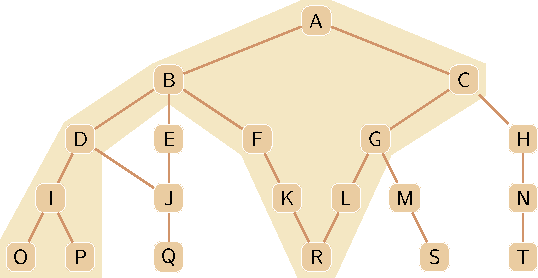
\includegraphics[page=1]{images/simgic.pdf}}
    \subbottom[
        The induced graph for an entity annotated with concepts \term Q, \term R, \term S and~\term T.
        \label{fig:induced-graph/e'}
    ]{\includegraphics[page=2]{images/simgic.pdf}}
    
    \caption[Group-wise measures in action]{Two entities, annotated with a set of concepts form a toy ontology, are being compared using the idea of the induced graph. The figures show the ontology concepts and the class-subclass hierarchy, as well as the induced graph for the two entities in a shaded background.}
    \label{fig:induced-graph}
\end{figure}

Consider the toy ontology in \figref{fig:induced-graph} and two entities: $e$~is annotated with the set~$\{\term O,\term P,\term R\}$ and~$e'$ with the set~$\{\term Q,\term R,\term S,\term T\}$. The induced graphs of $e$ and~$e'$ are shown in the shaded regions of the graphs in \figref{fig:induced-graph/e} and \figref{fig:induced-graph/e'}, respectively. In this example, we have:
\begin{eqnarray*}
    \phi(e) \cap \phi(e') &=& \{\term A,\term B,\term C,\term D,\term F,\term G,\term K,\term L,\term R\} \\
    \phi(e) \cup \phi(e') &=& \{\term A,\term B,\term C,\term D,\term E,\term F,\term G,\term H,\term I,\term J,\term K,\term L,\term M,\term N,\term O,\term P,\term Q,\term R,\term S,\term T\}
\end{eqnarray*}
Using Seco's intrinsic measure of information content from \eqref{eq:seco}, we get, for example, $\IC(\term B) = 1 - \frac{\log 11}{\log 20}=0.20$; and through \eqref{eq:simui,eq:simgic}, we can compute the similarity between the two entities:
\begin{eqnarray*}
    \sim[UI](e,e')  &=& 0.45,\\
    \sim[GIC](e,e') &=& 0.34.
\end{eqnarray*}

Besides this type of measure, where the sets of annotations are directly compared to each other, there are group-wise measures that are built over concept-wise measures. Let $e_1,e_2,\ldots$ be the concepts that annotate a certain entity~$e$. To compare two entities $e$ and~$e'$ in this case, all the pairs $(e_i,e'_j)$ are compared using the concept-wise measure, creating a similarity matrix which is then converted into a single value. For example, the average over all the similarities and the maximum of these values are used in the literature~\citep{Lord2003,Grego2010}.

Another way of aggregating the matrix is the Best Match Average (BMA). This method goes through each of the $e_i$~concepts and finds the annotation in~$e'$ that is most similar to it, and then goes through each of the $e'_j$~concepts and finds the annotation in~$e$ that is most similar to it. The result is the average of all these maximum values~\citep{Wang2007,Pesquita2008,Grego2010}. Assuming $e$ has $n$~annotations and $e'$ has $m$~annotations:
\begin{equation}
    \sim[BMA](e,e') = \frac{
        \sum_{i=1}^n \max_{j} \sigma(e_i, e'_j) +
        \sum_{j=1}^m \max_{i} \sigma(e_i, e'_j)
    }{n + m}
    \label{eq:bma}
\end{equation}
where $\sigma$~is a concept-wise similarity measure (it takes as input two concepts).

\figref{fig:bma} illustrates this process using the same two entities that were used in the previous example. The similarity matrix, calculated with $\sim[Resnik]$~(\eqref{eq:resnik-ssm}) and $\IC[Seco]$~(\eqref{eq:seco}), is shown in the depicted matrix, and the maximum values for each row and column are extracted (see the arrows in the picture) and averaged:
\begin{eqnarray*}
    \sim[BMA](e,e') = 0.42. \label{eq:bma-e-e'}
\end{eqnarray*}

\citet{Lehmann2012a} suggest a further enhancement to this formula. One of the issues of BMA is that it only takes into account one annotation in~$e'$ for each annotation in~$e$, specifically \emph{the most} similar one. However, it can be the case that, for some~$i$, $e_i$~is extremely similar to two or more $e'_j$. Instead of extracting just the maximum similarity value in each row or column, they propose the use of a T-conorm~\citep{Klement2004} to aggregate all the values. T-conorms are binary operations (commonly represented as~$x \oplus y$) that satisfy a set of properties, the most important of which, in this context, being $\max(x,y)\leq x \oplus y \leq 1$. As such, it is possible to take into account more than just one most similar concept and to use the \emph{trend} of concept similarity in order to calculate the similarity between the annotated entities.

For example, we can use $x \oplus y = x + y - xy$. Taking into consideration not just one value in each row\slash column of the matrix, but rather two values, we reach the situation described in \figref{fig:bma-tconorm}, where each row (\emph{resp.}~column) is aggregated to reach a final score that depends on the two highest values in that row (\emph{resp.}~column). In this case, we would have
\begin{eqnarray*}
    \sim[BMA'](e,e') = 0.51, \label{eq:bma-tconorm-e-e'}
\end{eqnarray*}
which is slightly larger than the previous calculation in \eqref{eq:bma-e-e'}, because we are now taking into consideration more similarity values. This strategy produces higher values, where the increase depends on the overall trend followed by the similarity values of the matrix. For example, a matrix composed entirely of $0$s and~$1$s will produce an identical value using the BMA approach or this one.

\begin{figure}
    \centering
    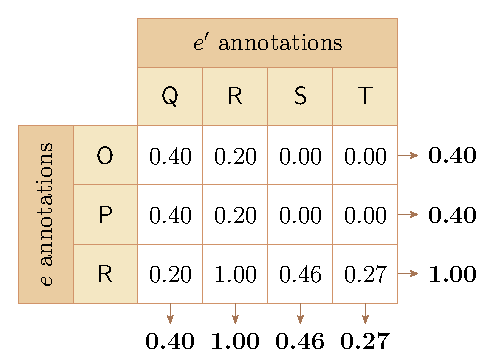
\includegraphics{images/bma.pdf}
    \caption[Example of the best match average in action]{Using the same entities referred to in \figref{fig:induced-graph}, this picture represents the best match average approach. Values in the matrix are the semantic similarity between the corresponding concepts, calculated with $\sim[Resnik]$ and $\IC[Seco]$. The arrows pointing to bold values show the maximum of each row and column, and the final result is the average of those maximum values.}
    \label{fig:bma}
\end{figure}

\begin{figure}
    \centering
    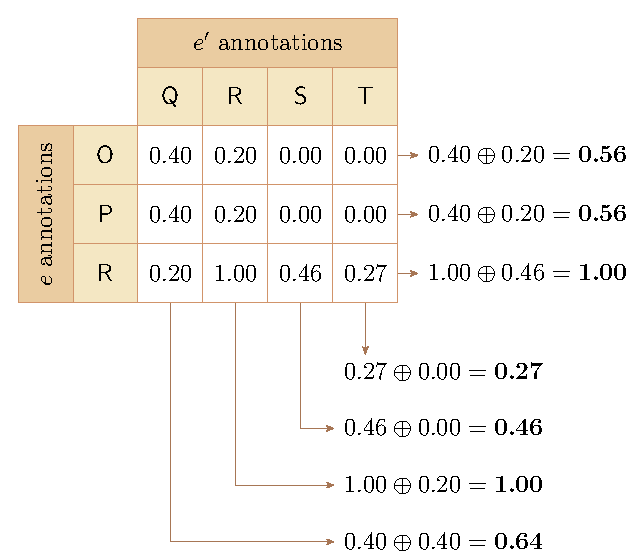
\includegraphics{images/bma-tconorm.pdf}
    \caption[The T-conorm aggregation strategy]{This figure illustrates the use of the T-conorm $x \oplus y = x + y - xy$. This strategy uses the two highest values from every row and every column to derive a single value for the annotations in each of the two entities, rather than using only the highest.}
    \label{fig:bma-tconorm}
\end{figure}


\section{Multiple-ontology semantic similarity} \label{sec:sota/multi-ontology}

At the time of this document, and to the best of my knowledge, there is no published work dealing with semantic similarity in multi-domain contexts. Measures used in the literature are either single-ontology or multiple-ontology single-domain (see \secref{sec:concepts/multi-ontology}) that use ontologies representing distinct perspectives of a single domain in order to enrich the similarity between the concepts of that domain. These studies are usually applied to the Systematized Nomenclature of Medicine ``Clinical Terms''(\ontology{SNOMED-CT})~\citep{Cote1980}, Medical Subject Headings (\ontology{MeSH})~\citep{Rogers1963} \andor WordNet~\citep{Miller1995}.

While the absence of approaches in this area means that my own measures of multi-domain similarity will have nothing to be compared with, the multi-ontology single-domain approaches provide interesting insight into the issues of integrating multiple ontologies in a single measure of similarity and how to solve them.

These measures of similarity have been first approached by \citet{Rodriguez2003}. Similarity measures that cross different ontologies rely on links between the concepts of the ontologies, meaning that it is vital that such links exist. The authors use lexical similarity to find these matches. While this is a weak form of ontology matching (for example, the lexical similarity between \term{Role} and \term{Activity} is~$0$ by most \mdash if not all \mdash intuitive lexical similarity measures, despite the fact that they are related concepts in chemistry), the use of synonymy enriches this measure. Semantic similarity is then calculated based on the class-subclass hierarchy of the concepts in the set of used ontologies, taking the links found in the previous step into account.

\citet{Al-Mubaid2009} propose an edge-based semantic similarity that also crosses ontologies. To do so, they introduce the notion of \emph{primary ontology}: all similarities are calculated based on a scale that is balanced for the primary ontology. They use an edge-based measure and scale the edge distances of secondary ontologies according to the difference in maximum depth between the primary and secondary ontologies. The specificity of a concept, measured by its depth, is also appropriately scaled. Their similarity is then defined as
\begin{equation}
    \sim[AlMubaid] = \log \left(
        \left(p(a,b)-1\right)^\alpha\cdot c_s(a,b)^\beta + k
    \right)
    \label{eq:almubaid}
\end{equation}
where $p(a,b)$~is the scaled length of path between concepts $a$ and~$b$ (which may cross ontologies by means of the inter-ontology links), $c_s(a,b)$~is the scaled depth of the LCS between $a$ and~$b$, and $\alpha$, $\beta$ and~$k$ are tunable parameters of the measure.

\citet{Sanchez2012c} define an approach that uses the notion of \emph{semantic overlap}, which measures the overlap in the hyponyms of each concept:
\begin{equation}
\mathrm{overlap}(a^P,b^Q) =
\frac{|H^P(a^P)\cap H^Q(b^Q)|}
         {\sqrt{|H^P(a^P)|\times|H^Q(b^Q)|}}
\label{eq:sanchez-hyponyms}
\end{equation}
where $c^O$~is used to represent the concept~$c$ in ontology~$O$ and $H^O(c^O)$~is the set of hyponyms of the concept~$c^O$ in ontology~$O$. This overlap is calculated through lexical methods, as in the work of \citet{Rodriguez2003}.

\citet{Sanchez2013} extend the notion of information content to the multiple-ontology context, by defining the MICA of two concepts when
\begin{paralist}
    \item the two simultaneously belong to two or more ontologies; or
    \item there is no ontology that contains both concepts.
\end{paralist}
This redefinition of the MICA is then used in the original formulas by \citet{Resnik1995}~(\eqref{eq:resnik-ssm}), \citet{Lin1998}~(\eqref{eq:lin}), \etc.

As is evident from these works in multiple-ontology single-domain semantic similarity, using multiple ontologies to calculate similarity is a process that strongly depends on links between the ontologies. These can come from previous alignments produced by ontology matching techniques~\citep{Euzenat2007} or can be calculated \emph{on-the-fly} by using lexical algorithms coupled with sets of synonyms. The recent advances in ontology matching, especially in the biomedical field \citep[\eg][]{Cruz2009a,Gross2012}, represent a big step forward in the determination of equivalent concepts between ontologies.

Given the ontology interoperability that is highly sought in the biomedical informatics community (see the last paragraph in \secref{sec:concepts/ontologies}), it is expected that concepts from two different ontologies never represent the same real-world idea. As such, ontology matching does not seem to be as useful in the context of multi-domain similarity as it is in single-domain similarity.

In contrast, what \emph{is} necessary and useful is the notion of inter-domain links between concepts that are related. Some biomedical ontologies already make cross-references from its concepts to concepts from other ontologies~\citep{Kamdar2015}. For example, \ontology{HPO}, an ontology of human phenotypes, makes use of concepts from other ontologies to define their own concepts: \eg the definition of \term{Asymmetry of the mouth} makes reference to the concepts \term{Asymmetric} from \ontology{PATO} and \term{Mouth} from \ontology{FMA}. These links, rather than the ones between equivalent concepts, are likely to be useful in my endeavour.


\section{Recent advances} \label{sec:sota/recent}

As a community, we are now empowered with tools that allow us to compare concepts and annotated entities, using methods known to work in different scenarios. Consequently, the amount of new semantic similarity measures being proposed has been decreasing. Instead, there have been different types of advances in this field of research. Recent literature tries to
\begin{paralist}
    \item systematise and organise this field, so that future research can be even more powerful; and
    \item use the already existing measures in ways that can improve their already high performance.
\end{paralist}

\citet{Harispe2014} present a framework that tries to contribute to the understanding of semantic measures by unifying the existing measures into a single theory of semantic similarity, citing at least $21$~different concept-wise measures, proposed from 1989 to~2012, and how they fit into their framework.

In one of my contributions (see \secref{sec:enhancements/disjointness}), I have also proposed and validated a new measure of shared information content to use in the chemical domain~\citep{Ferreira2013}. Again, this is not a new measure of similarity but a \emph{plug-in} that can be incorporated in existing measures in order to take into account different ontology constructions (in this case, disjointness axioms).

This document falls under the scope of these new research endeavours, since, as we will see in \chpref{chap:multidomain}, I do not propose a mutli-domain measure of similarity from scratch, but build it as a set of extensions that are based on already existing measures enabling their application on entities annotated with concepts from more than one ontology.


\section{Summary and classification} \label{sec:sota/summary}

The current measures of semantic similarity can be classified according to four axes:
\begin{description}
    \item[Extension] Measures that use only the information contained in the ontologies representing the concepts being compared are \emph{intrinsic}, while the ones that use external resources are \emph{extrinsic}.
    
    \item[Source of semantics] Measures can be \emph{edge-based} or \emph{node-based}. They can also use other attributes of a concept, namely their labels or synonyms, which are \emph{lexical} sources of semantics. Using information content measures to calculate the specificity of a concept is also possible for node-based measures.
    
    \item[Ontology multiplicity] Measures can be \emph{single-ontology}, \emph{multiple-ontology single-domain} and \emph{multi-domain}. Given the absence of multi-domain measures in the literature, only single-ontology and multiple-ontology single-domain measures have been described.
    
    \item[Aggregation technique] Group-wise measures that are based on concept-wise measures must use a technique to aggregate the similarity matrix into a single value. The techniques explored in this chapter are the \emph{average} of the matrix, the \emph{maximum} and the \emph{best match average} (BMA). Some group-wise measures are not based on concept-wise measures (\eg $\sim[UI]$ and~$\sim[GIC]$).
\end{description}

As a summary of this whole chapter, \tabref{tab:summary-ssm} classifies all the mentioned measures based on these four axes.

\begin{table}

% Define short-cuts for the table
\def\int{intrinsic}
\def\ext{extrinsic}
\def\intext{\int\ \& \ext}

\def\e{edges}
\def\n{nodes}
\def\ic{$^\textrm{IC}$}

\caption[Summary of the characteristics of some semantic similarity measures]{Node based measures that use the notion of information content to calculate specificity are marked with \ic. Concept-wise measures do not have an aggregation technique and, as such, are marked with a dash (--) in that column. SO: single ontology; MO: Multi-ontology single-domain; BMA: best match average; GW: Group-wise measure not based on a concept-wise measure.}
\label{tab:summary-ssm}

\centering
\small
\begin{tabular}{lllll}
\toprule
\bfseries Publication &
\multicolumn{4}{l}{\bfseries The four axes of classification} \\
\cmidrule{2-5}
  & Extension & Source of & Ontology     & Aggregation \\
  &           & semantics & multiplicity & technique   \\
\midrule
\citep{Rada1989}      & \int    & \e             & SO & --          \\
\citep{Wu1994}        & \int    & \e             & SO & --          \\
\citep{Resnik1995}    & \ext    & \n\ic          & SO & --          \\
\citep{Jiang1997}     & \ext    & \n\ic          & SO & --          \\
\citep{Lord2003}      & \ext    & \n\ic          & SO & average     \\
\citep{Rodriguez2003} & \int    & \n\ \& lexical & MO & --          \\
\citep{Seco2004}      & \int    & \n\ic          & SO & --          \\
\citep{Clemente2005}  & \int    & \e\ \& \n\ic   & SO & adapted BMA \\
\citep{Lei2006}       & \int    & \e             & SO & various     \\
\citep{Gentleman2007} & \int    & \n             & SO & GW          \\
\citep{Couto2007}     & \ext    & \n\ic          & SO & --          \\
\citep{Wang2007}      & \int    & \n             & SO & BMA         \\
\citep{Pesquita2008}  & \ext    & \n\ic          & SO & GW          \\
\citep{Al-Mubaid2009} & \int    & \e             & MO & --          \\
\citep{Kohler2009}    & \ext    & \n\ic          & SO & BMA         \\
\citep{Schlicker2010} & \ext    & \n\ic          & SO & BMA         \\
\citep{Ferreira2010}  & \ext    & \n\ic          & SO & --          \\
\citep{Grego2010}     & \ext    & \n\ic          & SO & BMA         \\
\citep{Couto2011}     & \intext & \n\ic          & SO & --          \\
\citep{Sanchez2011e}  & \int    & \n\ic          & SO & --          \\
\citep{Batista2012}   & \ext    & \n\ic          & SO & --          \\
\citep{Sanchez2012b}  & \int    & \n             & SO & --          \\
\citep{Sanchez2012c}  & \int    & \n             & MO & --          \\
\citep{Sanchez2013}   & \intext & \n\ic          & MO & --          \\
\bottomrule
\end{tabular}

\end{table}




\part{Contributions}
\epigraph{Scientists have become the  bearers of the torch of discovery in our quest for knowledge.}{Stephen Hawking}

\chapter{Validation strategies} \label{chap:validation}

\begin{note-paper}
    This chapter is adapted from one of my papers, submitted to the Journal of Biomedical Semantics on September 2015 and still waiting a review.
\end{note-paper}

One vital step in the development of semantic similarity algorithms is their validation. This step assesses the accuracy of the proposed measure with respect to a predefined goal. As such, choosing the correct validation strategy is vital to ensure the scientific soundness of the results obtained with semantic similarity: a biased or inappropriate validation strategy can erroneously certify the similarity measure and, in the worst case, lead to the validation of wrong conclusions and incorrect facts.

However, despite the importance of this step, validation of semantic similarity measures is usually carried out in an \emph{ad-hoc} manner, with no systematization having ever been conducted around this subject. Such a systematization is important to all intervening parties (developers of semantic similarity, users of these measures, and scientific literature publishers) because:
\begin{itemize}
    \item it provides semantic similarity developers a way to choose a validation strategy that is appropriate for their measure and its application end-goals;
    \item it exposes the differences and resemblances between validation strategies, thus enabling developers to choose one that is orthogonal to the ones already executed;
    \item it empowers users to more quickly ascertain whether the validation strategy that was used to evaluate a measure is relevant for their use cases and, by extension, whether the measure itself is appropriate for their goals; and
    \item it allows a standardisation of validation strategies: the existence of a controlled vocabulary that encodes the domain of validation strategies enables both developers and literature publishers to annotate their works with the classes within this hierarchy, enhancing the accuracy of metadata associated with publications.
\end{itemize}

The last item above is in accordance with the practices of semantic web (see \secref{sec:concepts/semantic-web}), and can one day allow techniques such as semantic similarity itself to be applied on scientific literature as much as it is currently on scientific data, hence contributing to data mining and to information retrieval in general.

Realising these advantages and the lack of a proper classification of validation strategies for semantic similarity measures, I decided to contribute by assessing which strategies have been reported in literature. During the work I carried out for this PhD, I came across a vast collection of semantic similarity measures proposed in several contexts and, as such, I am acquainted with the many strategies used to validate them. However, a scientific systematization rests on a reproducible methodology that can be carried out by anyone, irrespective of their past experience in the area. As such, I developed a method for systematically classifying validation strategies based on a literature review.

The first step was to narrow the whole semantic similarity domain. Given the popularity of \ontology{GO}, semantic similarity measures have been extensively proposed and studied using this ontology as a source of knowledge, and only a few works have been published that propose semantic similarity in other biomedical ontologies. As such, the systematization of validation strategies was done based on \ontology{GO} semantic similarity alone. This decreased the amount of literature that had to be checked but did not significantly reduce the amount of validation strategies that have been found. In this sense, the hierarchy that was created is generic on the domain of application, but contains at the moment only validation strategies found with \ontology{GO}-based measures. In theory, the strategies that I encountered in the literature review can be adapted and followed to validate semantic similarity in other ontologies \mdash for example, I have previously validated semantic similarity in \ontology{CHEBI} by comparing it with structural similarity~\citep{Ferreira2010,Ferreira2013}; \ontology{HPO} similarity has been validated by determining whether the measure can predict diseases based on phenotypes~\citep{Kohler2009}. Several facts contributed to my choosing \ontology{GO} over the other ontologies:
\begin{itemize}
    \item It was one of the first biomedical ontologies to have been used in ontology-based semantic similarity measures~\citep{Lord2003}, and has since been extensively used with this purpose throughout the years (it is probably \emph{the most} extensively used).
    
    \item It is also a formal ontology. \ontology{GO} is written in both OBO and OWL; therefore, it uses the first-order logic constructions that these languages provides to represent knowledge. This is in contrast with other highly used vocabularies which use instead generic and underspecified properties between concepts, such as \ontology{MeSH} or \ontology{SNOMED-CT} (see some examples in \secref{sec:concepts/ontologies}).
    
    \item \ontology{GO} is in an advanced stage of development. It was the first biomedical ontology to have been developed with an objectively defined domain rather than being a general purpose vocabulary, and it is used extensively amongst the computational biology and bioinformatics communities to annotate gene products (proteins and other molecules derived from DNA that serve a function in the cell).
    
    \item Similarity measures between proteins have many different applications, including
    \begin{paralist}
        \item transferring knowledge between proteins~\citep{Tao2007} (\eg by comparing a protein with other proteins, one can predict unknown functions by hypothesising that similar proteins have similar functions);
        \item predicting whether two proteins interact~\citep{Azuaje2004,Guo2006} (either physically, by forming a complex, or in less obvious ways, like being part of the same metabolic pathway); and
        \item automatically categorising a collection of proteins in meaningful groups to facilitate future research in finding proteins of interest~\citep{Doms2005}.
    \end{paralist}
    While protein similarity has been traditionally performed by resorting to their amino-acid sequence, with methods such as BLAST~\citep{Altschul1997} and the Smith-Waterman algorithm~\citep{Smith1981} being associated with highly relevant results in knowledge transfer~\citep{Wyman2004}, semantic similarity has become a tool of its own, having contributed to the aforementioned tasks.
\end{itemize}


\section{Methodology} \label{sec:validation/methodology}

Having selected \ontology{GO} as the target ontology for this classification endeavour, I developed a reproducible methodology:
\begin{enumerate}
    \item On May 21\textsuperscript{st} 2015, I conducted a search using the PubMed bibliographic database with the query \texttt{"semantic similarity" "gene ontology"}. This resulted in $121$~articles being retrieved.
    \item An empty set of validation strategy classes was initialised.
    \item For each of the $121$~articles, I read the abstract and extracted from it the validation strategies that were followed. When the abstract was insufficient to perform this step, I read instead the full text, when available.
    \item Each validation strategy was classified under one of the classes in the set or, if no appropriate class existed, a new one was created. \label{item:classification}
    \item Finally, the classes found in the previous step were organised in a hierarchical structure.
\end{enumerate}

Step~\ref{item:classification} is the most relevant for this task, but it is also susceptible to some subjectivity, as the classification of the measures may not always be straightforward. For example, a new strategy may be slightly different from a previously encountered one, and it is not always obvious if a new class should be created or if the two strategies should instead be classified with the same class. To minimise this subjectivity, whenever a new class is inserted in the set for this reason (\ie when a more specific version of an existing strategy is found), all the strategies previously classified under that class were reassessed.

Only papers that validated semantic similarity were considered. Hence, I filtered papers that use semantic similarity as part of another system, whose main purpose is \emph{not} the comparison of gene products, \eg papers that introduce a methodology that uses semantic similarity to support protein-protein interaction queries~\citep{Guzzi2013} or to find patterns in genome-wide associated studies~\citep{Kim2013}.


\section{A hierarchy of validation strategies} \label{sec:validation/hierarchy}

The main result of this task was the hierarchy created during the literature review process. \figref{fig:hierarchy} summarises the strategies that were found by following the methodology above. The hierarchy classifies validation strategies into four main branches (represented by a grey shade in the figure), each one further divided into more specific types of validation strategies. The numbers on the right indicate the amount of papers that use a validation strategy of that type, both directly and indirectly (for example, no strategy was classified directly as ``Contextual behaviour'', but instead I classified papers with the leaves under that branch).

\begin{figure}
    \centering
    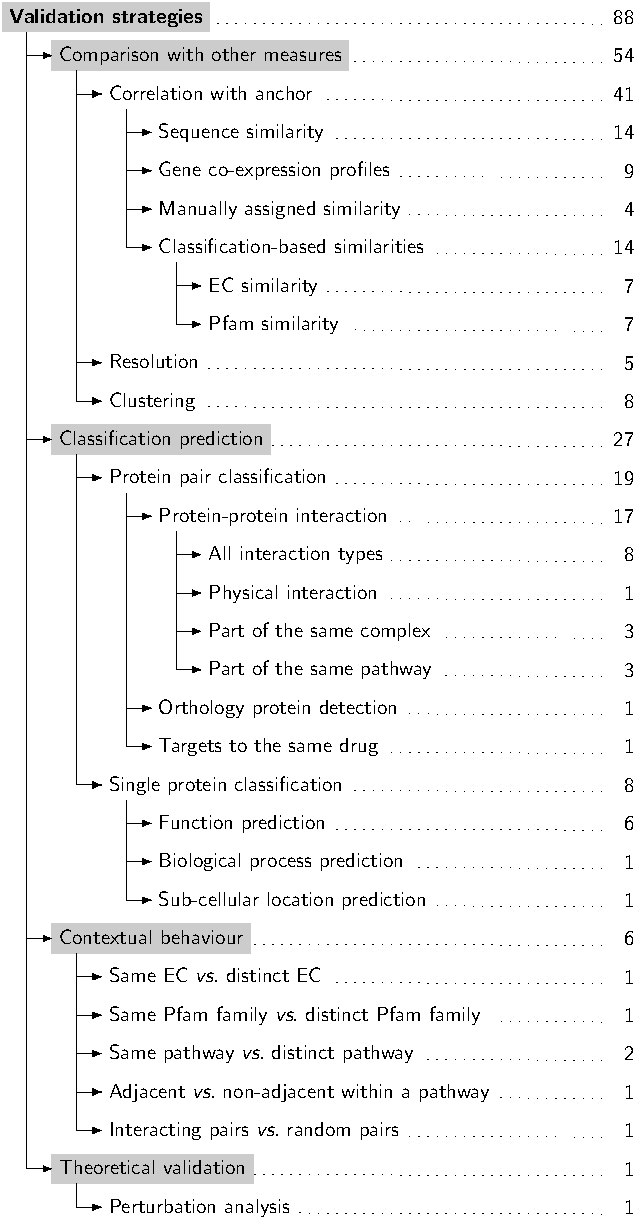
\includegraphics[height=0.8\textheight]{images/hierarchy.pdf}
    \caption[Hierarchy of strategies employed in \ontology{GO}-based similarity validation]{The column on the right contains the number of strategies found in literature that were classified with the corresponding class, either directly or indirectly. The only non-leaf strategy that has been used to classify a strategy is \term{Protein-protein interaction}, which correspond to works that use unspecified types of protein-protein interaction.}
    \label{fig:hierarchy}
\end{figure}

The validation strategy hierarchy produced in this task contains four branches, which can be defined as follows:
\begin{description}
    \item[Comparison strategies] The semantic similarity measure is compared to another similarity measure, which I name the \emph{anchor}. This comparison is supported by a dataset that includes the \emph{anchor} similarity values for pairs of proteins.
    
    \item[Classification strategies] The semantic similarity measure is used as the basis for a classification model (through machine-learning algorithms) which is trained to predict a certain property of gene-related entities (\eg proteins or pairs of proteins).
    
    \item[Contextual validation] Semantic similarity is calculated for two kinds of protein pairs, which are hypothesised \emph{a priori} to exhibit different similarity patterns (\eg proteins that interact with one another should show higher similarity values than random protein pairs). Statistical methods are used to show that similarity in one of the groups is indeed, on average, higher than in the other group.
    
    \item[Theoretical validation] The semantic similarity values alone are used as validation, providing a ``sanity check'' over the semantic similarity measure, rather than an actual validation using real-world data.
\end{description}

The next subsections detail the various strategies included in the hierarchy.


\subsection{Comparison with other measures} \label{sub:hierarchy/comparison}

One of the most straightforward ways to determine the performance of a semantic similarity measure is to compare it with an anchor measure to determine how well semantic similarity reflects the anchor (\eg by determining the Pearson's correlation coefficient between the two measures). There are two main scenarios where it is desirable to apply this strategy:
\begin{itemize}
    \item The anchor measure may take a long time to perform and may not be scalable for large and rapidly changing datasets. This is the case of manual similarity values assigned to pairs of proteins by experts: manual comparison is not practical for real-time systems, such as the search functionality in a protein database.
    \item The anchor measure may have already been proven successful for a certain task. In this case, deploying a new measure that highly correlates with the old one provides a good argument in favour of the suitability of the semantic measure at least in the same task. For example, sequence similarity can be used to predict protein sub-cellular localization~\citep{Nair2002}. Furthermore, a single similarity measure that highly correlates with several anchor measures, each developed to suit a specific task, can be regarded as a generalization of those measures.
\end{itemize}

A note of warning is needed when considering these strategies: perfect correlation is not the end goal. In fact, devising a new measure that is completely aligned with an old one can be considered a mere academic exercise, as no information can be extracted from the new measure that could not have been inferred from the anchor. The only advantage is if the new measure takes less time or less memory to compute, or if it does not depend on extra knowledge sources; usually, however, semantic similarity is slow (compared to other algorithms) and uses external information in its intermediate calculations.

Additionally, automatic anchor measures are usually known to have some shortcomings. For example, sequence similarity has been notoriously used for a few decades under the assumption that similar amino-acid sequences often correspond to similar functions \citep[\eg][]{Bork1998}; but that assumption fails in some cases, such as similar sequences corresponding to disparate functions, or similar functions being performed by proteins with completely different sequences~\citep{Whisstock2003,Watson2005}. As such, it is important to clearly state that, even though a high correlation with an anchor measure is an argument for the suitability of the new measure, care must be taken when interpreting actual correlation coefficients between semantic and other non-manual similarity measures.

Correlation strategies differ essentially on the anchor measure they use:
\begin{description}
    \item[Sequence similarity measures] These assign a numeric value to a pair of proteins based on their amino-acid sequences. Sequence similarity measure used in these validation strategies are based on Smith-Waterman~\citep{Smith1981} and BLAST~\citep{Altschul1997}.
    
    \item[Gene co-expression profiles] The expression levels of two genes are compared in several different situations, and the absolute value of Pearson's correlation coefficient between the expression values throughout these situations is measured. Based on the assumption that similar genes exhibit similar expression levels in the same situation (\ie they present a high overlap in their expression profiles), a high correlation between their expression profiles and the semantic similarity between the pair is used to validate the measure~\citep[\eg][]{Wang2004,Jain2010,Yang2012}.
    
    \item[Manual similarity] Sometimes, it is possible to have an expert go through a series of pairs of protein or pairs of \ontology{GO} concepts and assign each one a similarity value, which the semantic similarity measure must reflect~\citep[\eg][]{Xu2013}.
    
    \item[Classification-based similarity] Automatic similarity derived from the manual classification of the proteins has also been used. One example is the use of the Enzyme Commission~(EC) classification~\citep{Moss2015} to compare two enzymes (the similarity is the number of levels in the two EC numbers that match); this strategy was introduced by~\citet{Pesquita2009a}. Another example is the Pfam classification~\citep{Bateman2002} (similarity is the number of shared families between the two proteins); this validation strategy was introduced by~\citet{Couto2007}.
\end{description}

Another way to determine the performance of a semantic similarity measure is to calculate its \emph{resolution} with respect to the anchor measure, a numeric value that reflects the overall behaviour of the measure. This evaluation was first introduced by~\citet{Pesquita2008}, and is defined as ``the relative intensity with which (on average) variations in the sequence similarity scale are translated into the semantic similarity scale''. The assumption is that the higher the resolution, the more accurate is the semantic similarity measure, as it can reflect small differences in two proteins that a measure with less resolution cannot.

The final strategy in this branch consists in using the semantic similarity measure to cluster proteins and then compare the resulting cluster with a reference, which may be manually assembled or can itself be based on other resources. \citet{Wang2007} validate semantic similarity by manually assessing whether the results of hierarchical clustering reflect an expert notion of clustering. Automatic alternatives to this include the Davies-Bouldin Index~\citep{Davies1979} or the Fowlkes-Mallows Index~\citep{Fowlkes1983}, which measure the degree to which two clustering results overlap.


\subsection{Classification strategies} \label{sub:hierarchy/classification}

Semantic similarity can also be validated by assessing whether it can predict properties of proteins or protein pairs. For these strategies, a dataset of known property values must be given in advance (the ``gold-standard''), and the validation strategy usually consists in determining some kind of accuracy of the semantic similarity measure in predicting these properties.


\subsubsection{Protein-protein interactions}

The most straightforward way of basing classification problems on semantic similarity values is to use the similarity between two proteins to predict whether they interact. Interaction, in this context, can be interpreted as:
\begin{itemize}
    \item the actual physical, momentary interaction between the proteins, such as when one of the proteins modifies the other protein (\eg through phosphorylation);
    \item the long-lived interaction between proteins that are part of the same multi-protein cluster (\eg ribosomes consist of a series of proteins and, thus, form a multi-protein complex); and
    \item a more abstract notion of interaction that occurs when the two proteins are part of the same metabolic pathway (\eg they both regulate the same process).
\end{itemize}

In these classification problems, a dataset of positive pairs is provided containing pairs of proteins that are known to interact. Negative pairs can be gathered from the literature (\eg from journals such as the Journal of Negative Results in Biomedicine) or randomly generated. Furthermore, random generation can be
\begin{paralist}
    \item blind, \ie any pair is accepted in the set; or
    \item generated in such a way that it is known to contain few positive pairs.
\end{paralist}
This last method can drastically reduce the chances that a positive pair ends up in the negative dataset. For example, since proteins that are part of the same cluster must necessarily coexist in the same cellular location, the generation of negative pairs may exclusively generate pairs of proteins that are known to be located in separate cell compartments. However, \citet{Ben-Hur2006} argue that building the negative set in this way can lead to unreliable performance indicators, because there are proteins in the same cellular compartment that are not, in fact, part of the same complex. Thus, this selection method introduces a bias.

\tabref{tab:ppi} describes some of the validation strategies that were found in the literature review and that were classified under ``Protein-protein interaction''. All the strategies use some sort of online biomedical database to create the positive dataset, while generally the negative dataset is randomly constructed. Several types of interaction can be used, even within the same strategy, and the performance is usually reported
\begin{paralist}
    \item as some statistical test (for example, the \emph{p}-value associated with the capacity of the measure to predict the correct interactions),
    \item as the value of precision, or
    \item as the value of the Area Under the Curve (AUC) of a Receiver Operating Characteristic curve~\citep{Fawcett2004,Fawcett2006}.
\end{paralist}

Several datasets typically used by these strategies include:
\begin{itemize}
    \item KEGG, the Kyoto Encyclopedia of Genes and Genomes~\citep{Ogata1999}, can be used to find proteins that participate in the same pathway or that are part of the same protein complex;
    \item CORUM~\citep{Ruepp2008} is a dataset of mammal protein complexes; and
    \item DIP~\citep{Salwinski2004} is an all-purpose interaction database, containing at least $28$~different protein-protein interaction types.
\end{itemize}


\begin{table}
    \caption[Protein-protein interaction validation strategies]{This table shows the details of representative instances of validation strategies based on protein-protein interaction prediction. Each strategy can have more than one data source to construct the positive and negative pairs of the dataset, as well as using multiple interaction types and performance measures.}
    \label{tab:ppi}
    
    \centering
    \small
    \def\paper#1{\midrule \citep{#1} }
    
    \begin{tabular}{lllll}
    % headers
    \toprule
    \textbf{Paper} &
    \multicolumn{2}{c}{\textbf{Dataset}} &
    \textbf{Interaction type} &
    \textbf{Performance} \\
    
    \cmidrule{2-3}
      & \itshape positive pairs & \itshape negative pairs \\
    
    % content
    \paper{Azuaje2004}
      & custom dataset & custom dataset & same complex & statistical test \\
    \paper{Guo2006}
      & \kegg{Pathway}, & random         & same pathway, & AUC, \\
      & \kegg{Module},  &                & same complex  & statistical test, \\
      & BIND            &                &               & precision \\
    \paper{Jain2010}
      & DIP             & random         & physical,     & AUC \\
      &                 &                & same pathway \\
    \paper{Mathur2012}
      & \kegg{Pathway}  & \kegg{Pathway} & same pathway  & statistical test \\
    \paper{Yang2012}
      & CORUM           & random         & same complex  & AUC \\
    \paper{Vafaee2013}
      & I2D, Reactome   & random         & physical,     & AUC \\
      & KEGG, NetPath,  &                & same pathway, \\
      & NCI-PID,        &                & same complex  \\
      & CORUM \\
    \bottomrule
\end{tabular}

\end{table}

\subsubsection{Orthology detection}

Another property of protein pairs that can be predicted by using semantic similarity is the implicit property that exists between orthologous proteins. The main assumption of this strategy is that orthologs (\ie proteins whose genes are, in evolutionary terms, descendent of the same ancestral DNA sequence) should exhibit a higher similarity than other pairs of proteins. \citet{Wu2013} introduced this idea and used a statistical test to validate semantic similarity by noticing that the similarity values between orthologous proteins is higher than between random protein pairs.


\subsubsection{Single protein property prediction}

While classification problems involving protein pairs are the most common, there are validation strategies directed at the properties of individual proteins as well. Three such examples have been found in the literature: prediction of protein function, prediction of the biological processes in which the protein participates, and prediction of sub-cellular localization. These three prediction problems map directly to the three \ontology{GO} branches: molecular function, biological process and cellular component. In fact, these strategies can be rephrased as follows:
\begin{quote}
    Given a set of \ontology{GO} annotations, predict new annotations to go along with them.
\end{quote}
This is a way of \emph{enriching} an annotation set with more concepts.

In these strategies, semantic similarity between the protein whose property is being predicted and the proteins whose property value is already known is used as part of a machine-learning strategy. As such, the training dataset must already contain the known property values: \eg the training dataset for the function prediction problem must contain a set of proteins and their actual function(s). Performance is reported using measures frequently used in machine-learning, such as the accuracy of the machine-learning algorithms, or the AUC of the corresponding ROC curve.


\subsection{Contextual behaviour} \label{sub:hierarchy/contextual}

Like the strategies of the previous branch, ``contextual behaviour'' strategies are based on the assumption that proteins that are in some way related should exhibit a higher similarity (in general) than the ones where that relation does not hold. However, instead of predicting properties of proteins, these methods consist in only observing whether that assumption holds. For example, proteins that are adjacent in a certain metabolic pathway should exhibit higher average semantic similarity than proteins of that pathway that are not adjacent.

In order to prove that this behaviour holds, statistical methods are frequently used to show that average semantic similarity in one of the groups is statistically higher in the other group, which can be achieved using, \eg \hbox{$Z$-test} or Student's~\hbox{$t$-test}~\citep{Rosner2010}.

Strategies found in the literature search include dividing protein pairs depending on whether the two proteins:
\begin{itemize}
    \item have the same EC classification;
    \item have the same Pfam family;
    \item participate in the same metabolic pathway;
    \item are adjacent or non-adjacent within a metabolic pathway; or
    \item form a known protein-protein interaction.
\end{itemize}

It must be noted that these strategies are not technically much different from the use of an anchor measure. For example, we could create an anchor measure that assigns $1$~to protein pairs where the two proteins have the same EC classification and $0$~to other protein pairs, and then correlate this measure to semantic similarity. However, anchor measures tend to be continuous rather than categorical (they return a real number in a range, usually between $0$ and~$1$). Furthermore, in contextual behaviour strategies, the goal is to determine whether we can observe a statistically significant difference between the semantic similarity in one group with respect to another group, rather than to calculate a correlation coefficient.


\subsection{Theoretical validation} \label{sub:hierarchy/theoretical}

Theoretical validation strategies depend only on the actual semantic similarity values between pairs of proteins and not on any other information about those pairs.

The only validation instance I encountered in this branch was the calculation of the ``resistance to ontology perturbation''~\citep{Mathur2012}. This strategy measures how much the semantic similarity values change when the ontology underlying the measure is changed. Being robust to perturbation is regarded as a necessary condition for a useful similarity measure, as ontologies change over time and the (usually) small variations from one version to the next should not have a significant impact on the similarity values calculated between proteins. For a robust measure, increasing perturbation rates cause increasing deviation. In a non-robust measure, deviation does not correlate with perturbation rates.


\section{Results} \label{sec:validation/results}

While the previous section contains a detailed description of the proposed hierarchy, this section describes the general results obtained from the review process.

Of the $121$~papers retrieved from PubMed, $45$~provide one or more validation strategies for semantic similarity measures, for a total of $88$~distinct strategies. The most frequently used strategies are ``Comparisons with other measures'' and ``Classification predictions'', which together amount to more than $90\%$ of the strategies found.

Another result obtained with this literature review (which is absent from the hierarchy) is that gene products other than proteins are never explicitly mentioned in any of the strategies and in fact, they are not addressed in most of the reviewed papers. This seems to suggest that most semantic similarity measures in \ontology{GO} are developed and applied to proteins only.

Another result not represented in the hierarchy is related to the papers that did not contain semantic similarity validation strategies. I found $44$~papers that use semantic similarity as part of another system, $8$~that use semantic similarity to validate other techniques, and $6$~that use semantic similarity to find new knowledge, such as the identification of transcription factors involved in some cellular response~\citep{Sekhwal2015}. These papers assume that the semantic similarity measures they use are valid for their purpose.

The rest of the papers (no validation strategy and no assumption on the validity either) are distributed as follows:
\begin{itemize}
     \item $5$ papers present and provide software to compute semantic similarity ($2$~web-based tools, $2$~R packages and $1$~desktop application);
     \item $4$ papers are theoretically oriented (they present mathematical or statistical frameworks on top of the existing semantic similarity measures);
     \item $3$ papers mention semantic similarity but do not propose new measures nor do they validate existing ones;
     \item $2$ papers provide a database of pre-computed semantic similarity values;
     \item $1$ is a review of semantic similarity;
     \item $1$ uses semantic similarity outside of \ontology{GO};
     \item $1$ has been retracted; and finally
     \item $1$ does not provide enough information in the full text to classify its validation strategies.
\end{itemize}


\section{Discussion} \label{sec:validation/discussion}

This hierarchy is meant to be used
\begin{paralist}
    \item by semantic similarity developers when assessing the validity of their measures;
    \item by general researchers, as it facilitates the process of selecting a semantic similarity measure based on whether it has been validated with a strategy that overlaps their needs; and
    \item by literature authors, since it allows them to contextualise their work under a controlled vocabulary of validation strategies, thus enabling its easy replication and the integration of their results in other research.
\end{paralist}

It is of practical relevance, therefore, to expose some of the advantages and disadvantages of the validation strategies, at least at the high level of the four branches of the hierarchy (these features are summarised in \tabref{tab:features}):
\begin{description}
    \item[Comparison strategies] These methods are often easy to implement, and provide a general idea of the behaviour of the measure in the full spectrum of similarity, since they can be readily applied to any pair of proteins as long as the anchor measure can be calculated or is known. As discussed previously, a perfect correlation means that the measure is exactly equivalent to the anchor measure, and thus cannot provide any new information that the anchor measure does not already provide. As such, for high values of correlation, a higher correlation does not necessarily correspond to a more useful measure.
    
    \item[Classification strategies] The main advantage of these strategies is that they provide a practical, real-world-based evaluation, since they actually answer a relevant question: ``Can my measure be used to predict~$X$?''. However, at least three disadvantages exist. First, they require a large dataset (the gold-standard), which is not always available. Second, choosing the appropriate machine-learning algorithm is hard and strictly depends on the data. For example, while most works classify a pair of proteins as positive if their semantic similarity is above a threshold, single-protein classification cannot directly employ this idea. Finally, there is a bias associated with the choice of training dataset: while the semantic similarity measure being validated may be able to properly classify the instances in the gold-standard, it may not perform so well in other data.
    
    \item[Contextual behaviour strategies] Like classification strategies, these strategies require a dataset that contain protein pairs along with some annotation (\eg they are part of the same pathway, or physically interact); unlike those strategies, however, comparing the average semantic similarity values in the two groups is simple and usually resorts to sound statistical methods.
    
    \item[Theoretical strategies] These strategies can be used to check properties of the proposed measure (\eg mathematical, statistical or behavioural properties, such as the triangle inequality) but may otherwise have no external significance.
\end{description}

\begin{table}
    \def\y{$\times$}
    \def\n{ }
    \def\?{?}
    \caption[Features of the several types of validation strategies]{Each row contains an advantage and each column represents one of the four branches of the hierarchy. The~\y\ sign marks the presence of the advantage for the strategy type and the~\?\ represents absence of enough information (small number of examples found in the literature) to enable generalisation of the feature.}
    \label{tab:features}
    \centering
    \small
    \begin{tabular}{lcccc}
    \toprule
    & \begin{turn}{90}\bfseries Comparison\end{turn}
    & \begin{turn}{90}\bfseries Classification\end{turn}
    & \begin{turn}{90}\bfseries Behaviour\end{turn}
    & \begin{turn}{90}\bfseries Theoretical\end{turn} \\
    \midrule
    \em Real-world application       & \n & \y & \n & \n \\
    \em Independent of external data & \y & \n & \n & \y \\
    \em External significance        & \y & \y & \y & \n \\
    \em Easy to implement            & \y & \n & \y & \? \\
    \bottomrule
    \end{tabular}
\end{table}

Given these features, I developed a pipeline to help semantic similarity developers choose the most appropriate validation strategies for their measure (see \figref{fig:diagram} on page~\pageref{fig:diagram}). Since classification strategies are the ones with more practical applications, these types of validation strategies should be selected whenever possible, followed by contextual behaviour strategies, then comparison strategies and finally theoretical strategies. A stronger validation strategy, however, makes use of more than one strategy type, and as such the diagram does not terminate when a strategy types has been selected but continues down the order specified above (\cf the dashed lines in the image). For example, a developer that can perform a classification strategy should, nevertheless, if possible, try to correlate their measure with anchor measures as well. Additionally, whenever it is important that the measure satisfies mathematical \andor statistical properties, theoretical validation strategies should be followed. For example, \citet{Chow2005} describe a method to draw Venn diagrams where the areas of the intersections are proportional to the amount of overlap between the groups and which requires the triangle inequality to hold.

Finally, a concluding remark on the hierarchy itself is that it is not comprehensive in at least two senses:
\begin{itemize}
    \item More specific validation strategies than the ones included in this review can be inserted into the hierarchy (either in one of the already existing branches or directly below the root of the hierarchy). Indeed, future research may require that the hierarchy be updated. For example, I decided not to subdivide the strategy ``Correlation with gene co-expression profiles'', since the $9$~instances found are all essentially equivalent. In the future, however, if a validation strategy uses a more specific version of this methodology (\eg by restricting the situations used to compute the co-expression profile), new classes should be added. Additionally, I tried to make the classes in the hierarchy as distinct as possible, but do not guarantee actual disjointness between them.
    
    \item Although the literature search is representative of the space of validation strategies followed in \ontology{GO}-based semantic similarity measures, the search query does not exhaustively find all relevant documents. For example, some papers use the expression ``functional similarity'' instead of ``semantic similarity'' and thus were not found.
\end{itemize}


\section{Conclusions} \label{sec:validation/conclusions}

The task presented here consisted in a systematic review of the strategies used to validate \ontology{GO}-based semantic similarity measures. My review resulted in the development of a hierarchy of validation strategies, which encompasses, to the best of my knowledge, most of the strategies applied so far in this domain. The most frequently used strategies are the comparison with other similarity measures and the use of semantic similarity for predicting protein-protein interactions.

In the future, I intend to work on a tool that assists interested semantic similarity developers in setting up a validation step, akin to an already existing system developed for that effect (the Collaborative Evaluation of GO-based Semantic Similarity Measures~\citep{Pesquita2009a}), which will
\begin{paralist}
    \item provide automatic ways to download datasets and \ontology{GO}~annotations,
    \item ask the user to supply the similarity values for the necessary protein pairs, and
    \item perform the computations necessary to validate the measure, according to user-selected strategies.
\end{paralist}

Additionally, as part of the efforts in biomedical research, I foresee the possibility to encode this hierarchy into an actual ontology, which other users can reference and use to annotate their papers. For example, this hierarchy can be included under the concept \term{Validation} from the Ontology for Biomedical Investigations (\ontology{OBI}), an ontology frequently used by the biomedical informatics community to annotate experimental protocols. Since other domains of research that make use of semantic similarity also require the similarity methods to be validated, I anticipate that this hierarchy will be useful to these domains.

Even though many validation strategies followed outside the scope of \ontology{GO} already fit into the hierarchy not all of them do. For example, protein-protein interaction is a methodology specific to proteins and, consequently, does not map to the other domains. As such, extension of the hierarchy to accommodate other domains is also part of my future plans.

\begin{figure}
    \centering
    \begin{turn}{90}
    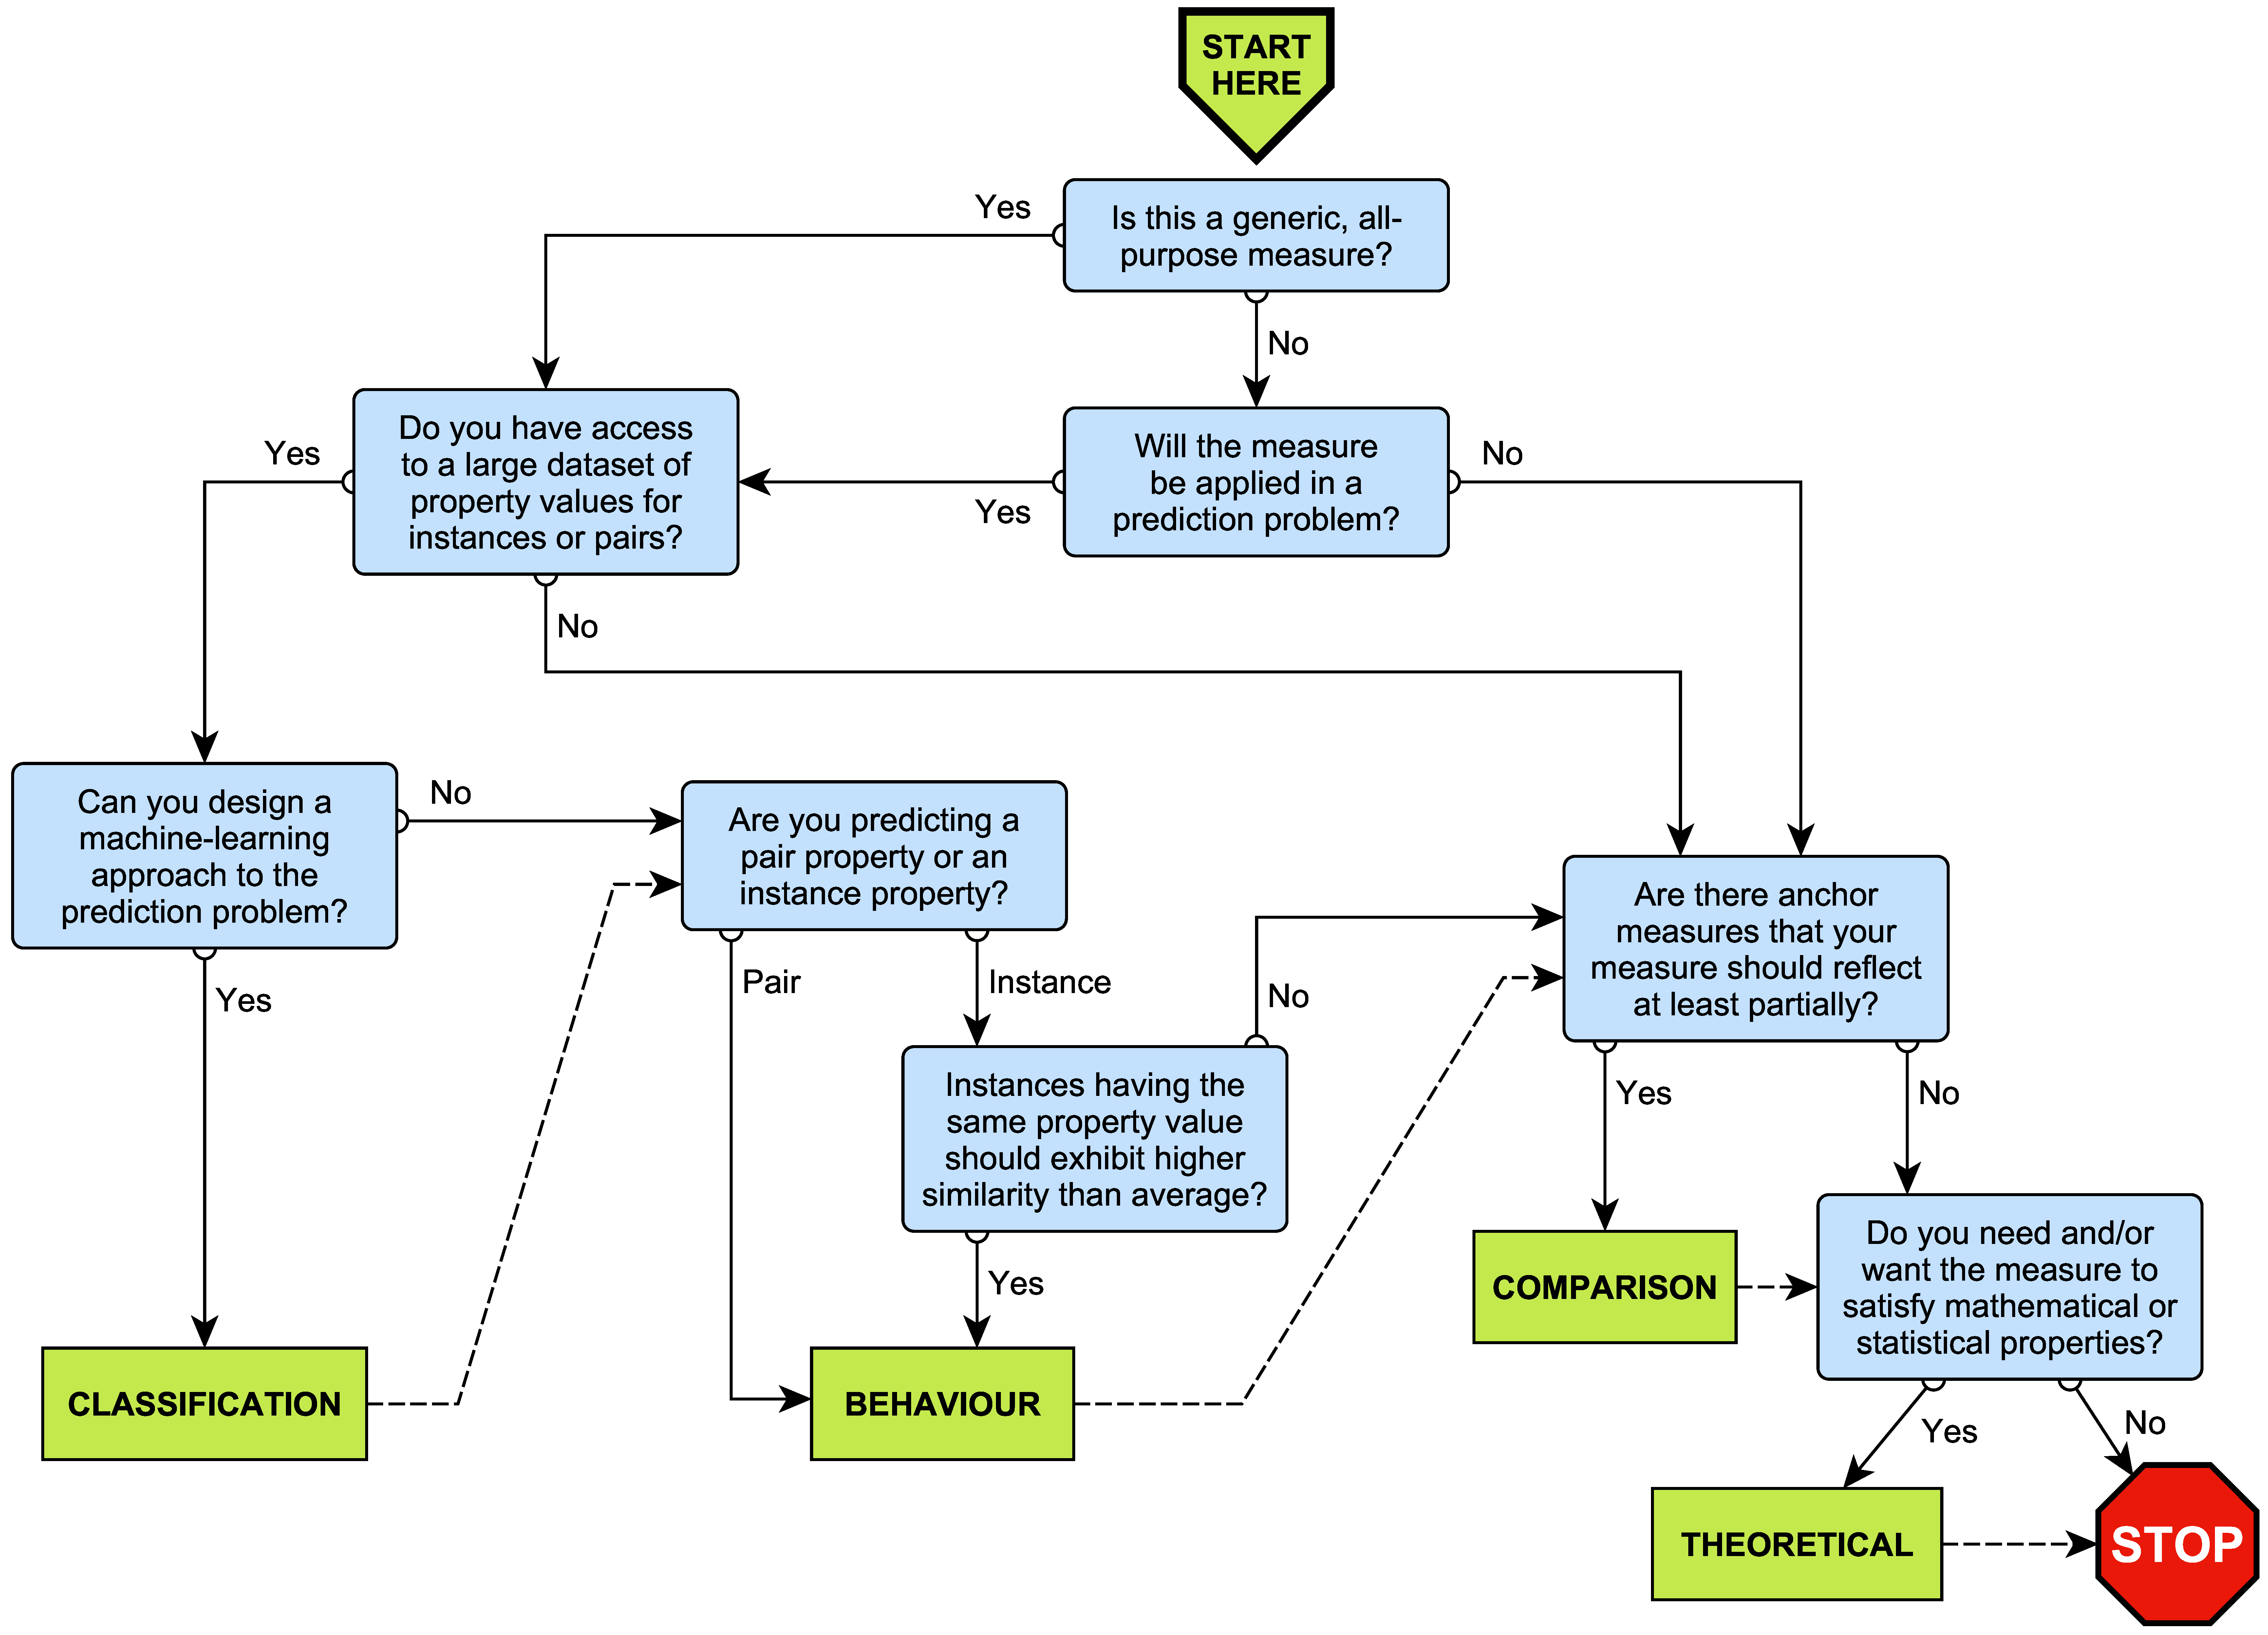
\includegraphics[width=0.8\textheight]{images/diagram.pdf}
    \end{turn}
    \caption[Pipeline to assist semantic similarity developers in the validation step]{Specific classes should be selected according to the data that the developers have access to, and to the overall goal of the measure. Questions the developers must answer are in blue rounded rectangles; strategy types are in straight green rectangles. The diagram anticipates the possibility of simultaneous validation strategies by drawing arrows from the resulting strategy types to additional questions (dashed arrows).}
    \label{fig:diagram}
\end{figure}

\chapter{Towards OWL-aware similarity} \label{chap:enhancements}

The biomedical informatics community is actively committed to the adoption of formal-logic knowledge representation languages, such as the Web Ontology Language (OWL), and the use of reference ontologies to annotate biomedical resources (\cf \appref{app:ontologies}). This adoption has resulted in the increase of
\begin{paralist}
    \item the amount of knowledge represented in ontologies, and
    \item the quality of these representations in respect to the reality.
\end{paralist}

As has been argued by \citet{Couto2013}, there are some benefits to considering exploiting formal axioms in the calculation of semantic similarity. In this chapter, I report the enhancements that I achieved in the pursuit of semantic similarity measures that can maximise the use of these axioms. I first report on a measure that can use disjointness axioms and then on another that can use existential quantifications.


\section{Disjointness axioms in semantic similarity} \label{sec:enhancements/disjointness}

\begin{note-paper}
    This section is adapted from a paper produced in collaboration with Janna Hastings from the European Bioinformatics Institute, published in Oxford Bioinformatics~\citep{Ferreira2013}.
\end{note-paper}


\subsection{The idea}

Disjointness axioms are one example of formal constructions in OWL ontologies that are gaining momentum in the biomedical informatics community. For example, the Chemical Entities of Biological Interest (\ontology{CHEBI}) ontology now includes this type of axioms~\citep{Hastings2013}. To explore this new type of information, I devised an algorithm that can be \emph{plugged} into some semantic similarity measures to take into account disjointness information.

A disjointness axiom declared for a pair of concepts express the constraint that an instance of one of them cannot also be an instance of the other. This constraint logically implies that the two concepts cannot have common subclasses. Should such shared subclasses be detected by a reasoner, the reasoner will flag the ontology as \emph{inconsistent}~\citep{Sattler2013}, which can be used by ontology developers to prevent errors in ontology development. For example, in \ontology{CHEBI}, this technique has been used to detect that a specific ion (a type of charged molecule) was misclassified as a group (a strict part of a molecule)~\citep{Hastings2012}.

\begin{figure}
    \centering
    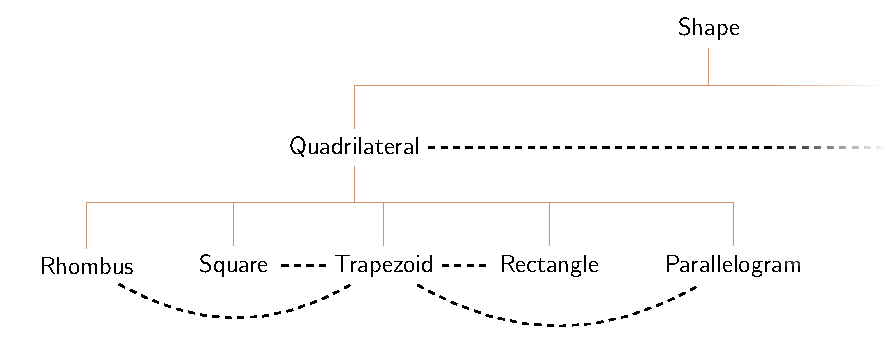
\includegraphics[width=\textwidth]{images/shape-ontology.pdf}
    \caption[A snippet of a hypothetical Shape Ontology]{In this snippet, I use the term \term{Parallelogram} as ``a quadrilateral with two pairs of parallel sides'' and \term{Trapezoid} to mean ``a quadrilateral with two parallel sides and two obtuse angles''. Solid lines represent class-subclass relationships, dashed lines represent disjointness axioms. Note that a proper shape ontology would classify \term{Square} as a subclass of \term{Rectangle}, \term{Rhombus} and \term{Parallelogram}, and \term{Rhombus} as equivalent to \term{Parallelogram}. For the sake of the argument being exposed, however, assume that such information is yet unknown by the ontology creators.}
    \label{fig:shape}
\end{figure}

\figref{fig:shape} illustrates this situation: this ontology snippet asserts that no instance of \term{Rectangle} can simultaneously be an instance of \term{Trapezoid}. However, given the open-world assumption that underlies OWL ontologies (see \secref{sec:concepts/ontologies}), there can be instances of \term{Rectangle} that are also instances of \term{Parallelogram} (in fact, it is a consequence of the relevant geometric definitions that squares are both rectangles and parallelograms). For this reason, the similarity between \term{Rectangle} and \term{Parallelogram} should intuitively be higher than the similarity between \term{Rectangle} and \term{Trapezoid}. Using $\sigma$ to represent the function that returns the similarity between two concepts, this hypothesis can be mathematically stated with \eqref{eq:motivation}:
\begin{equation}
    \sigma(\term{Rectangle}, \term{Parallelogram}) >
    \sigma(\term{Rectangle}, \term{Trapezoid}).
    \label{eq:motivation}
\end{equation}


\subsection{The proposed measure} \label{sub:disjointness/measure}

As has been discussed in \secref{sec:sota/node}, there has been an effort to design measures that compute the shared information content between two concepts: while shared information content between concepts $x$ and~$y$ has been assumed to be well estimated by the maximal information content of the concepts that subsume both $x$ and~$y$, \citet{Couto2011} suggest DiShIn, a shared information content measure that builds upon existing measures (such as the ones in \eqref{eq:resnik-ssm,eq:lin}) and which behaves as a \emph{plug-in} to such measures. In its particular case, DiShIn explores \emph{multiple parentage} in order to ensure that all shared information across multiple ancestors is taken into account.

Likewise, instead of developing a new semantic similarity measure to deal with disjointness axioms, I proposed a \emph{plug-in} to be used on top of existing measures of shared information content. My \emph{plug-in} refines the estimation of shared information between two concepts by incorporating the disjointness axioms asserted in the ontology. In here, I denote the disjointness-aware measure of shared information content between concepts $x$ and~$y$ as $\ICsdis(x,y)$, which is calculated based on an existing measure of shared information content,~$\ICs(x,y)$.

Given the example presented in \figref{fig:shape} and the inequality of \eqref{eq:motivation}, it would be desirable for the measure of shared information content to decrease for concepts that are known to be disjoint, formalising the intuition that disjoint concepts are less similar because they cannot share subclasses. Furthermore, to respect the open-world assumption, the measure should stay unchanged when two concepts are \emph{not known} to be disjoint.

With these constraints in mind, I proposed the following measure of shared information content:
\begin{equation}
    \ICsdis(x,y) = \ICs(x,y) - k(x,y)
    \label{eq:new-disj}
\end{equation}
where $\ICs(x,y)$~is any measure of shared information content between $x$ and~$y$, $k(x, y) > 0$ if $x$ and~$y$ are disjoint and $k(x, y) = 0$ otherwise.

\begin{figure}
    \centering
    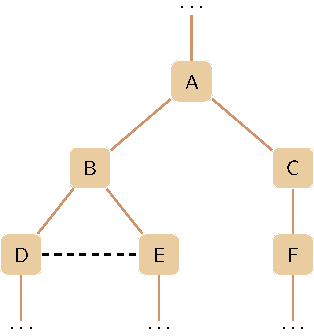
\includegraphics[width=0.35\textwidth]{images/toy-disjoints.pdf}
    \caption[Example ontology with disjointness axioms]{This illustrates a toy ontology that shows some concepts in a class-subclass hierarchy (represented with solid lines) as well as a disjointness axiom asserted between two concepts (dashed lines).}
    \label{fig:toy}
\end{figure}

Two points were crucial in the development of this measure. First, note that, as is, this equation presents a \emph{discontinuity}. In the hypothetical ontology of \figref{fig:toy}, this measure implies
\begin{equation}
    \ICsdis(\term D, \term E) < \IC(\term B),
\end{equation}
which, depending on the value $k(\term D, \term E)$, could lead to
\begin{equation}
    \ICsdis(\term D, \term E) < \IC(\term A) = \ICsdis(\term D, \term F).
\end{equation}
However, this should not be possible, since \term D and \term E share more information than \term D and~\term F. Therefore, $k$ must be bounded according to the $\IC$ of the most informative ancestor of the $\MICA$, which, in this case, results in
\begin{equation}
    k(\term D, \term E) \leq \IC(\term B) - \IC(\term A).
\end{equation}

\begin{figure}
    \centering
    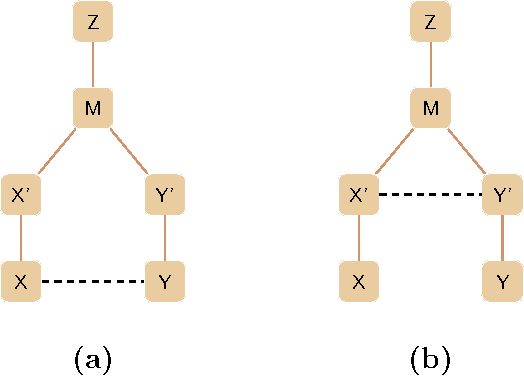
\includegraphics[width=0.594\textwidth]{images/strength.pdf}
    \caption[The potential for implicit common superclasses between two concepts]{In both cases, $\MICA(\term X, \term Y) = \term M$, and the most informative ancestor of \term M is \term Z. The difference is in the location of the disjointness axiom. In situation A, there is a higher likelihood of implicit common ancestors (ICA) between \term X and~\term Y, because the axiom of disjointness is further down from their common ancestry.}
    \label{fig:strength}
\end{figure}

The second major decision in the development of this measure is related to an operational notion. In fact, I have not yet defined how to compute~$k(x,y)$. I propose an algorithm based on the notion of potential for \emph{implicit common superclasses} (ICS), which measures the likelihood that two concepts share non-asserted superclasses. Consider the ontology snippets in \figref{fig:strength}. In situation~A, given the open-world assumption, there is a small chance that \term Y turns out to be a subclass of~$\term{X'}$, while in situation~B that cannot happen, since \term Y is inferred to be disjoint with~$\term X'$ (the disjointness axiom is higher up in the hierarchy). This suggests that there is a higher potential for ICS between the concepts \term X and~\term Y in situation~A.

I model the \emph{unlikelihood} of ICS as~$f(x, y)$, a function that returns higher values for situations with lower potential for ICS:
\begin{equation}
    f(x, y) =
    \max\left\{
        \frac{1}{p(a,b)} \,\Big|\, a\in\anc(x) \wedge b\in\anc(y) \wedge J(a,b)
    \right\}\cup\{0\}
\label{eq:strength}
\end{equation}
where $\anc(c)$~is the set of superclasses of~$c$ (including~$c$), $J(a, b)$~is true when $a$ and~$b$ are disjoint (either by assertion or inference) and false otherwise, and $p(a, b)$~is the edge length of the shortest path from $a$ to~$b$, taking into account only class-subclass relationships, not the disjointness arcs (only the solid edges in the figures, not the dashed ones).

Using the example ontologies in \figref{fig:strength}, we can illustrate this definition by calculating~$f(\term X, \term Y)$. In A, $J(a,b)$~is true only for $(a,b)=(\term X, \term Y)$; the shortest path from \term X to~\term Y is $\term X \rightarrow \term{X'} \rightarrow \term M \rightarrow \term{Y'} \rightarrow \term Y$, which has length~$4$. Therefore,
\begin{equation}
    f(\term X, \term Y)=\max\left\{\frac14,0\right\}=\frac14.
\end{equation}

In B, $J(a,b)$~is true for $(a,b)\in\{(\term X, \term Y), (\term X, \term{Y'}), (\term{X'}, \term Y), (\term{X'}, \term{Y'})\}$. These correspond to paths of length $4$, $3$, $3$ and~$2$, respectively, leading to
\begin{equation}
    f(\term X, \term Y) = \max\left\{\frac14, \frac13, \frac12, 0\right\}=\frac12.
\end{equation}

Additionally, in situation A, $f(\term{X'}, \term{Y'}) = 0$, since the two concepts are not disjoint and as such $J(a,b)$~is always false.

The general procedure to calculate $\ICsdis(x,y)$ is, therefore:
\begin{enumerate}
    \item Determine $M = \MICA(x,y)$
    \item Determine $Z = \argmax_c \{\IC(c)\,|\,c\in\anc(M)\}$, \ie the most informative ancestor of~$M$;
    \item Calculate $f(x, y)$, as described in \eqref{eq:strength};
    \item Calculate $k(x,y) = f(x,y)\cdot(\IC(M) - \IC(Z))$;
    \item Calculate $\ICsdis(x,y)=\ICs(x,y)-k(x,y)$.
\end{enumerate}

With this procedure, the new shared information content is estimated as a weighted average between $\IC(M)$ and~$\IC(Z)$, where a low potential for ICS leads to a shared information content close to~$\IC(Z)$ and a higher potential for ICS leads to a shared information content close to~$\IC(M)$. This means that the shared information content decreases by a larger amount when there is a smaller potential for implicit common superclasses. Note that if the two concepts are not disjoint, $k(x,y)=0$ and $\ICsdis=\ICs$, which satisfies the open-world assumption mentioned previously.


\subsection{Validation}

According to the hierarchy presented in \chpref{chap:validation}, I classify the validation approach followed in this work as a ``Comparison with an anchor measure''. For this purpose, I calculated structural similarity between \ontology{CHEBI} concepts (details can be found on the paper), and semantic similarity using the algorithm described above, and measured the Pearson's correlation coefficient between the two measures.

The proposed measure was validated in three steps, by measuring the increase in coefficient
\begin{paralist}
    \item in the presence \vs absence of disjointness axioms,
    \item with increasing fractions of the total number of disjointness axioms, and
    \item in several random datasets.
\end{paralist}

For a fully detailed discussion of these three steps, I refer the reader to the published paper. Here I summarise the main results.

\point{Increase in correlation coefficient} I applied the new measure of shared information content to a subset of \ontology{CHEBI}, including some disjointness axioms~\citep{Hastings2012,Hastings2013}. Since it consists of a \emph{plug-in} and relies on a previously defined measure of shared information content, I used, in this assessment, the classical notion of shared information content proposed by~\citet{Resnik1995}:
\begin{equation}
    \ICs(x,y) = \IC(\MICA(x,y))
\end{equation}
where information content was calculated using \eqref{eq:seco}.

Given the sparsity of disjointness axioms relative to the size of \ontology{CHEBI}, random pairs of concepts would rarely touch any disjointness information and it would be difficult to detect the difference resulting from these axioms. As such, the concepts in the dataset were chosen so that a significant part of them had disjointness information. Additionally, given the need to calculate structural similarity, the concepts in the dataset were also selected in order to ensure that structural similarity was possible. While these two constraints slightly bias the generated dataset, I believe that the bias did not result in a dataset too different from reality: in fact, although the amount of disjointness axioms already added to \ontology{CHEBI} is not high, true disjointness exists for most pairs of concepts.

Structural similarity was calculated using PubChem's fingerprint method~\citep{Bolton2008}. Structural similarity between \ontology{CHEBI} concepts that do not represent actual molecules but rather chemical groups (\eg there is not a single chemical structure for \term{Hexose} but rather a collection of them) was achieved by comparing the collection of structures.

For the dataset created above, I compared all compounds with all
the other compounds using three measures: structural similarity, classical $\ICs$ and~$\ICsdis$. I used Wolfe's t-Test~\citep{Wolfe1976,Rosner2010} to determine the statistical significance of the increase in the correlation coefficient between the pair~$(\textrm{structural}, \ICs)$ and the pair~$(\textrm{structural}, \ICsdis)$.

The Pearson's correlation coefficient between the structural measure and~$\ICs$ is~$0.69883$, and after taking the disjointness axioms into account, the correlation between structural similarity and~$\ICsdis$ becomes~$0.71571$. This represents an increase of~$0.01688$. Despite the small absolute increase, this value is statistically significant, with a~\emph{p}-value of~$4.5 \times 10^{-8}$. The small increase of the correlation can be attributed to at least three
factors:
\begin{itemize}
    \item As the annotation of disjointness is still incomplete in \ontology{CHEBI}, we have access to only a small subset of all the \emph{real} disjointness axioms that can be expressed in \ontology{CHEBI}, which means that the shared information content changes only for a fraction of all the concept pairs ($39\%$ of the pairs in the dataset). I expect that, as the number of disjointness axioms added to \ontology{CHEBI} increases, both this fraction and the difference between correlation coefficients will increase.
    \item While highly correlated, structural similarity and semantic similarity measures are inherently different, and as such there is a maximum bound on the actual correlation that can be expected between the two (\cf \secref{sub:hierarchy/comparison}).
    \item Disjointness is only one of the logical axiom types that are used to express concept definitions in an OWL ontology. In fact, \ontology{CHEBI} contains a number of other properties that are also used to capture the meaning of its concepts, \eg the property \prop{has-tautomer}, which connects together closely structurally related chemicals, and \prop{has-role}, which connects a chemical concept to its biological activity.
\end{itemize}


\point{Effect of the number of axioms} The second assessment step measured the effect of the number of disjointness axioms on the correlation coefficient. I partitioned the $199$~disjoitness axioms into $10$~sets: the first contained $20$~random axioms, the second contained these plus another $20$~random axioms, \etc., with the final one containing the $199$~axioms (see \figref{fig:partitions}). For each set, I calculated $\ICsdis$ on the previous dataset and plotted a graph showing the increase in correlation \vs the number of axioms. To remove any bias that resulted from the random method used to partition the axioms, I repeated this process $20$~times.

\begin{figure}
    \centering
    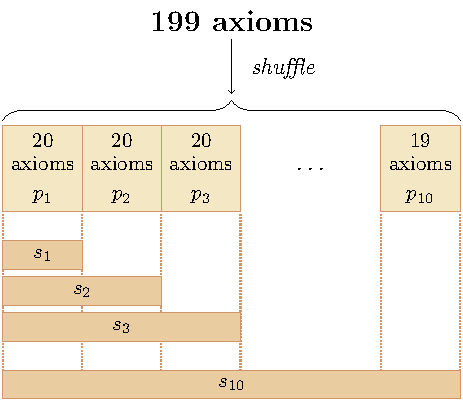
\includegraphics[width=0.6\textwidth]{images/partition.pdf}
    \caption[Partitioning the set of disjointness axioms]{The process used to assess the effect of the number of axioms on the correlation coefficient between structural and semantic similarity. The axioms are randomly partitioned into clusters $p_1$ to~$p_{10}$. Consecutively, each of these clusters is joined with the previous ones to create the sets $s_i = \bigcup_{j=1}^i p_j$, which are then used to compute the increase in correlation coefficient.}
    \label{fig:partitions}
\end{figure}

This validation step has the objective of simulating the development of \ontology{CHEBI} ontology with respect to the number of disjointness axioms. For each of the $20$~repetitions, I studied the difference between the correlation coefficients as the number of disjointness axioms increases, and plotted a graph with this information.

The graphs in \figref{fig:evolution} show the result of some of these repetitions. These graphs illustrate that not all disjointness axioms are important for a given dataset. In fact, only for some of the sets of axioms is the correlation coefficient significantly affected, which suggests that those sets contained the axioms that change the logical meaning behind the concepts in the dataset. The graphs present an obvious trend (see \figref{fig:evolution-trend} for an average of the graphs of all the $20$~repetitions) that indicates an increase of the correlation, which, again, indicates that the disjointness axioms improve the correctness of semantic similarity.

\begin{figure}
    \centering
    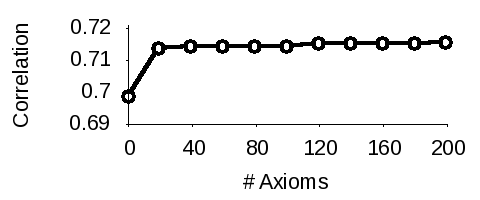
\includegraphics[width=0.4\textwidth]{images/plot18.png}
    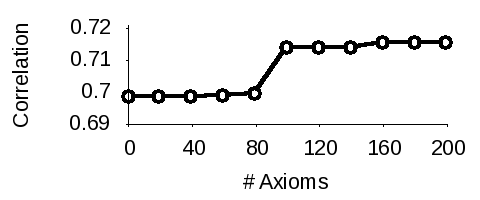
\includegraphics[width=0.4\textwidth]{images/plot17.png}
    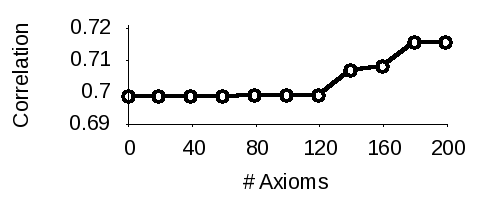
\includegraphics[width=0.4\textwidth]{images/plot3.png}
    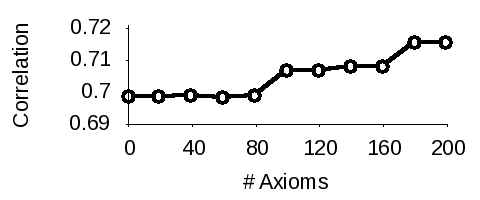
\includegraphics[width=0.4\textwidth]{images/plot1.png}
    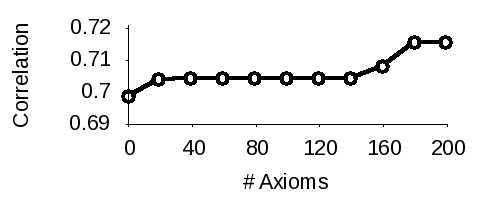
\includegraphics[width=0.4\textwidth]{images/plot10.png}
    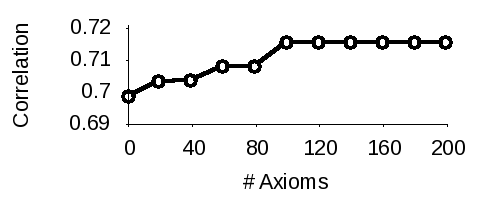
\includegraphics[width=0.4\textwidth]{images/plot8.png}
    \caption[The effect of increasing number of disjointness axioms]{These graphs illustrate the increase in correlation coefficient that results from increasing the number of disjointness axioms. In each graph, the abscissa is the number of axioms used by the semantic similarity measure and the ordinate is the correlation coefficient. The correlation coefficient for $0$~axioms is always equal to the correlation measured with the classical~$\ICs$, which is~$0.69883$; the correlation coefficient for the maximum number of axioms corresponds to the value~$0.71571$, presented in the first validation step. These graphs are representative of the behaviour obtained in all the $20$~repetitions.}
    \label{fig:evolution}
\end{figure}

\begin{figure}[p]
    \centering
    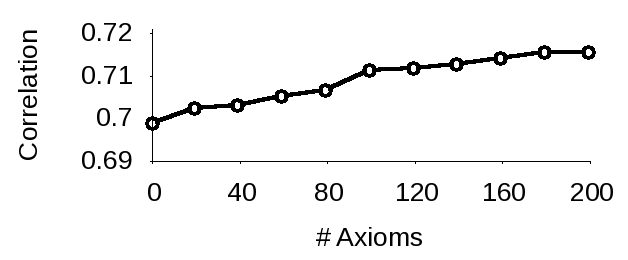
\includegraphics[width=0.6\textwidth]{images/trend.png}
    \caption[The trend corresponding to all the repetitions]{This graph shows the average of all the graphs produced in the $20$~repetitions. Although these values do not have any statistical significance in themselves, they clearly show the trend that the more disjointness axioms are considered, the better is the correlation between structural and semantic similarity.}
    \label{fig:evolution-trend}
\end{figure}


\point{Effect on other datasets:} As the third assessment step, I studied the increase in correlation coefficient on other datasets, since the dataset created for the first step resulted from a random selection process. Following the same selection process, I created $550$~more datasets and compared the correlation coefficient as previously explained.

The graph of \figref{fig:histogram} shows an histogram that represents the difference in the Pearson's correlation coefficient for all these datasets. As is visible in that graph and in \tabref{tab:histogram}, the vast majority of the datasets are associated with an increase in the correlation coefficient. In fact, the effect of considering the disjointness axioms for the semantic similarity only impacts negatively $6.2\%$ of the datasets. We observed a mean correlation increase of~$0.0149$, with a standard deviation for that value of~$0.0130$. Furthermore, in $72.5\%~$of the datasets, the increase in correlation is significant at a confidence value of $0.05$.

\begin{figure}[p]
    \centering
    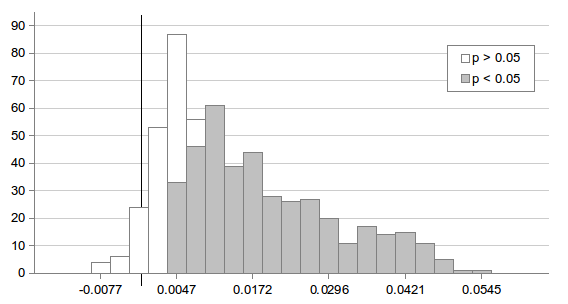
\includegraphics[width=0.7\textwidth]{images/histogram.png}
    \caption[Distribution of the difference in correlation coefficient for random datasets]{The majority of the cases show a positive difference. I used Wolfe's t-Test to calculate the \emph{p}-value associated with the hypothesis that the increase was due to random chance, and marked with a darker shade the amount of datasets for which p-value${}<0.05$. The vertical line shows the zero of the axis, \ie where the two correlation coefficients are the same.}
    \label{fig:histogram}
\end{figure}

\begin{table}[p]
    \centering
    \small
    \caption[Statistics related to the histogram of \figref{fig:histogram}]{The last column shows the frequency relative to all the datasets created.}
    \begin{tabular}{lrr}
    \toprule
        & \bfseries \# datasets & \bfseries \% datasets \\
    \midrule
    Increase in correlation & 516 &  93.8\% \\
    p-value${}<0.05$        & 399 &  72.5\% \\
    \bottomrule
    \end{tabular}
    \label{tab:histogram}
\end{table}


\subsection{Limitations, future work and other conclusions}

This measure has some limitations:
\begin{enumerate}
    \item The formula of~$\ICsdis$ is not robust against ontology development. Sometimes, the addition of a concept to the ontology during development can considerably change the value of shared information content between two concepts (\cf \secref{sub:hierarchy/theoretical}, where I mention this problem in the context of semantic similarity validation). This issue is mitigated by the fact that the such additions are not common in biomedical ontologies (full details in the paper).
    \item The potential for implicit common superclasses is measured using an edge distance, which is a fragile measure in biomedical ontologies~\citep{Pesquita2009} (see \secref{sec:sota/edge}). It may be possible to explore the semantics of the edges themselves in order to overcome this issue.
    \item The measure of information content influences the results obtained with~$\ICsdis$. In this case, IC was calculated with an intrinsic measure of information content; it would be informative to see the effect of changing the IC measure to an extrinsic one.
\end{enumerate}

This validation shows that considering disjointness axioms improves the shared information content measure, with statistical significance. This new approach is able to successfully explore more than just the class-subclass hierarchy of an ontology, relying on a partial subset of the description logic axioms that are included in the ontology to refine the comparison algorithm. To the best of my knowledge, this represents the first attempt to explicitly use description logic expressivity in semantic similarity in the biomedical domain. I demonstrated this hypothesis using a rather naïve approach. More sophisticated approaches include the exploration of the semantics of edges, other types of information content based on external corpus, \etc.

\section{Semantic relatedness measure} \label{sec:enhancements/relatedness}

\begin{note-paper}
    This section is adapted from a papers accepted for oral presentation at the International Conference on Biomedical Ontology~2011 and published in the corresponding proceedings~\citep{Ferreira2011}.
\end{note-paper}

\subsection{The idea}

According to the definition provided in \secref{sec:concepts/semantic-similarity}, semantic similarity uses exclusively the hypernymy relationship of an ontology: the class-subclass hierarchy. In this sense, \term{Heart} and \term{Blood} are not similar at all. However, in some contexts, hypernymy is not enough to detect that two concepts are related to one another. Anatomy, specifically when used to detect similarity between diseases, is one of these contexts. For example, a heart disease can have implications in blood pressure, and thus a disease annotated with the concept \term{Heart} is somewhat related to one annotated with the concept \term{Blood}.

\begin{figure}[!b]
    \centering
    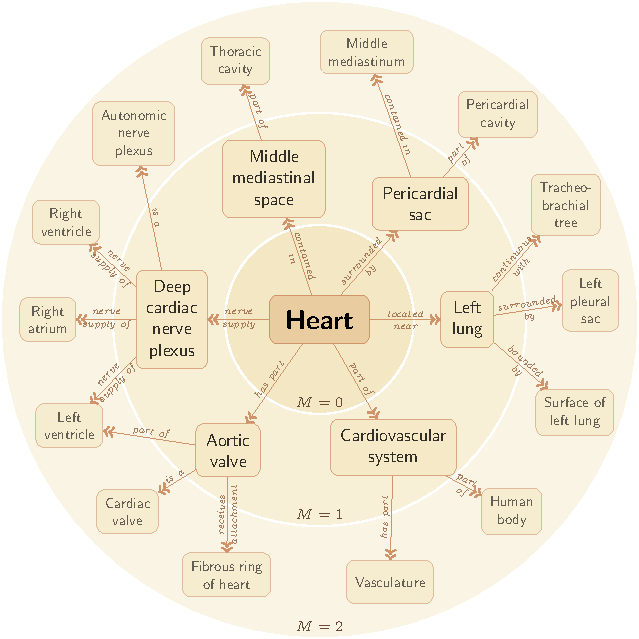
\includegraphics{images/heart-neighbourhood.pdf}
    \caption[The semantic neighbourhood of the concept \term{Heart}]{This picture illustrates the semantic neighbourhood of \term{Heart}, with a radius~$M=2$. As depicted, \term{Aortic valve} is part of the first layer since it directly links to \term{Heart}, while \term{Cardiac valve} is part of the second layer. Notice that some neighbours can be connected to the centre by more than one distinct path (\eg \term{Left ventricle}). The \emph{radius} can be increased, resulting in a larger neighbourhood. Given the proposed weighting mechanism (see \eqref{eq:weight}), the closer the concepts are to the centre, the higher is their contribution to the semantic neighbourhood of \term{Heart}.}
    \label{fig:heart-neighbourhood}
\end{figure}

I developed a measure that compares two anatomical entities based on their ``semantic neighbourhood'', an idea that was based on the mental processes that take place in the human mind when comparing concepts~\citep{Quillian1968,Collins1975,Tversky1977} (see \secref{sec:sota/art}). The semantic neighbourhood of a concept is a graph, where each node is a concept and an edge between two nodes is drawn if the two concepts are related in the ontology by means of an existential quantification axiom (see \secref{sec:concepts/owl}). Consider \figref{fig:heart-neighbourhood}, which shows a snippet of the semantic neighbourhood of \term{Heart} as defined in the Foundational Model of Anatomy (\ontology{FMA}). In here, we can see that \term{Heart} is related to \term{Aortic valve} by the property \prop{has-part}. Many other concepts are related to \term{Heart}. The neighbourhood is extended by allowing the neighbours of the neighbours to participate in it as well, recursively. I call the maximal distance between the centre concept and its neighbours the ``radius'' of the neighbourhood, represented by~$M$ and measured in number of edges in the graph. Notice, then, that we can compute the neighbourhood up to any particular radius, and that a wider neighbourhood can convey more information about a particular concept than a narrower one. Using this notion, comparing two concepts is a matter of comparing the two neighbourhoods, and this was exactly what I proposed~\citep{Ferreira2011}.

Notice that, again, this corresponds to extending the notion of semantic similarity to more logical constructions, in this case the existential quantification. In formal logic, we say that, for each \term{Heart} there is a relationship of type \prop{part-of} between that \term{Heart} and some \term{Aortic valve}:
\begin{axiom}
    \existential{Heart}{has-part}{Aortic valve}
\end{axiom}
Understanding this notation is not essential to appreciate the contributions presented in this document (details and further exploration of description logic symbols can be found, \eg in works by \citet{Nardi2003} and \citet{Baader2005}). Simply take into account that this means ``Each heart has an aortic valve'' (we will encounter this exact notation again in the next chapters).

\ontology{FMA} is one of the best test cases to assess the behaviour of this measure, as it is rich in existential quantifications. In fact, it contains $67$~distinct properties (\eg \prop{part-of}, \prop{surrounded-by}, \prop{continuous-with}, \etc.), which are used in more than $200{,}000$~axioms.

Finally, the same figure can be used to show the concepts of ``weight''. The path from \term{Heart} to \term{Aortic valve} is smaller than the one from \term{Heart} to \term{Vasculature}, which means that \term{Aortic valve} is somehow more related to \term{Heart} than \term{Vasculature}. I use the notion of ``weight'' to measure this relative relatedness within a semantic neighbourhood.


\subsection{The proposed measure}

Mathematically, the relatedness between two concepts $x$ and~$y$, is defined as:
\begin{equation}
\ferreira(x,y) = \frac
    {\sum_{i\in N_M(x) \cap N_M(y)} \, \weight ix \otimes \weight iy}
    {\sum_{i\in N_M(x) \cup N_M(y)} \, \weight ix \oplus  \weight iy}
    \label{eq:ferreira}
\end{equation}
where $N_M(c)$~is the semantic neighbourhood of a concept~$c$ calculated to a maximal radius~$M$, and $\weight ic$~is a weighting function that gives more relevance to the concepts that are closer to~$c$ and less relevance to concepts further away.

This formula is relatively complex in syntax, and uses non-standard mathematical operations, and as such needs to be explained bit by bit. In essence, it is a ratio between what is common in the semantic neighbourhoods of $x$ and~$y$, and the total amount of concepts in the two neighbourhoods. This idea is not far from what is used in $\sim[UI]$ and~$\sim[GIC]$ (see \eqref{eq:simui,eq:simgic}). Unlike those measures, each concept has now two weights, one for each neighbourhood. To deal with this multiplicity of weights, I used the binary operators of T-norm and T-conorm, represented mathematically by the symbols $\otimes$ and~$\oplus$, respectively, which can be applied to two values between $0$ and~$1$. There are several T-norms and T-conorms that could be applied. Mathematically I am interested in the following properties:
\begin{align*}
    0          & \le i \otimes j \le \min(i, j) \\
    \max(i, j) & \le i \oplus j \le 1.
\end{align*}
I chose $x \otimes y = x y$ and $x \oplus y = x + y - x y$~\citep{Klement2004}.

Consider two semantic neighbourhoods, one for concept~\term A and another for concept \term B. We want the concepts that belong to both neighbourhoods to increase the overall measure in a way that is related to how important these two concepts are in the two neighbourhoods. For a concept~$c$ that belongs to both neighbourhoods, let $w_A=\weight cA$ and~$w_B=\weight cB$ be the weights of this concept with respect to each of the two neighbourhoods. Consider the following fraction:
\begin{equation}
    \frac{w_A \otimes w_B}{w_A \oplus w_B} =
    \frac{w_A \times w_B}{w_A + w_B - w_A \times w_B}.
\end{equation}
If $c$~is highly relevant in both neighbourhoods (\eg $w_A=0.8$ and~$w_B=0.9$), both the numerator and the denominator of this fraction have a high value~($\frac{0.72}{0.98}$) and, as such, we observe an increase in the overall $\ferreira$ (\eqref{eq:ferreira}). If both have a low relevance (\eg $w_A=0.1$ and~$w_B=0.2$), the numerator will be a low value and the denominator will be a medium-range value~($\frac{0.02}{0.28}$), which contribute to a mild decrease in the overall measure. But if the concept has high relevance in one neighbourhood and low relevance in the other (\eg $w_A=0.2$ and~$w_B=0.9$), the numerator will be low and the denominator will be high~($\frac{0.18}{0.92}$), which will contribute to a large decrease in the overall measure.

By default, I propose that the weight of a concept with respect to a neighbourhood is computed based on the path that connects that concept to the centre of the neighbourhood. Let~$p_c$ be a path connecting concept~$c$ to the centre of the neighbourhood. This path is composed of a sequence of properties. For example, in \figref{fig:heart-neighbourhood}, the path from \term{Heart} to \term{Cardiac valve} is ``\prop{has-part}${}\rightarrow{}$\prop{is-a}''. The weight associated to a certain path is the product of the relevance of each of the properties in the path. If more than one path can be traversed from the centre to the concept, then I take the maximum relevance associated with these paths. Formally, let~$r(i)$ be the relevance of the property~$i$: then
\begin{equation}
    \weight cA=\max_{p_c}\prod_{i \in p_c} \mathrm{r}(i).
    \label{eq:weight}
\end{equation}
Finally, the relevance of each property must be predetermined before running this algorithm. I originally proposed using~$0.7$ as the default relevance, on the basis that it produced the best results from a selection of possible default values ($0.6$, $0.7$ and~$0.8$). With the passing of time, I came to realise that we could assign each property a relevance that is based on its own information content. Recall the formula used to calculate the information content of a concept based on the ontology alone, proposed by \citet{Seco2004}~(\eqref{eq:seco}). Reusing this formula here, and taking the frequency of a property to be the number of existential quantification axioms in the ontology that use it, we can also define the information content of properties:
\begin{equation}
    \IC(i) = 1 - \frac{\log f(i)}{\log N_e}
\end{equation}
where $f(i)$~is the number of existential axioms that use property~$i$ and $N_e$~is the number of existential axioms in the ontology.

Furthermore, notice that this measure can both calculate the similarity between concepts and the similarity between annotated entities. In fact, the construction of a semantic neighbourhood can either start on a single concept or on a set of concepts, making this a group-wise relatedness measure.


\subsection{Validation}

The validation strategy followed in this work can be classified as a ``Classification prediction''. I based this validation on the assumption that anatomical entities implicated in the same disease should be more related than a random pair of anatomical entities. I first created a map between diseases and \ontology{FMA} concepts. To do that, I used the Human Phenotype Ontology (\ontology{HPO}), an ontology that represents abnormalities in human anatomy (such as \term{Abnormality of the eye} or \term{Prostate cancer}). On the one hand, this ontology is used by its creators to annotate diseases from several disease databases, and associates $6882$ \ontology{HPO}~concepts with $8013$~diseases, with an average and median of $15$ and~$9$ \ontology{HPO}~concepts for each disease, respectively. On the other hand, the ontology itself provides semi-formal descriptions of its concepts, with references to \ontology{FMA} concepts. For example, \term{Microtia} is described as:
\begin{quote}
    Underdevelopment of the external ear (\ontology{FMA}:52781).
\end{quote}
By leveraging on the annotations mentioned above and these \ontology{FMA} references, it is possible to create a dataset of \ontology{FMA}-annotated diseases (see \figref{fig:disease2fma}). This dataset can then be used to find pairs of anatomical concept that are implicated in the same disease, which correspond to the positive dataset for this validation. The negative dataset was generated randomly.

\begin{figure}
    \centering
    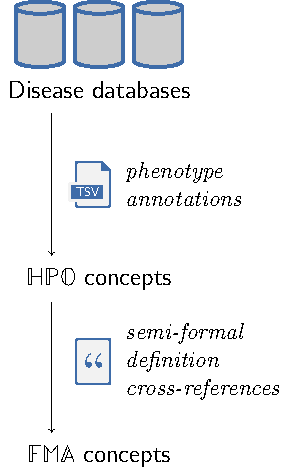
\includegraphics{images/disease2fma.pdf}
    \caption[Workflow to find \ontology{FMA} annotations for some diseases]{The first step is to find the annotations from diseases to \ontology{HPO} concepts, which are provided as \texttt{TSV} files in the \ontology{HPO} website; the second step is to leverage on the cross-references that exist in the textual definitions of the \ontology{HPO} concepts to convert them into \ontology{FMA} concepts. This allows one disease to be associated (\ie annotated) with a set of \ontology{FMA} concepts.}
    \label{fig:disease2fma}
\end{figure}

The positive and negative datasets were then used to perform Receiving Operating Characteristic (ROC) analysis~\citep{Fawcett2006}. This is a common step in classification approaches, summarised as follows:
\begin{enumerate}
    \item Select a threshold~$t$ and create a binary classifier that classifies as positive all the pairs that have $\ferreira>t$ and as negative the other. For each~$t$, we can determine the true positive rate (TPR \mdash fraction of the related concepts correctly classified as related) and false positive rate (FPR \mdash fraction of the unrelated concepts incorrectly classified as related).
    \item The highest threshold results in a TPR of~$0$ and a FPR of~$0$ (all pairs are classified as negative); likewise, the lowest possible threshold results in a TPR of~$1$ and a FPR of~$1$ (all pairs are classified as positive).
    \item Plot the curve defined by the points $(\textrm{FPR}, \textrm{TPR})$ when the threshold varies from the maximum to the minimum. This is known as the ROC curve. The closer the graph approaches the point~$(0, 1)$ (which represents the ideal case where all the positive pairs have a higher relatedness measure than all negative pairs), the better is the measure of relatedness.
    \item \citet{Fawcett2004} proposes a way to repeat this experiment a number of times and to produce an average ROC curve from them (see Algorithm~5 of that paper), which I followed by repeating these steps $10$~times, each time with a different randomly generated negative dataset.
\end{enumerate}

The ROC curves obtained with this method are presented in \figref{fig:roc}. For comparison purposes, I applied the proposed $\ferreira$~measure, calculated for $M=3$ and~$M=4$, and I also applied~$\sim[GIC]$ to the dataset to study how the behaviour of a similarity measure contrasts with the behaviour of a relatedness measure.

\begin{figure}
    \centering
    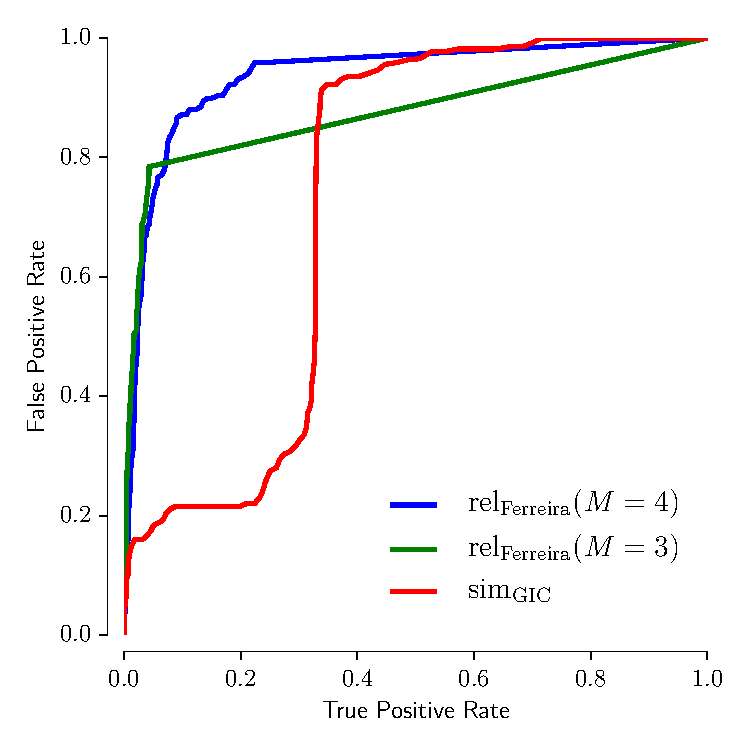
\includegraphics[width=0.8\textwidth]{images/roc.pdf}
    \caption[ROC analysis of the results of~$\ferreira$]{These ROC curves are the average over $10$~runs, each one produced with a different, randomly selected, negative set (\ie randomly selected pairs of \ontology{FMA} concepts).}
    \label{fig:roc}
\end{figure}

As is evident from this figure, $\ferreira$ shows a better performance than $\sim[GIC]$, since high values of TPR are obtained for low values of FPR. The main difference between $\ferreira$ with $M=4$ and~$M=3$ is that the former has more resolution power in that it can differentiate between concepts $8$~properties apart, whereas in the latter concepts with a path distance greater than~$6$ have automatically a relatedness value of~$0.0$. Thus, the measure calculated for many of the negative pairs in the dataset and also some of the positive ones ended up being~$0$. Given the lower resolution of the measure for~$M=3$, more pairs in this setting have relatedness~$0.0$, resulting in the straight diagonal line that we see in the figure.

Additionally, $\sim[GIC]$ does not perform as well as the relatedness measure. The distinct form of the graph occurs because a majority of the positive pairs (\ontology{FMA} concepts implicated in the same disease) are not really similar but simply related, just as in the example above: \term{Heart} and \term{Aortic valve} are relatively frequently implicated in the same disease, and their relatedness is high, as one is part of the other; on the other hand similarity measures are unable to capture this, since one is an organ and the other a valve, two distinct concepts.

This demonstrates the superiority of semantic relatedness measures over semantic similarity, at least when applied to ontologies where there is a vast number of properties, such as \ontology{FMA}, an in contexts where relatedness is more important than mere similarity.


\subsection{Conclusions and future work}

The most important conclusion to take from this work is that measures of relatedness can, in some cases, be more accurate than state-of-the-art measures of similarity, suggesting that relatedness measures do indeed play a role in the biomedical domain, especially when the expressiveness of the relevant ontologies (as measured by the number of properties) is as high as in this case.

The measure that I propose here is based on the concepts of \emph{semantic neighbourhood} and \emph{relevance factors}, and can accommodate the needs of particular applications by fine tuning its parameters. For example, by giving different weights to different properties, the measure can give more importance to some neighbours than others. Machine-learning algorithms can be used to tune the weight of each property according to the needs of each application.

The concept of relevant neighbourhood introduced in this work is also a bridge to other methodologies, particularly in allowing the use of ontology mappings to define wider neighbourhoods that draw not only from a specific ontology but from related ontologies as well, as long as a mapping of some sort exists between them. For example, cross-references can be used for this effect. In this context, the measure can incorporate external knowledge, but is not required to do so. For example, the semantic neighbourhood of a disease can include its symptoms and known treatments; to find the neighbourhood of enzymes, it is possible to include the chemical compounds that they transform; \etc.

Finally, the analysis preformed here on \ontology{FMA} shows that this is a valid method to measure relatedness between biomedical concepts. As we will see later, I have successfully applied this measure to other ontologies and other datasets (see \chpref{chap:multidomain}).


\section{Summary} \label{sec:enhancements/summary}

This chapter delineates my efforts in incorporating OWL axioms other than hypernymy into semantic measures. The first section deals with disjointness axioms while the second with existential quantification axioms. While this is by no means a comprehensive approach to using OWL formalism in semantic similarity, it paves the way for future experimentation and research in this context. As argued by \citet{Couto2013}, increasing the amount of such constructions used in semantic similarity calculations will eventually improve the overall panorama in this field of research and, therefore, the utility of this technique. As such, the results presented here are one of my major contributions to the area of semantic similarity and relatedness.

Even though these results do not directly support the idea of multiple-ontology semantic similarity, they were invaluable to the whole corpus of research that I was committed to achieve. In fact, they represent real scientific advances. Additionally, although $\ferreira$ was not originally validated in a multi-domain context, it can be easily converted into a measure that is able to tackle that problem, as we will see in \chpref{chap:multidomain}, by allowing the semantic neighbourhood of concepts to be generated based on several ontologies.

\chapter*[Interlude]{Interlude}

At this point in the document, it can perhaps benefit the reader to make a small summary of what has been discussed so far and how I continue to delineate my scientific contributions.

Multi-domain semantic similarity is useful to compare resources whose description spans several domains of knowledge, and biomedical informatics is rich in such resources: \eg epidemiological surges can be described using diseases, symptoms, pharmaceutical drugs, geographical locations, \etc. Comparison of these resources is important to enable searching capabilities on the multidisciplinary datasets, while allowing a certain kind of ``fuzziness'' on this search (resources need not fully satisfy a user query but can, instead, be similar to it).

Semantic similarity has been traditionally developed for single ontologies. As of June~2015, some published works deal with the multi-ontology problem, but all of them use multiple ontologies of the \emph{same domain} of knowledge, in an attempt to complement the knowledge in one ontology with the knowledge in another. Multi-\emph{domain} semantic similarity, in opposition, is important to compare multi-domain resources, annotated with concepts not only form distinct ontologies but from different fields of knowledge. No published literature deals with this problem, as far as I know.

As such, multi-domain semantic similarity measures need to be developed and validated. This is the research focus which this document reports. On the one hand, we can use single-ontology measures to compare concepts from one entity with ``compatible'' concepts from the second entity, thus obtaining a set of similarity values that can be mathematically aggregated into a single similarity value (aggregative approach); on the other hand, we can integrate all the relevant ontologies in a single knowledge-base and use existing measures directly on top of it (integrative approach).

This multi-faceted task will be described in the next three chapters. \chpref{chap:data} describes three multidisciplinary datasets collected to serve as test cases for multi-domain semantic similarity. The multi-domain measures (aggregative and integrative approaches) are presented in \chpref{chap:multidomain}, along with their associated results, stemming from its application over the three datasets. Finally, \chpref{chap:technical} will examine the technical details of semantic similarity, with particular focus on an open-source software suite that I developed to assist in calculating semantic similarity using OWL ontologies.


\chapter{Multi-domain data} \label{chap:data}

Although there is a need for multi-domain semantic similarity measures in the generality of the semantic web community, specifically within the scientific community, there is still a lack of substantial data this technique can be applied to. This, it can be argued, seems a contradictory state of affairs. Either there is data and as such the techniques to analyse them are needed, or there is a lack of data and the techniques are superfluous.

The truth is that semantic similarity is not a \emph{pressing} need for state-of-the-art semantic web practices, nor is it fundamental to \emph{current} scientific progress. In generic areas of the semantic web (outside the biomedical scope), ontologies are not even highly used, and knowledge is not \emph{well} represented, by which I mean
\begin{paralist}
    \item that ontologies are not consistent, either internally or with the external world;
    \item that the represented knowledge is severely incomplete; or
    \item that there is no way to integrate that knowledge with other ontologies, since the principles of interoperability are overlooked or neglected.
\end{paralist}
For example, \texttt{dbpedia.org}~\citep{Bizer2009a} is a collection of information spanning most domains of knowledge (based on the structured information of Wikipedia), but it is particularly rich in instance-level properties, not in ontological knowledge: while it contains the information that ``Lisbon'' \prop{has-timezone} ``Western European Time'', there is no representation of geospatial knowledge, which would, in particular, contain the axiom that \prop{has-timezone} is a property that can be applied to instances of \term{Place} and whose value must be a \term{Timezone}. Nevertheless, there is a small number of ontological information expressed in OWL, such as ``\term{Capital} \prop{is-a} \term{City}''.\looseness=-1

In contrast, while some areas of research, particularly in biomedical domains, are developing an increasing number of ontologies, there is still a lack of data annotated with them. One notable exception is the Gene Ontology, which is extensively used to annotate proteins and the results of genomic experiments (see \secref{sec:concepts/semantic-annotation} and \chpref{chap:validation}). This exception suggests that the lack of data does not correspond to a fundamental characteristic of scientific knowledge; instead, I argue that there is no motivation to annotate in the first place because there are not many tools able to explore the data. Once these tools start to appear, more data will be emerge. In light of this, one of the tasks I executed was multi-domain semantic annotation acquisition. These data allow the application of similarity measures on real datasets.

In this section, I present three datasets that were collected for exploiting semantic similarity, in three different areas of research: epidemiology, metabolism, and computational modelling of biological processes. For a list of the ontologies used by these datasets, see \appref{app:ontologies}.


\section{Epidemiology Dataset} \label{sec:data/epiwork}

Epidemiology is inherently a multidisciplinary subject, relying on areas of knowledge as diverse as medicine, biology, statistics, sociology and geography~\citep{Porta2008}. Even under the scope of medicine and biology, epidemiology deals with chemical compounds, diseases, symptoms, environmental conditions, methods of transmission, vaccines, \etc.

Given this multitude of domains, processing, storing and preserving epidemiological data is not straightforward. To explore ways of managing this type of data, a consortium of several partners established the Epiwork project, aimed at developing the appropriate framework of tools and knowledge to design epidemic forecast infrastructures, including an epidemiology data repository that was developed by the LaSIGE partner (see \secref{sec:auxiliary-projects/epiwork} for a summary of my contributions to the Epiwork project).

One of the most important functions of a data repository is the ability to search within its resources. A search box that can be used to convert a user query into a list of results is essential for the widespread adoption of the repository. There are at least two possible ways to implement this feature:
\begin{paralist}
    \item allow free text searches that try to map the words in the query to the words in the content of each resource; or
    \item annotate the resources of the repository with metadata that reflect its content and use the query to search within these metadata.
\end{paralist}
While the first way maps roughly to how web search engines work today, the second way is much more aligned with the idea behind the semantic web, with all its advantages (see \secref{sec:concepts/semantic-annotation,sec:concepts/semantic-web}) and, as such, the team behind the Epidemic Marketplace decided to provide a way for users and curators to annotate their resources.

Given the multidisciplinary nature of epidemiology and the resources contained in the Epidemic Marketplace, a multi-domain semantic similarity measure would be an asset to assist the search functionality, which would require a means to compare resources based not on one domain in particular (\eg diseases), but on all the domains of annotation.

Consider a user searching for resources about ``infectious diseases''. Using the Human Disease Ontology (\ontology{DOID}), specifically its class-subclass hierarchy, the search functionality can successfully retrieve all resources with data on \term{Flu}, \term{AIDS} and other infectious diseases. However, it can happen that the user queries for very specific resources (for example by over-specifying the disease, the symptom or the location of an outbreak), resulting in an empty list of retrieved resources. In such cases, it is possible to find some results that \emph{almost} satisfy the query by comparing the repository resources with the query. For example, the query ``2009~European infectious disease outbreaks that manifest through coughing'' could be satisfied with a resource about a 2010~European infectious disease outbreak that manifested through sneezing. Additionally, when the query does return some results, semantic similarity can be used to sort those results according to how related they are to the original query.

On the other hand, semantic similarity provides a mechanism to implement a ``Related resources'' section in the repository. Users looking at the contents of a particular resource are usually interested not on a single resource but on a collection of them, all of which are related. For example, a user looking at a resource that contains data about flu-like diseases is probably also interested in resources about other infectious pulmonary diseases. Having a section of the web page dedicated to these related resources removes the need for the user to make complex and sometimes unintuitive queries to the search feature.

One of my contributions to this project was the development of a semantic metadata model and a Network of Epidemiology-Related Ontologies (NERO). Both are used to assist the annotation of epidemiological resources: the metadata model describes the type of information that a resource needs and NERO provides concepts for the annotation (see \secref{sec:auxiliary-projects/epiwork}).

During the Epiwork project, it was possible to annotate a set of $228$~resources, each one containing a reference to an open-access paper from an epidemiology journal (the annotation process itself was conducted by someone else in the project, not me). Each of these resources is annotated with a set of concepts from NERO according to the semantic metadata. Hence, this dataset contains metadata on domains such as ``environment'', ``diseases'', ``symptoms'', ``modes of transmission'', ``demography'' \etc.

By leveraging on NERO to represent the concepts that each paper refers to, the papers become enriched with semantic information and can, therefore, be used in semantic analysis. While there is no explicit quantitative assessment of similarity or relatedness between these resources, and as such there is still no gold-standard that can be explored in the development of multi-domain semantic similarity, doing so is not beyond the realm of possibilities, since the resources are already annotated. As such, I gathered this dataset to run semantic similarity on it, as we will see later in \chpref{chap:multidomain}.

A summary of the relevant annotations for these resources is given in \tabref{tab:epiwork-summary}. In this table, I make use of three statistics that depict the annotation panorama of these resources with respect to a single domain:
\begin{description}
    \item[Coverage] This is the fraction of resources that have at least one annotation in the domain.
    \item[Volume] This is the average number of concepts from this domain in the resources. It is calculated with respect to the resources that have at least one annotation, which means that the minimum value is~$1.0$.
    \item[Diversity] This is the number of distinct concepts from the domain that are used throughout all the dataset.
\end{description}

\begin{table}
\caption[Summary of the annotation in the epidemiology dataset]{This dataset corresponds to $228$~epidemiology resources extracted from the Epidemic Marketplace. The first two columns describe the domains and ontologies used to annotate the resources. The rest of the columns provide statistics for each domain. A description of each statistic is given in the text.}
\label{tab:epiwork-summary}
\centering
\small
\begin{tabular}{llrrr}
\toprule
\textbf{Domain} & \textbf{Ontology} & \textbf{Coverage} & \textbf{Volume} & \textbf{Diversity} \\
\midrule
Chemistry    & \ontology{CHEBI} &   0.9\% & 1.00 &   1 \\
Diseases     & \ontology{DOID}  &  59.6\% & 1.76 &  70 \\
Environment  & \ontology{ENVO}  &  21.1\% & 1.00 &   9 \\
Phenotypes   & \ontology{PATO}  &   0.9\% & 1.00 &   1 \\
Symptoms     & \ontology{SYMP}  &  46.1\% & 3.55 &  79 \\
Transmission & \ontology{TRANS} &  42.5\% & 1.00 &   9 \\
Vaccines     & \ontology{VO}    &  20.6\% & 1.06 &  16 \\
General      & \ontology{NCIt}  & 100.0\% & 4.13 & 157 \\
General      & \ontology{MeSH}  &  83.8\% & 2.24 & 131 \\
\bottomrule
\end{tabular}
\end{table}


\section{Metabolic Pathways Dataset} \label{sec:data/pathways}

Another multidisciplinary area in the field of biomedical informatics is metabolism. This field studies the chemical reactions that take place in a living organism and which are the basis of biology and life in general. For example, it studies how the energy of sunlight is used by plants and other organisms to convert water and carbon dioxide into oxygen and glucose, a process known as photosynthesis. A full description of such a process is called a \emph{metabolic pathway}, which is often depicted as a graph showing the intervening molecules.

The process described by a metabolic pathway is usually performed inside a cell, or within its immediate surroundings, with the assistance of enzymes (proteins that accelerate the chemical reactions), and it has certain chemical inputs and outputs. Metabolic pathways encompass several smaller steps (the individual chemical reactions) and several intermediary molecules, such as the metabolites (the molecules that are transformed), the enzymes, and other regulatory proteins that supervise the whole process based on cellular conditions (such as the amount of oxygen within the cell, the amount of sunlight, \etc.). \figref{fig:pathway} contains a simple example of a metabolic pathway involving several metabolites and enzymes.

\begin{figure}
    \centering
    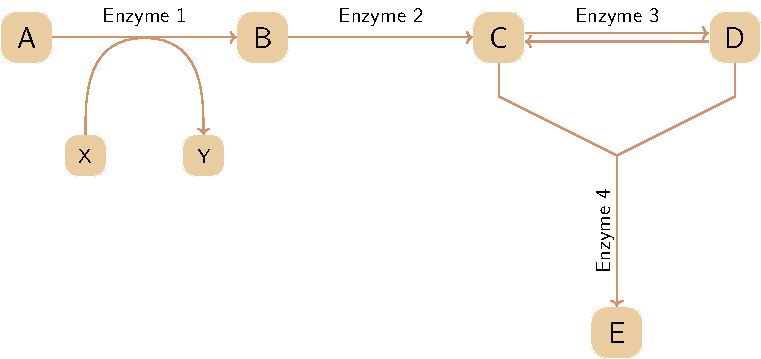
\includegraphics{images/pathway.pdf}
    \caption[Example metabolic pathway]{This figure illustrates a hypothetical metabolic pathway. Chemical reactions are catalysed by specialised proteins known as enzymes, which accelerate the rate at which metabolites are converted. The image depicts that some reactions require extra metabolites, and other produce extra chemical compounds. The pointed arrows represent the ``flow of matter'', \ie the fact that one metabolite is converted to another one, thus implicitly describing the input and output of the pathway. In this case, the inputs are the metabolites \term{A} and~\term{X}, and the outputs are the metabolites \term{E} and~\term{Y}.}
    \label{fig:pathway}
\end{figure}

While these chemical reactions usually occur within living organisms as a continuum, \ie there is no naturally defined boundary between metabolic pathways, dividing the high amount of distinct chemical reactions into manageable groups simplifies the study of metabolism. For example, the glucose produced by photosynthesis, in plants, is converted into other molecules, but even though the two processes happen simultaneously, each is described by a distinct pathway.

Knowing the components of a metabolic pathway and how they interact with one another is extremely helpful:
\begin{paralist}
    \item a metabolic pathway is a means of effective communication regarding the metabolism of various organisms~\citep{Papin2003};
    \item it enables the mathematical analysis of a complete metabolic system, since they correspond to precise mathematical descriptions of cellular properties~\citep{Papin2003}; and
    \item this information can provide insight into how organisms respond to failures in the pathway (such as the absence of an enzyme)~\citep{Baumgartner2011}.
\end{paralist}
Furthermore, inside cells, many different processes occur at the same time, with thousands of molecules being converted concurrently. As such, to quickly estimate the effect of changing something in a pathway, assistance from computerised system is required.

What makes metabolic pathways multidisciplinary is the fact that, to fully describe them, we need not just the metabolites that are converted and the molecular functions that are carried out, but also the drugs that interfere with the pathway and the diseases caused by pathway defects or other malfunctions. The Kyoto Encyclopedia of Genes and Genome (KEGG \mdash \url{http://www.genome.jp/kegg/kegg2.html}) is a collection of databases on biological systems. One of these databases is \kegg{pathway}, which categorises $269$~pathways into a hierarchy, and annotates each pathway with:
\begin{paralist}
    \item chemical compounds,
    \item enzymes,
    \item drugs that affect the pathway, and
    \item diseases that are associated with the pathway.
\end{paralist}
Annotation is done with concepts from other KEGG databases. The concepts linked to in these annotations are not from the reference ontologies mentioned in \appref{app:ontologies}, but conversion to \ontology{GO} and \ontology{CHEBI} can be performed, using KEGG's own internal tables, which map compound and drug concepts to \ontology{CHEBI}, and genes to UniProt identifiers (which can be used to find \ontology{GO} annotations for the genes). Diseases, however, have no link to reference ontologies. As such, an additional step was executed to convert KEGG diseases into Human Disease Ontology (\ontology{DOID}) identifiers.
% \appref{app:kegg-conversion} contains a detailed description of this conversion process.

\tabref{tab:pathways-summary} shows a summary of the annotations for these pathways, using the same statistics presented for the previous multi-domain dataset. Notice that in this dataset, there is not a one-to-one correspondence between domains and ontologies, since both drugs and metabolites are represented as \ontology{CHEBI} concepts. I decided to keep the two domains separate since they encode different information about the pathways.

\begin{table}
\caption[Summary of the annotation in the metabolic pathways dataset]{This dataset corresponds to $269$~pathways extracted from KEGG. Note that a domain in this dataset does not precisely correspond to an ontology, as both drug and metabolite annotations use concepts from \ontology{CHEBI}. The first two columns describe the domains and ontologies used to annotate the resources. The rest of the columns provide statistics for each domain.}
\label{tab:pathways-summary}
\centering
\small
\begin{tabular}{llrrr}
\toprule
\textbf{Domain} & \textbf{Ontology} & \textbf{Coverage} & \textbf{Volume} & \textbf{Diversity} \\
\midrule
Diseases            & \ontology{DOID}  &  79.2\% &  9.08 &  756 \\
Drugs               & \ontology{CHEBI} &  42.4\% & 30.30 & 1381 \\
\ontology{GO} terms & \ontology{GO}    & 100.0\% & 32.45 & 3210 \\
Metabolites         & \ontology{CHEBI} &  79.9\% & 21.37 & 2628 \\
\bottomrule
\end{tabular}
\end{table}

Like in the case of epidemiology resources, a database of pathways needs a multi-domain semantic similarity measure to be able to properly make use of all the information available about each pathway in order to answer user requests with the most relevant resources. Additionally, semantic similarity in metabolic pathways can also be used to
\begin{paralist}
    \item reconstruct phylogenetic trees depicting the common metabolic history of a group of organisms~\citep{Heymans2003a}, and
    \item find suitable model organisms in the study of diseases related to a certain metabolic condition~\citep{Forst1999}.
\end{paralist}
Single-ontology semantic similarity has been researched in this domain by \citet{Clemente2005}, which used similarity of proteins based on their \ontology{GO} annotations, and \citet{Grego2010}, which used instead semantic similarity between the metabolites of the pathways based on \ontology{CHEBI}.

By gathering metabolic pathway information in this way, I effectively created a dataset of pathways annotated with \ontology{CHEBI}, \ontology{GO} and \ontology{DOID} concepts, which was further used in semantic similarity studies (see \chpref{chap:multidomain}).


\section{Biochemical Models Dataset} \label{sec:data/biomodels}

A third area where multi-domain semantic similarity can be of service corresponds to models of biological systems, or biomodels, for short. This type of information is similar to the one of the previous dataset: like a metabolic pathway, a biomodel is a description of a chemical process that happens inside the cell, or within its immediate surroundings. In contrast, however, a biomodel is more computationally oriented. It represents the metabolites and enzymes involved in the reactions but also the cellular components and anatomical location where they occur, including their volume, and the equations that describe the reaction velocity with respect to the concentration of the metabolites and enzymes.

Like in the previous two scenarios, multi-domain semantic similarity is useful here as well, primarily to enable searching capabilities within a database of biomodels. Other applications include
\begin{paralist}
    \item clustering the biomodels according to similarity in order to find common patterns in different organisms, which can be used to transfer knowledge from one organism to another; and
    \item using semantic similarity to assist the act of annotating the models, by analysing similar biomodels and generating new annotation suggestions to increase the accuracy of the annotations given by an author~\citep{Schulz2012}.
\end{paralist}

The EBI Biomodels Database (\url{http://www.ebi.ac.uk/biomodels-main/}) contains formal descriptions of mathematical models of biochemical systems~\citep{Li2010a,Juty2015}. These biomodels are annotated with concepts from the relevant domains, including chemical compounds, enzymes, biological processes and anatomical entities.

% For example, the biomodel that represents the complement system~\citep{Liu2011}, a part of the immune system, includes annotations to:
% \begin{itemize}
%     \item \term{N-Acetyl-D-glucosamine} and \term{Phosphocholine} (chemical compounds);
%     \item \term{Portion of plasma} and \term{Extracellular region} (anatomical locations);
%     \item \term{Dendrite} and \term{Mitochondria} (cellular locations);
%     \item several proteins (such as \term{Uniprot:P01024}) that are responsible for performing the functions of this system and which have themselves \ontology{GO} annotations based on their functions.
% \end{itemize}

The models in this dataset are annotated with the reactions that they represent, the chemical compounds involved in the reactions (both metabolites and enzymes) and the cellular components where the reactions occur. This information is frequently (but not always) accompanied with links to ontologies such as \ontology{GO} and \ontology{CHEBI}. For example, reactions are linked to concepts from \ontology{GO}; chemical compounds are linked to \ontology{CHEBI} concepts, \kegg{compound} terms, and InterPro and UniProt identifiers; protein complexes that participate in the reaction and cellular components are linked to the Cellular Component branch of \ontology{GO} (which represents complexes as well as membrane-delimited components); cell components are also linked to \ontology{FMA} concepts; and physical quantities, like mass and electric charge, are linked to \ontology{PATO} concepts.

Given the complexity of these annotations, I decided to make some conversions and ignore some annotations. For example, I ignored \kegg{protein} terms (there are only~$3$ in the whole set of annotations). \kegg{compound} terms were converted to \ontology{CHEBI} concepts when possible (compounds without a correspondence were ignored as well), and UniProt and InterPro identifiers were converted into the \ontology{GO} annotations for those proteins. This resulted in each model having annotations to \ontology{CHEBI}, \ontology{FMA}, \ontology{GO} and \ontology{PATO}. A summary of the annotations for the biomodels is given in \tabref{tab:biomodels-summary}.

\begin{table}
\caption[Summary of the annotation in the biomodels database]{This dataset corresponds to the $282$~distinct biomodels extracted from the BioModels website. The first column describes the ontologies used to annotate the resources. The rest of the columns provide statistics for each ontology.}
\label{tab:biomodels-summary}
\centering
\small
\begin{tabular}{lrrr}
\toprule
\textbf{Ontology} & \textbf{Coverage} & \textbf{Volume} & \textbf{Diversity} \\
\midrule
\ontology{CHEBI} & 55.0\% &  6.99 &  261 \\
\ontology{FMA}   &  3.9\% &  1.18 &   11 \\
\ontology{GO}    & 90.8\% & 55.43 & 3314 \\
\ontology{PATO}  & 95.4\% &  1.06 &    5 \\
\bottomrule
\end{tabular}
\end{table}

I extracted from this dataset $250$~pairs of biomodels (for a total of $282$~distinct biomodels), with the aim of having a Systems Biology expert assess the degree of similarity between each pair. The data in this \emph{gold-standard} corresponds to the models and their annotations from the corresponding ontologies. To ensure a good coverage of all similarity values, $100$~pairs were generated randomly and the other~$150$ were generated based on a preliminary semantic similarity calculation, in order to have a balanced distribution of similarity values. To this effect, I first calculated semantic similarity on all the biomodel pairs and divided the pairs into three categories: one for similarity values below~$0.33$, another for values between $0.34$ and~$0.67$, and another for values higher than~$0.67$. This ensured that pairs covering the full range of similarity were included in the gold-standard. The $100$~random pairs were generated to cover the possibility that the preliminary similarity values were not significant.

The $250$~pairs were classified by the expert as ``not similar'', ``somehow similar'', ``similar'', and ``very similar''. Expert assessment was conducted based on a web-tool that I designed for that effect. \figref{fig:biomd} displays some screen-shots of the tool.

\begin{figure}
    \centering
    \subbottom[The main page of the similarity assessment tool%
               \label{fig:biomd/page}]{%
        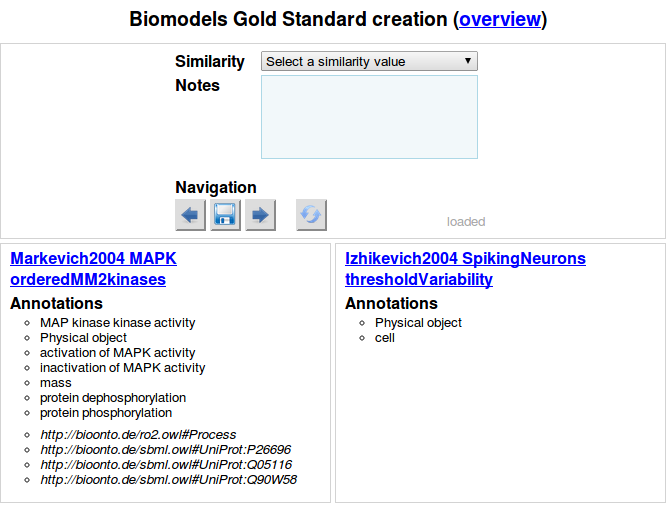
\includegraphics[scale=0.55]{images/biomd-page-2.png}%
    }
    \vspace{\baselineskip}
    \subbottom[A detail of the similarity selection section%
               \label{fig:biomd/detail}]{%
        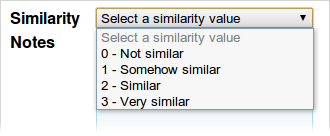
\includegraphics[scale=0.55]{images/biomd-detail.png}%
    }
  
    \caption[The EBI Biomodels similarity assessment tool]%
    {\subcaptionref*{fig:biomd/page} Each model is accompanied with the set of ontology concepts that annotate it. In the bottom of this panel, there are control buttons to navigate through the $250$~pairs and a ``Notes'' section to allow the expert to make their own notes, for future reference. \subcaptionref*{fig:biomd/detail} The similarity value can be chosen between $0$ and~$3$.}
    \label{fig:biomd}
\end{figure}

\chapter{Multi-domain semantic measures} \label{chap:multidomain}

\begin{note-paper}
    This chapter is adapted from a papers submitted to Oxford Bioinformatics in December 2015, and is still waiting its first round of peer-review reports.
\end{note-paper}

Given the multidisciplinarity of biomedical resources, it is necessary to implement measures of similarity that can handle all the relevant domains. For instance, to compare metabolic pathways one can use protein similarity~\citep{Clemente2005} or chemical similarity~\citep{Grego2010}, but we can also conceive a scenario where both sources of knowledge are important and, therefore, where comparison needs to explore the two domains. In theory, this should provide a more accurate insight into what the pathways represent in the real world and, ultimately, contribute to a better similarity measure.

In this chapter, I propose the hypothesis that multi-domain semantic similarity has some advantages compared to classical single-ontology measures when dealing with multidisciplinary resources; in particular, I demonstrate this hypothesis based on the accuracy of both techniques in the three different datasets presented in \chpref{chap:data}. By doing so, I also show that multi-domain measures are necessary for the advancement of science and that, as time passes and the amount of resources annotated with concepts from multiple ontologies increases, the demand for such measures will also increase.

Given the success of single-ontology semantic similarity measures in the past, instead of a new measure of semantic similarity built from scratch, I propose two mechanisms that \emph{lift} single-ontology measures into their multi-domain counterparts: the \emph{aggregative approach} compares each of the domains of relevance independently and then aggregates the several similarity values into a final score; and the \emph{integrative approach} integrates all the ontologies under the same common root and then applies single-ontology measures on it.

\newpage

\section{The two multi-domain approaches} \label{sec:multidomain/approaches}

Multidisciplinary entities are commonly annotated in domains that are on a one-to-one correspondence with a set of ontologies, since biomedical ontologies tend to represent a specific domain of knowledge, per the guidelines of the biomedical informatics community (see \secref{sec:concepts/ontologies} and \appref{app:ontologies}). For example, concepts used to annotate epidemiology resources include diseases from \ontology{DOID}, symptoms from \ontology{SYMP}, vaccines from \ontology{VO}, \etc. Sometimes, the same ontology corresponds to more than one domain (\eg in metabolic pathways, annotations to \ontology{CHEBI} are used both for metabolites and drugs, and \ontology{GO} annotations for molecular functions, biological processes and cellular components); the reverse is not as common (more than one ontology annotating for the same domain).

My work assumes that dividing the annotations in domains can be done in a straightforward way (\cf the datasets described in \chpref{chap:data}, where such division is presented in those chapter's tables). It also assumes the existence of a group-wise single-ontology semantic similarity measures which can compare a set of concepts with another set of concepts, examples of which include:
\begin{itemize}
    \item concept-wise similarity measures, such as $\sim[Resnik]$~(\eqref{eq:resnik-ssm}) and $\sim[Lin]$~(\eqref{eq:lin}), which can be made group-wise with the use of an aggregation technique, as described in \secref{sec:sota/annotated}; and
    \item measures that are inherently group-wise, like $\sim[UI]$~(\eqref{eq:simui}), $\sim[GIC]$~(\eqref{eq:simgic}) and $\ferreira$~(\eqref{eq:ferreira}).
\end{itemize}

The following subsections describe the two approaches that lift single-ontology measures into multi-domain measures.


\subsection{Aggregative approach} \label{sub:approaches/aggregative}

This approach treats each domain of annotation independently. For each annotation domain, the concepts of that domain used to annotate the first entity are compared to the concepts of that domain used to annotate the second entity, using the group-wise single-ontology measure. This produces a collection of similarity values, one for each domain, which must then be aggregated with the use of a function such as the maximum, the minimum or the average. See \figref{fig:aggregative} for a graphic illustration of this process.

While the aggregation technique can be one of several different options, I show here only the results of two of them: the raw average and the weighted average. Let $e$ and~$e'$ be two multi-domain annotated entities being compared, $e_d\,$ and~$e'_d\,$ be the set of concepts annotating the entities $e$ and~$e'$ in the domain~$d$, $D$~be the set of all domains annotating the two entities, and $\sigma$~be the single-ontology semantic similarity measure being lifted. I define
\begin{eqnarray}
    \sim[Aggr_{raw}](e, e') &=&
    \frac{1}{N} \cdot
    \sum_{d \in D} \sigma(e_d, e'_d)
    \label{eq:sim-aggr-raw} \\
    %
    \sim[Aggr_{weighted}](e, e') &=&
    \frac{1}{\sum_{d \in D} w_d} \cdot
    \sum_{d \in D} w_d \cdot \sigma(e_d, e'_d)
    \label{eq:sim-aggr-weighted}
\end{eqnarray}
where $w_d$~is the weight associated with the domain~$d$. I followed an approach that weights each domain by the amount of annotations that it provides to the entities being compared; as such, domains that are more represented in an entity contribute with a higher weight to the final similarity value:
\begin{equation}
    w_d = \left\vert e_d \cup e'_d \right\vert.
\end{equation}
For example, if a domain contributes to the annotations of $e$ and~$e'$ only with one concept (either only to one of the entities or to both), the weight of this domain will be~$1$. Domains that contribute with a higher number of concepts have a higher weight on the overall similarity value.

\begin{figure}
    \centering
    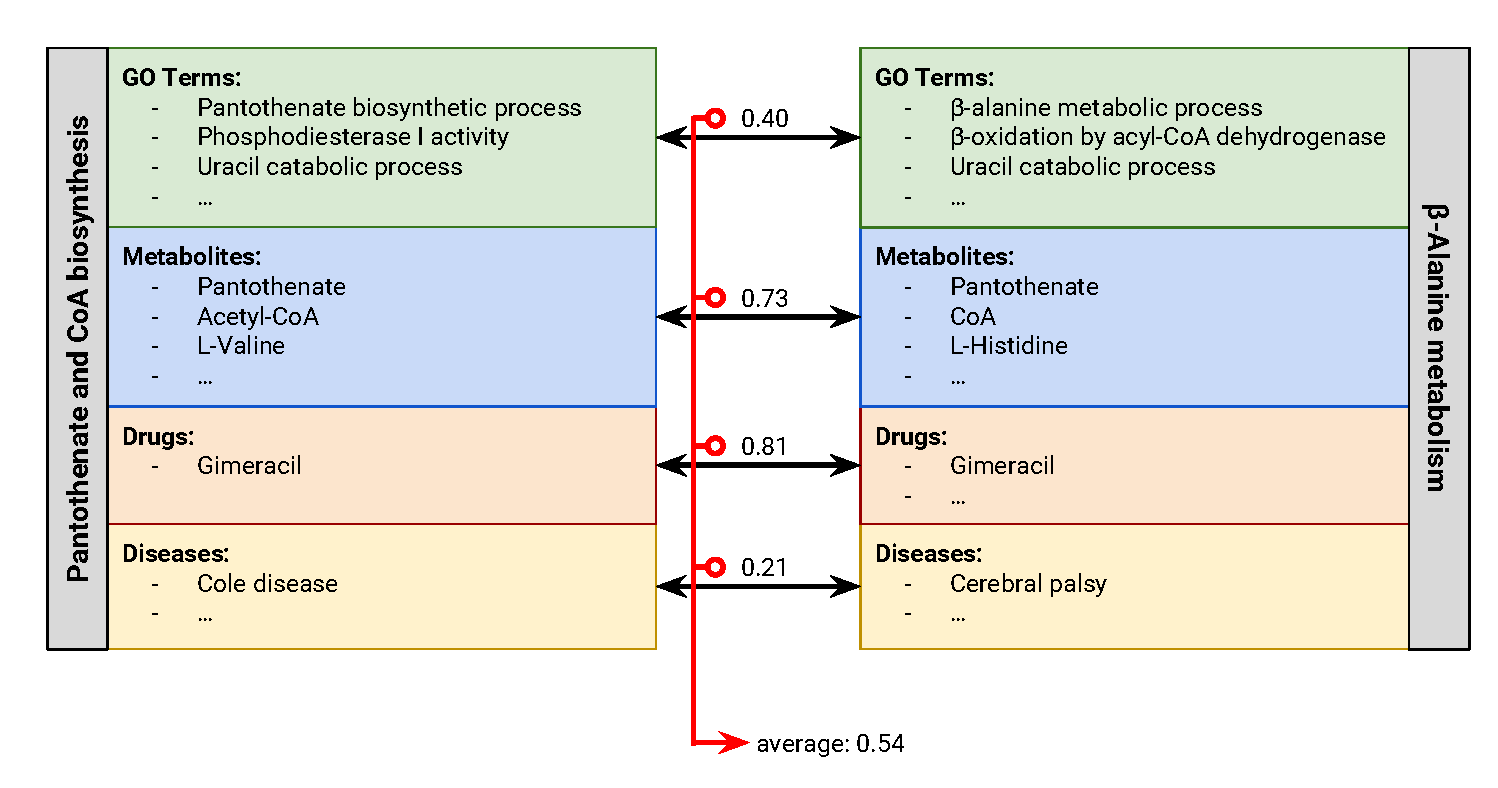
\includegraphics[width=\linewidth]{images/multi-aggregative.pdf}
    \caption[The aggregative approach]{This image illustrates how this mechanism works using two metabolic pathways as example. Each domain is identified by colour. The concepts in each domain in the first entity are compared to the concepts in the same domain in the second entity, and then the values are aggregated; in this example, the aggregation mechanism was the raw average.}
    \label{fig:aggregative}
\end{figure}

This method has the advantage that it can directly use existing measures to compute similarity and works irrespective of the degree of interoperability between the various ontologies used to annotate the entities.


\subsection{Integrative approach} \label{sub:approaches/integrative}

While one of advantage of the previous approach is the possibility to be applied to non-interoperable ontologies, biomedical ontologies are \emph{generally} interoperable in at least two ways:
\begin{itemize}
    \item the use of the Basic Formal Ontology (\ontology{BFO}) as an upper ontology~\citep{Grenon2004}, which means that concepts form different ontologies have the potential to share common superclasses (even if only general and abstract ones); and
    \item the use of cross-references between ontologies (\eg the link between a disease and the anatomical entities that it affects), which most ontologies in this field try to satisfy. This stems from the reuse of concepts from different ontologies (\eg \ontology{VO} reuses the concepts \term{Chemical entity} from \ontology{CHEBI} and \term{Protein complex} from \ontology{GO}), which enables ontologies to refer to concepts outside their domain but at the same time relevant for describing the knowledge of that domain.
\end{itemize}

In fact, by separating the various domains into independent groups, we lose information that could also be used to compute similarity. First, if only one of the entities is annotated in one domain, (\eg \ontology{FMA}), this domain is effectively ignored, and no amount of annotation can change that. Second, inter-domain relationships between concepts in different ontologies are also ignored. For example, an annotation to the concept \term{Deafness} cannot be correlated with an annotation to \term{Ear} or even \term{Hearing}, since those concepts are all part of different domains (they are, respectively, represented in, \ontology{DOID}, \ontology{FMA} and \ontology{NCIt}).

One way to avoid the pitfalls of separating the multiple domains in isolate computations is to merge all the relevant ontologies in a single multi-domain virtual ontology and then to use the single-ontology measure directly on top of this virtual ontology. This is the second approach, where all concepts of one entity are compared to all the concepts of the other (see \figref{fig:integrative}). Measures of this type assume, therefore, that there is interoperability between the ontologies being used. This is essential in two accounts:
\begin{itemize}
    \item in relatedness measures, it is vital, for example, that the molecular function \term{ATP binding} is explicitly related to the chemical compound \term{ATP}, since this relationship allows the relatedness measure to compute a high value for this pair of concepts;
    \item likewise, although the molecular functions \term{Ethanol degradation} and \term{Cellular response to ethanol}, both part of \ontology{GO}, are not fundamentally similar (one is the process by which the body converts ethanol to other smaller molecules, the other is the process that cells undergo in the presence of ethanol, and their most informative common superclass is the abstract concept \term{Physiological process}), both contribute to the metabolism of the same compound, and are similar in the sense that the two processes are related to \term{Ethanol}, a concept that is represented in a different ontology. Exploring this relationship can also increase accuracy of similarity.
\end{itemize}

\begin{figure}
    \centering
    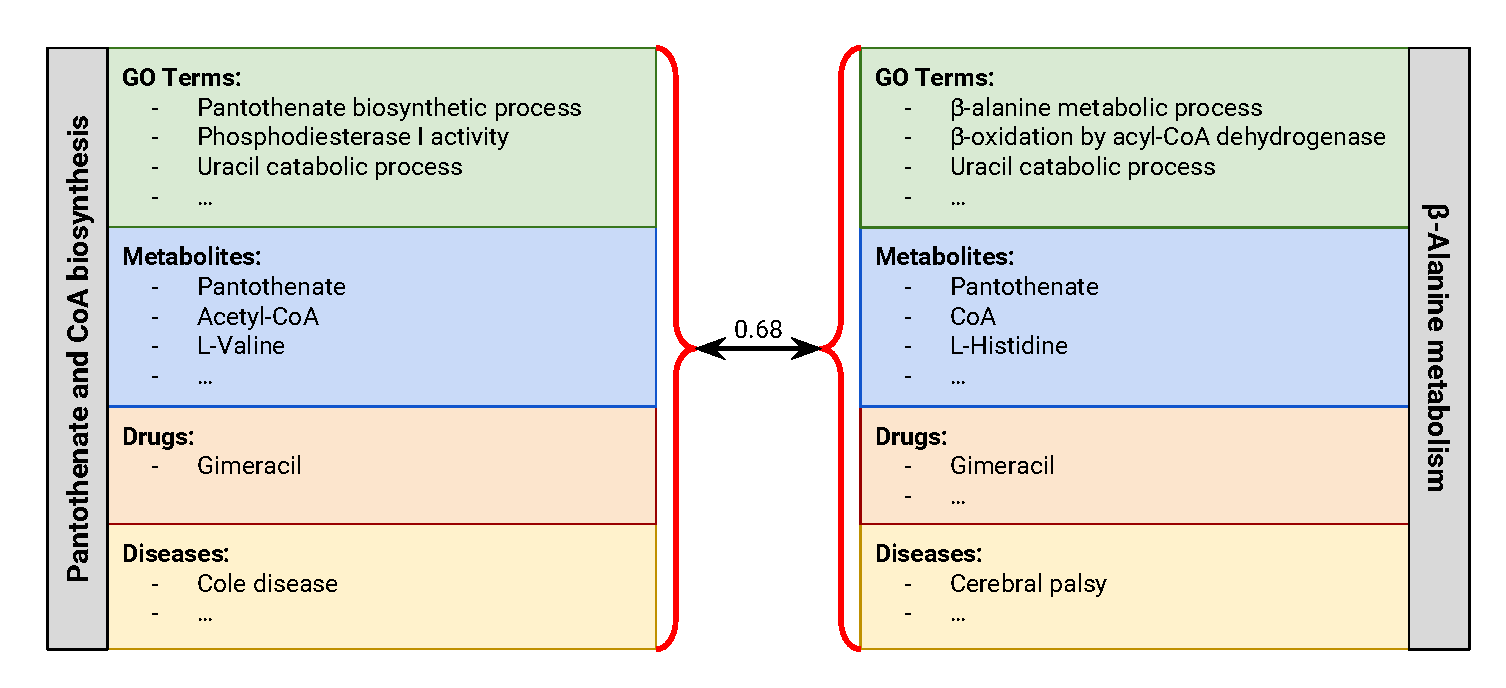
\includegraphics[width=\linewidth]{images/multi-integrative.pdf}
    \caption[The integrative approach]{All the ontologies are aggregated under the same root, which means that single-ontology measures can be directly applied to compare concepts from different domains. In this case, only one value is obtained, which corresponds to the semantic similarity value.}
    \label{fig:integrative}
\end{figure}

To achieve this, all the ontologies that are used must be in some way merged into a single knowledge representation artefact (a single ontology). Merging ontologies is a process that is mainly studied by Ontology Matching~\citep{Shvaiko2005,Euzenat2007}, and consists in automatically or semi-automatically finding the concepts that are equivalent in two ontologies. In the semantic web context (see \secref{sec:concepts/semantic-web}), ontology matching has a critical role, since it helps integrate heterogeneous entities, usually created by different research groups but with a certain overlap in their domains. However, there is a large effort to make biomedical ontologies interoperable, in the sense that
\begin{paralist}
    \item concepts are reused among ontologies to refer to the same real-world idea,
    \item there is a common upper level ontology, which represents the most abstract concepts and provides a common ontological background that enables an objective classification of concepts, and
    \item ontologies are orthogonal, thus each is responsible for representing exactly one domain of knowledge.
\end{paralist}
As such, ontology matching between reference ontologies in the biomedical domain is not expected to produce a high number of matches. In fact, since each ontology represents a different domain, there are, theoretically, no ``semantically equivalent'' concepts in any pair of reference biomedical ontologies (in practice, this is not exactly true, as some domains overlap \mdash \eg both \ontology{GO} and \ontology{FMA} contain the concept of \term{Cell}, represented with different identifiers \mdash but the amount of overlap is extremely small, it is decreasing as time goes by, and it is almost always relative to abstract rather than specific concepts).
\looseness=1

Therefore, in practice, biomedical ontologies that need concepts from other domains ``import'' those concepts from other ontologies. For example, many biological process concepts in \ontology{GO} represent biochemical reactions, and these concepts are appropriately linked to the \ontology{CHEBI} concepts that represent the molecules that are transformed in these reactions: \eg the concepts \term{Ethanol degradation} and \term{Cellular response to ethanol} mentioned above are linked to the concept \term{Ethanol} represented in \ontology{CHEBI}. These facts are asserted using existential quantification axioms (see \secref{sec:enhancements/relatedness}):
\begin{align*}
    \term{GO:``Ethanol degradation''} &
        \sqsubseteq\:\exists\,\prop{has-input}\,.\,\term{CHEBI:``Ethanol''}, \\
    \term{GO:``Cellular response to ethanol''} &
        \sqsubseteq\:\exists\,\prop{has-input}\,.\,\term{CHEBI:``Ethanol''}.
\end{align*}

Rather than ontology matching, it is these inter-domain cross-references that can potentially increase the accuracy of semantic similarity measures. With them, it becomes possible to find a specific rather than abstract connection between the \ontology{GO} concepts \term{Ethanol degradation} and \term{Cellular response to ethanol}, which was otherwise absent from the \ontology{GO} ontology. Measures such as~$\ferreira$ are capable of exploring the inter-domain cross-references and use them to compare ontology concepts (see \secref{sec:enhancements/relatedness}) and, by extension, annotated entities.

% For example, a mapping from diseases to frequently associated symptoms is useful when comparing entities associated with diseases \andor symptoms. One the one hand, this provides a means to directly measure relatedness between a disease and a symptom; on the other hand, similarity between diseases can also reflect the real world more accurately, since more information is added to the system and can be used for that comparison (\eg measures that are able to exploit this kind of information can assign a higher value to the similarity between diseases that share frequent symptoms, even if the diseases are otherwise not similar).

Unfortunately, the current state of cross-linking in biomedical ontologies is largely underdeveloped, despite it being a recommended practice by the OBO Foundry. The group responsible for developing and maintaining \ontology{GO} intends to provide cross-references to appropriate concepts from other ontologies. Examples already deployed are the ones given in the previous paragraph, which link \ontology{GO} and \ontology{CHEBI}. Planned links include cross-references to anatomical locations and species names~\citep{Mungall2011}. Furthermore, \ontology{HPO} represents human phenotype abnormalities, and links them to anatomical concept from \ontology{FMA}. For example, \term{Microtia} is defined as the ``Underdevelopment of the `external ear' (\ontology{FMA}:52781)''.

Incidentally, OWL is well suited to deal with this type of cross-reference. If two ontologies refer to the same identifier, when the ontologies are used together, that identifier will refer to the same concept; as long as all the necessary ontologies are loaded, these type of inter-domain axioms can be defined in one ontology using an identifier from another ontology, which makes this multidisciplinary fact directly available out of the box. This is because, in the semantic web, identifiers are universal, and always identify the same concept. For example, there is an OWL file representing \ontology{GO} that contains the axioms exemplified above, which relate molecular functions with chemical compounds. This file does not have any information about the \ontology{CHEBI} concepts other than the identifier. Therefore, an automatic system that needs more information on those \ontology{CHEBI} concepts, \eg its superclasses, name and synonyms, must load \ontology{CHEBI} to find it.


\section{Results} \label{sec:multidomain/results}

I have applied semantic similarity to the multi-domain datasets described in \chpref{chap:data}. As these are intrinsically multidisciplinary datasets, they provide an appropriate and highly relevant testbed to try the two approaches described above. I refer the reader to \tabref{tab:epiwork-summary} (page~\pageref{tab:epiwork-summary}), \tabref{tab:pathways-summary} (page~\pageref{tab:pathways-summary}) and \tabref{tab:biomodels-summary} (page~\pageref{tab:biomodels-summary}), describing the amount of annotations on these datasets, which will, therefore, be pertinent to the analysis presented here.

Except where otherwise stated, all the results presented in this section were obtained using $\sim[Resnik]$~(\eqref{eq:resnik-ssm}) as the group-wise single-ontology semantic similarity measure. Since this is a concept-wise measure, I used it to create a similarity matrix, where each value is the similarity between one of the annotations in the first entity and one of the annotations in the second entity, and then use a Best Match Average (BMA) approach to convert this matrix into a single similarity value. Other group-wise single-ontology measures have been used, in particular~$\ferreira$, with results equivalent to the ones presented. As such, these results are not shown, except where relevant. In particular, although some measures are better suited to tackle some problems than other measures (for example, a measure that uses disjointness axioms is better suited to deal with problems related to \ontology{CHEBI} concepts, as detailed in \secref{sec:enhancements/disjointness}), the increase in performance observed in multi-domain semantic similarity over single-ontology semantic similarity is largely independent of the group-wise measure used with it.

For each case study, I used semantic similarity in four different settings:
\begin{description}
    \item[Baseline] This is a collection of measures instead of a single one. Each measure compares only the concepts from one domain and completely disregards the other domains. This corresponds to the classical single-ontology measure and serves as a baseline to determine whether multi-domain measures outperform single-ontology measures.
    \item[Aggregative (raw)] This setting corresponds to the aggregative approach, with all the single-ontology values obtained in the baseline setting being averaged with equal weights~(\eqref{eq:sim-aggr-raw}).
    \item[Aggregative (weighted)] This is the same as last setting, except that the average of the various values is weighted in proportion to the number of annotations in each domain~(\eqref{eq:sim-aggr-weighted}).
    \item[Integrative] This corresponds to the integrative approach. All the ontologies relevant for the similarity calculation are merged into one ontology and then the single-ontology measure is applied to it.
\end{description}


\subsection{Epidemiology Dataset} \label{sub:results/epiwork}

Among the annotations for the $228$~epidemiology-related papers uploaded to the Epidemic Marketplace, there are annotations made to concepts from the \ontology{NCIt} and \ontology{MeSH}. These two ontologies are much less formal than the rest of the ontologies in this dataset (see \secref{sec:concepts/ontologies} and \figref{fig:spectrum}). They are also quite broad in their scope. In fact, \ontology{MeSH} was first introduced as a means to annotate biomedical articles~\citep{Rogers1963} and \ontology{NCIt} for annotating cancer-related results~\citep{Coronado2004}; both endeavours need, therefore, a wide range of relevant biomedical concepts. For example, \ontology{NCIt} covers clinical care, translational and basic research, public information and administrative activities. As such, we can expect that the two vocabularies in fact contribute a bit to all the domains of the epidemiology resources, rather than being specific to one domain. Although these two vocabularies were originally intended to be used in the Epidemic Marketplace only when the other ontologies did not have the necessary concepts, especially as a source of non-biomedical-specific concepts (\eg ``Family characteristics'', which belongs to the socio-economic sub-domain of epidemiology), they ended up providing the majority of annotations in the dataset (\cf the columns ``Volume'' and ``Diversity'' in \tabref{tab:epiwork-summary}).

For these reasons, I calculated semantic similarity and analysed the results in two different ways: first considering all the annotations and second by ignoring the \ontology{MeSH} and \ontology{NCIt} annotations. A third study could have been performed, where the \ontology{MeSH} and \ontology{NCIt} annotations were redistributed among the actual domains they belong too, but this study was not possible, as there is no obvious means to automatically detect which domain each of these concepts belongs to.

While \tabref{tab:epiwork-summary} contains the statistics for all ontologies, \tabref{tab:epiwork-purge} contains the statistics for the purged dataset, where \ontology{MeSH} and \ontology{NCIt} annotations were removed, as well as the resources that were only annotated with these ontologies.

\begin{table}
\caption[Summary of the annotation in the purged epidemiology dataset]{Among the $228$~resources in the regular dataset, $68$~have annotations only to concepts in \ontology{MeSH} and \ontology{NCIt} and were, therefore, removed from this dataset, resulting in a total of $160$~resources. \Cf \tabref{tab:epiwork-summary}.}
\label{tab:epiwork-purge}
\centering
\small
\begin{tabular}{llrrr}
\toprule
\textbf{Domain} & \textbf{Ontology} & \textbf{Coverage} & \textbf{Volume} & \textbf{Diversity} \\
\midrule
Chemistry    & \ontology{CHEBI} &  1.2\% & 1.00 &  1 \\
Diseases     & \ontology{DOID}  & 57.6\% & 1.58 & 45 \\
Environment  & \ontology{ENVO}  & 30.0\% & 1.00 &  9 \\
Phenotypes   & \ontology{PATO}  &  1.2\% & 1.00 &  1 \\
Symptoms     & \ontology{SYMP}  & 65.6\% & 3.55 & 79 \\
Transmission & \ontology{TRANS} & 60.6\% & 1.00 &  9 \\
Vaccines     & \ontology{VO}    & 29.4\% & 1.06 & 16 \\
\bottomrule
\end{tabular}
\end{table}

Validation of semantic similarity in this dataset was done by determining the degree to which it is possible to predict the diseases (the \ontology{DOID} annotations) from the rest of the annotations. The reason to chose this method was that performing a clinical diagnosis is equivalent to predicting the diseases based on the other known factors (most notably symptoms) and is, therefore, one of the most important problems in biomedical informatics. According to the hierarchy developed in \chpref{chap:validation} and illustrated in \figref{fig:hierarchy}, this validation strategy is classified into the ``Classification prediction for single entities'' branch.

To this purpose, I used a multi-label machine learning algorithm named~ML-KNN, described by \citet{Zhang2007} and based on the more general algorithm known as $k$-nearest neighbours~(\knn). ML-KNN operates approximately as follows:
\begin{enumerate}
    \item For each resource~$r$, compare it to all other resources using semantic similarity without using the \ontology{DOID} annotations, and find the $k$~resources most similar to~$r$.
    \item Build a Bayesian network classifier~\citep{Friedman1997} based on the frequency with which each \ontology{DOID} concept appears in the $k$~neighbours.
    \item Use the classifier to calculate the probability that each \ontology{DOID} concept is one of the annotations of~$r$; let $p_r(d_i)$~be the probability associated with concept~$d_i$ in resource~$r$.
    \item For each resource, sort the \ontology{DOID} concepts according to their associated probability.
\end{enumerate}

Evaluation of this approach can be measured with a number of different methods, making use of the following notation:
\begin{itemize}
    \item $R$ is the set of all resources in the dataset;
    \item $D$ is the set of all \ontology{DOID} concepts;
    \item $C_r \subseteq D$ is the set of \ontology{DOID} concepts annotating~$r$, \ie the set of correct labels; and
    \item $I_r = D \setminus C_r$ is the set of concepts not used to annotate~$r$, \ie the incorrect labels.
\end{itemize}
I assessed the performance of each semantic similarity measure using an evaluation measure adapted from~\citet{Zhang2007} (therein named ``coverage''), described as:
\begin{equation}
    E = \frac{1}{\left\vert R\right\vert} \cdot
    \sum_{r\in R} \frac
        {\left\vert\left\{d_i\in I_r\mid p_r(d_i) < m_r\right\}\right\vert}
        {\left\vert I_r\right\vert}
\end{equation}
where $m_r=\min\left\{p_r(d_i)\mid d_i\in C_r\right\}$. This calculates, for each resource~$r$, the fraction of incorrect labels of~$r$ that have a low probability associated with it, setting the threshold to the value of the lowest probability of any correct label. In this sense, it is analogous to the specificity at the level of perfect recall: we expect that the number of incorrect labels after the threshold~$m_r$ is as high as possible. The perfect similarity measure would completely separate the expected \ontology{DOID} labels from the incorrect ones, resulting in an evaluation~$E=1$.

Other evaluation measures can be applied to this problem. For example, the original ML-KNN paper proposed to measure the fraction of resources for which the most probable label is indeed an expected label, or the fraction of pairs of expected \vs incorrect labels where the probability of the correct label is higher than the probability of the incorrect label. All these evaluation measures point to the same conclusions that I present here and, as such, are not shown.

\begin{figure}
    \centering
    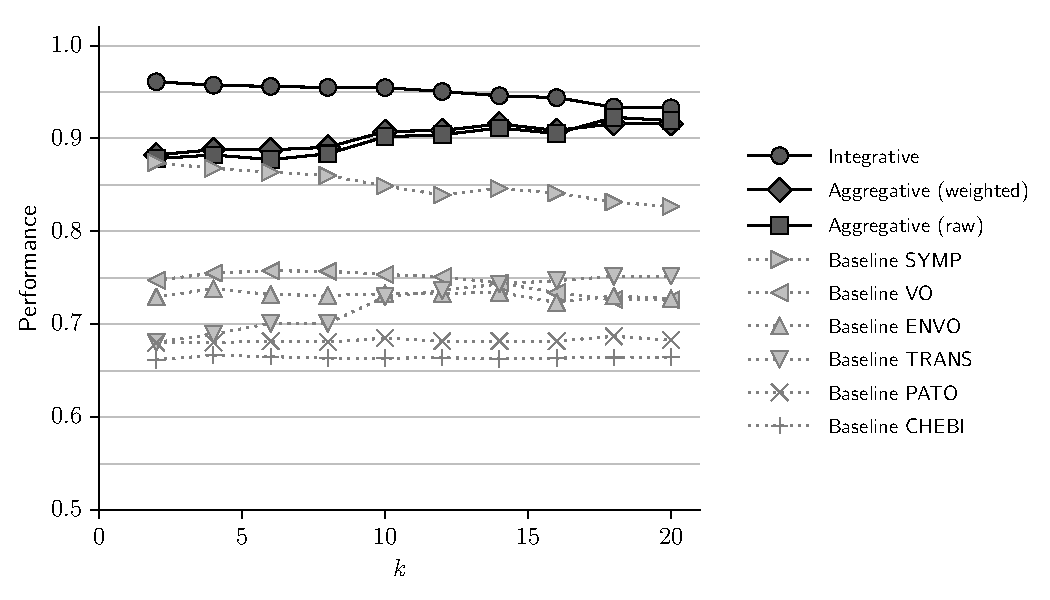
\includegraphics[width=0.9\linewidth]{images/epidemic-purge-resnik.pdf}
    \caption[Semantic similarity in the purged Epidemic Marketplace dataset]{These results show the performance of the semantic similarity measures using the various settings detailed in the beginning of this section. This graph was obtained using the purged dataset, \ie excluding \ontology{MeSH} and \ontology{NCIt} annotations. Baseline settings are presented as dotted grey lines, and the multi-domain settings as black solid lines.}
    \label{fig:epiwork-purge}
\end{figure}

\begin{figure}
    \centering
     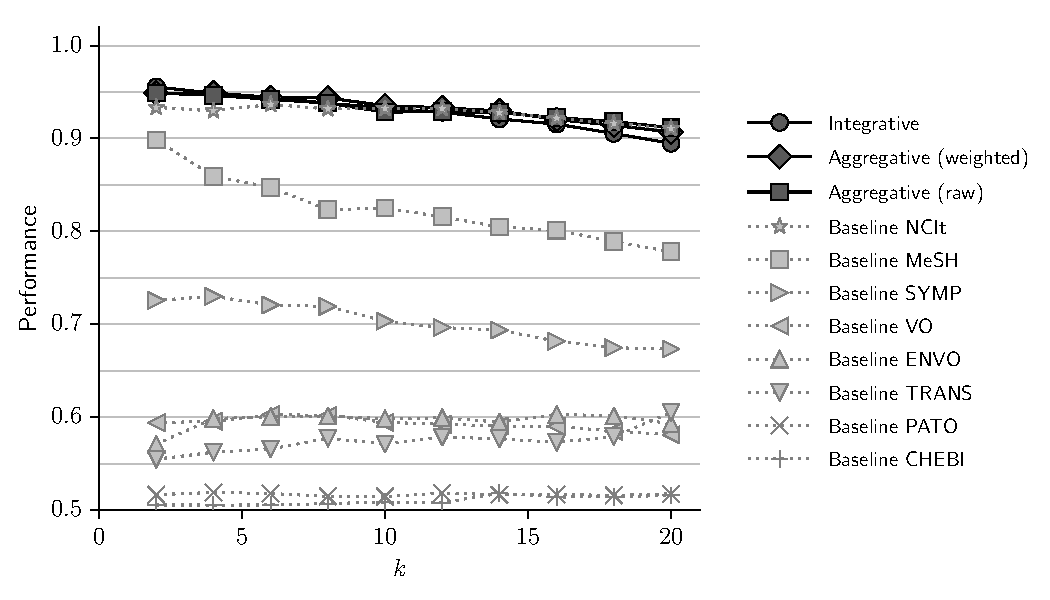
\includegraphics[width=0.9\linewidth]{images/epidemic-regular-resnik.pdf}
    \caption[Semantic similarity in the raw Epidemic Marketplace dataset]{These results show the performance using the various settings detailed in the beginning of this section. This graph was obtained using all annotations, including \ontology{MeSH} and \ontology{NCIt}. Baseline settings are presented as dotted grey lines, and the multi-domain settings as black solid lines.}
    \label{fig:epiwork}
\end{figure}

The graph presented in \figref{fig:epiwork-purge} depicts this evaluation measure with respect to the several similarity settings defined in this section, using various values of~$k$ in the ML-KNN algorithm. As can be seen, the integrative approach always outperforms the other settings, independently of the value of~$k$, thus showing the superiority of multi-domain semantic similarity in this dataset over single-ontology measures. We can observe that the single-ontology measure performed on the \ontology{SYMP} baseline (using the symptoms ontology) is the most successful baseline. This is justified by considering the annotation profile shown in \tabref{tab:epiwork-purge}. In fact, except for \ontology{DOID}, this is the domain with the highest coverage and the highest volume of annotation.

Additionally, from the set of domains used to annotate these resources, symptoms are the most closely related to diseases. This baseline shows a performance comparable to the \textbf{Aggregative} approaches, especially for low values of~$k$, which means that the other domains have little to add to the information already provided by \ontology{SYMP} (the gap increases with the increase of~$k$). However, the \textbf{Integrative} approach shows a higher performance than the other multi-domain approaches for all values of~$k$. This may be justified with the fact that many resources are annotated with different sets of domains. For example, consider the calculation of similarity between a resource that has annotations from \ontology{TRANS} with a resource with \ontology{TRANS}, \ontology{SYMP} and \ontology{VO} annotations. In the \textbf{Aggregative} approaches, only the \ontology{TRANS} domain can be used, which results in the method ignoring some annotations; but the \textbf{Integrative} approach uses all annotations, irrespective of domain, thus being able to more correctly discern between the resources and being, in general, more accurate. This appears to be an especially relevant result in this dataset, as the coverage of the various domains is small.
\looseness=1

% On the one hand, we need to consider the ``noise'' introduced into the multi-domain measure by the other ontologies. For example, similarity measured in the \ontology{TRANS} domain performs poorly, even though it is used to annotate a significant fraction of the resources ($60.6\%$). However, only $9$~distinct concepts are used for this domain, which means that its discriminating power is severely affected when compared, for instance, to the \ontology{VO} domain (lower coverage but higher diversity). Thus, introducing these annotations into the multi-domain measure does not increase the performance significantly.

\figref{fig:epiwork} contains an equivalent graph, obtained in the regular dataset (including \ontology{MeSH} and \ontology{NCIt} annotations). Notice that the baseline performances are not the same as in the previous purged dataset, because this raw dataset contains more resources, specifically more resources that do not have annotations in the domains of those baselines, decreasing their performance. The main conclusion that can be taken from this result is that similarity calculated with multi-domain approaches performs as well as the best baseline (calculated with the \ontology{NCIt} domain). On the one hand, this domain corresponds to the maximum coverage, volume and diversity (see \tabref{tab:epiwork-summary}), and as such the rest of the domains have little information to add to it. On the other hand, these other domains manage to avoid adding noise to the multi-domain measures: multi-domain measures never show a performance significantly lower than the \ontology{NCIt} baseline. As expected, the best baselines correspond to the two ontologies that span all the domains of annotation.
\looseness=1


\subsection{Metabolic Pathways Dataset} \label{sub:results/pathways}

KEGG pathways are manually classified into $33$~distinct groups. For example, ``Lysine degradation'' is classified into the ``Amino acid metabolism'' group, since Lysine is an amino acid. I exploited this classification in evaluating the performance of semantic similarity in the metabolic pathways dataset by using the similarity values to predict that same manual classification. As above, this is a strategy that belongs to the ``Classification prediction for single entities'' branch of the validation hierarchy. Specifically, I applied the machine-learning algorithm $k$-nearest neighbours (\knn) to predict the class of each pathway given its similarity with the other pathways. The algorithm can be approximately described as follows:
\begin{enumerate}
    \item For each pathway~$p$, compare it to all other pathways using semantic similarity, and find the $k$~pathways most similar to it. Call this group of neighbour pathways $Q_p = \{q_1, \dots, q_k\}$.
    \item Find the class of each of these neighbours, $C(q_i)$ for~$i=1,\ldots, k$.
    \item For each class~$c'$ among all the $33$~above, count the number of neighbour pathways in~$Q_p$ that are part of that class: $f(c') = |\{q_i \in Q_p \mid C(q_i) = c'\}|$.
    \item Select~$c = \argmax_{c'}f(c')$, \ie the most common class among the $k$~neighbours. In case of a tie, the selected class is the one with a higher sum of the similarities between $p$ and the pathways in that class.
    \item Each pathway is then classified as ``correct'' if the selected class corresponds to the real one, and ``incorrect'' otherwise.
    \item Performance is reported as the fraction of correct pathways.
\end{enumerate}

As can be seen from \figref{fig:pathways}, performance was calculated for various values of~$k$, and in almost all cases we observe that multi-domain settings outperform single-ontology ones.

A conclusion that can be taken from this figure is that the different domains perform differently from one another, with the ``\ontology{GO} terms'' baseline performing on par with the \textbf{Aggregative(raw)} multi-domain setting. I refer the reader again to \tabref{tab:pathways-summary} (page~\pageref{tab:biomodels-summary}), which summarises the annotations in each domain. For example, only~$42.4\%$ of the pathways contain information on drugs, which means that only about~$18\%$ of all the pairs of pathways can use this information. Thus, using this domain results in low performance, as expected. On the other hand, all pathways are annotated with \ontology{GO} concepts, with a volume of about $30$~concepts per pathway. This, coupled with the fact that semantic similarity in the biomedical domain has been initially explored in \ontology{GO} and has been since thoroughly studied in this ontology more than in the other ontologies, means that it is not surprising that there is little improvement when going from the \ontology{GO} baseline to the multi-domain approaches. Nonetheless, improvements are observed in multi-domain settings for most values of~$k$.

\begin{figure}
    \centering
    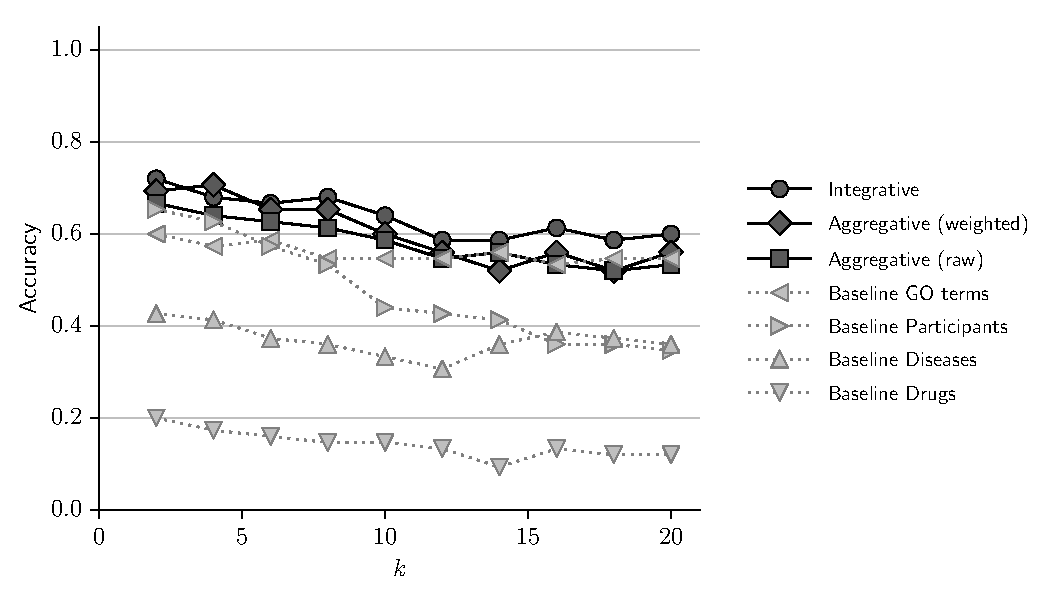
\includegraphics[width=0.9\linewidth]{images/pathways-resnik.pdf}
    \caption[Semantic similarity in the Metabolic Pathways dataset]{These results show the fraction of pathways correctly classified, using the various settings detailed in the beginning of this section. Baseline settings are presented as dotted grey lines, and the multi-domain settings as black solid lines.}
    \label{fig:pathways}
\end{figure}

\begin{figure}
    \centering
    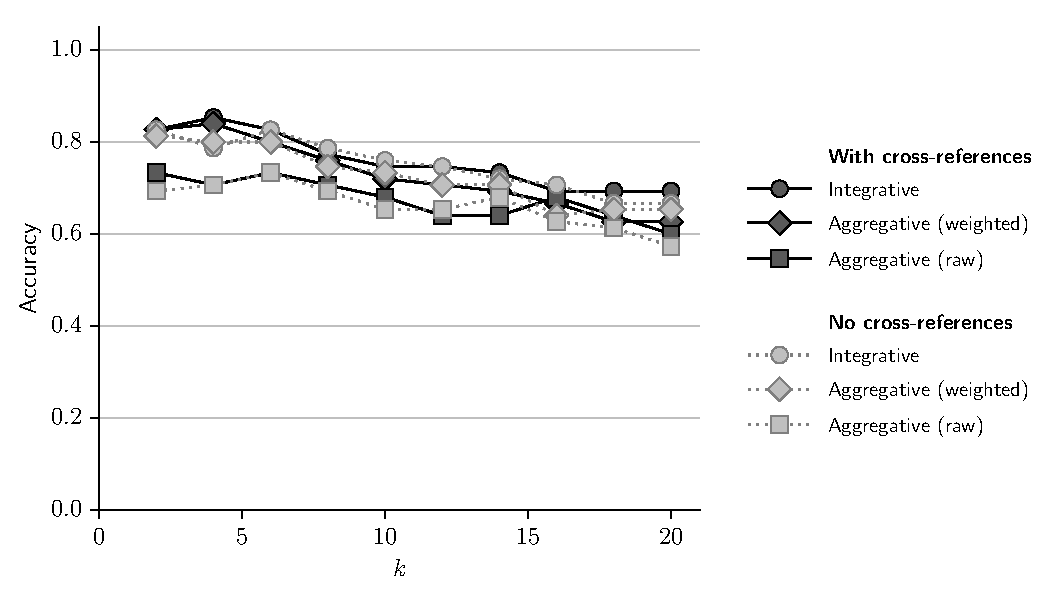
\includegraphics[width=0.9\linewidth]{images/pathways-ferreira-xref-noxref.pdf}
    \caption[Effect of cross-references on the performance of semantic similarity]{As before, these results show the fraction of pathways correctly classified, but now using only the multi-domain approaches. The black solid lines show the results obtained using the cross-references that connect the \ontology{GO} and \ontology{CHEBI} ontologies; the dotted grey lines represent the results obtained without those cross-references. Only the $\ferreira$ measure can make actual use of the cross-references, and as such this graph shows the results obtained with that measure.}
    \label{fig:xref-pathways}
\end{figure}

Unlike what happens in the previous dataset, the \textbf{Integrative} setting does not clearly outperform the other multi-domain measures. I justify this observation with the fact that the domains in this dataset are more well-balanced than in the previous one, since a majority of the pathways are annotated in a significant portion of the domains ($70\%$~of the pathways have annotations in $3$ or~$4$ domains). The ``Participants'' baseline also shows a high accuracy: it was already established that semantic similarity is a useful technique in \ontology{CHEBI}~\citep{Ferreira2010,Ferreira2013}. While the accuracy for the ``Metabolites'' and the ``Drug'' baselines is low, coupling this information with the other domains increases the performance with respect to the best baseline, namely in the \textbf{Aggregative(weighted)} and \textbf{Integrative} approaches.

In cases like these, where the domains are balanced in terms of number of annotations, and are known to produce good results with semantic similarity, I anticipate that there is no way, short of actually evaluating the results of semantic similarity, to determine which of the multi-domain approaches will lead to the best performance. Even so, I expect that at least the integrative approach will always outperform the best single-ontology baseline.

\begin{figure}
    \centering
    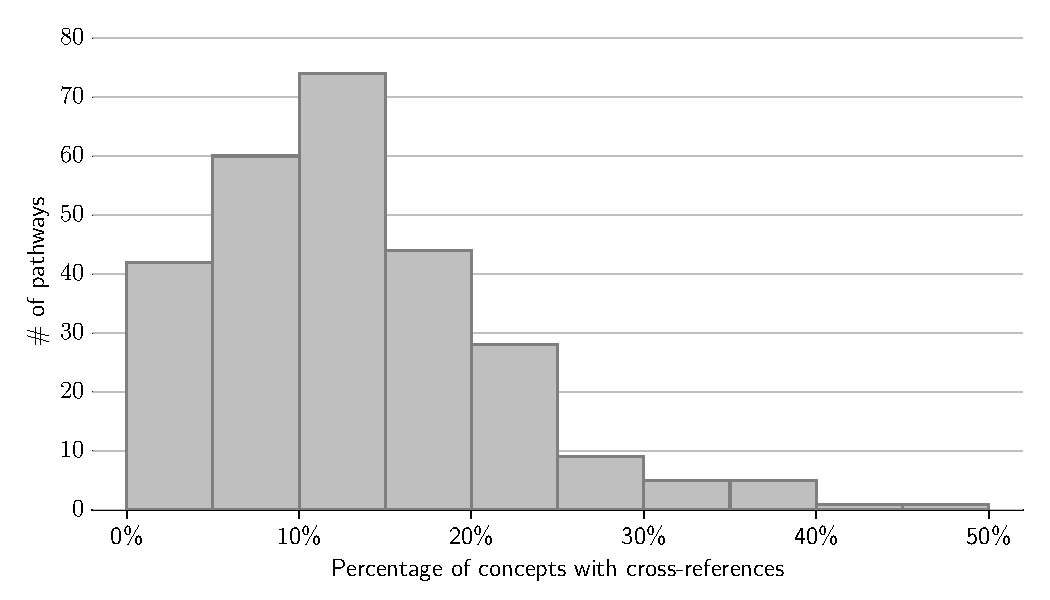
\includegraphics[width=0.9\linewidth]{images/pathways-xref-histogram.pdf}
    \caption[The distribution of the percentage of annotations that have cross-references]{This histogram plots the amount of pathways, among the $269$ in the Metabolic Pathways dataset, according to how many of their annotations have inter-ontology cross-references.}
    \label{fig:xref-histogram}
\end{figure}

As hinted before, it is also relevant to study the effect that multi-domain cross-references have on semantic similarity. Since $\sim[Resnik]$ is agnostic to cross-references, I used instead my own measure of relatedness,~$\ferreira$ (\secref{sec:enhancements/relatedness}). Given that using the links between ontologies means that the semantic relatedness algorithm has more information to work with, I originally expected that measures using cross-references would have a higher performance. \figref{fig:xref-pathways} shows the reverse: adding cross-references to the store of information accessible to the algorithm has no significant impact on the performance. The main reason for this result seems to be that the amount of cross-references is still low, when compared to the size of the dataset and the size of the ontologies. For example, cross-references exist only in \ontology{GO} ontology, and only for $25\%$~of its concepts (corresponding to only approximately~$11\%$ of the concepts of all domains). \figref{fig:xref-histogram} shows that in the majority of pathways, only~$15\%$ of the annotations have disjointness information.

On the other hand, this relatedness algorithm has been validated in \ontology{FMA} measures, which may also contribute to it not being able to use the information from \ontology{GO} cross-references. In fact, while $\ferreira$ outperforms $\sim[Resnik]$ by a large amount (\cf the results in \figref{fig:pathways} and \figref{fig:xref-pathways}, where we can see that the \textbf{Integrative} approach has accuracy values ranging in the interval~$(0.6, 0.7)$ for $\sim[Resnik]$ and in the interval~$(0.7, 0.8)$ for $\ferreira$), it seems to be unable to use the cross-references to improve its results even further.


\subsection{Biochemical Models Dataset} \label{sub:results/biomodels}

To evaluate semantic similarity in this dataset, I asked a Systems Biologist (Dr Bernard de Bono from University London College) to evaluate a predetermined set of $250$~pairs of biomodels, each according to how similar the two biomodels in the pair are (see \secref{sec:data/biomodels} and \figref{fig:biomd}).

To assess the performance of each semantic similarity measure, I evaluated the degree to which the measures reflect the manual similarity values, an approach that is classified, according to the hierarchy in \figref{fig:hierarchy}, as a ``Correlation with a manual anchor measure''. Since the gold-standard values are not continuous but rather ordinal, this correlation cannot be measured with Pearson's correlation coefficient, but should instead be measured with non-parametric coefficients such as Spearman's rank coefficient or Kendall's~$\tau$ coefficient. The results shown in this section correspond to Spearman's rank coefficient, but the ones obtained with Kendall's coefficient are equivalent in all aspects.

As can be seen from \figref{fig:biomodels}, the integrative approach outperforms all the other settings, namely the single-ontology ones. In this case, it is even more interesting to compare the results obtained with $\sim[Resnik]$ \vs $\ferreira$ (see \figref{fig:biomodels-ferreira}). The most noticeable difference is that the \textbf{Integrative} approach achieves a much higher performance with $\ferreira$ than with $\sim[Resnik]$, even though the single-ontology baselines and the aggregative approaches do not exhibit as large an increase. This seems to indicate that this multi-domain approach is able to thoroughly explore the multidisciplinarity with this measure in a way that it cannot with $\sim[Resnik]$.

\begin{figure}
    \centering
    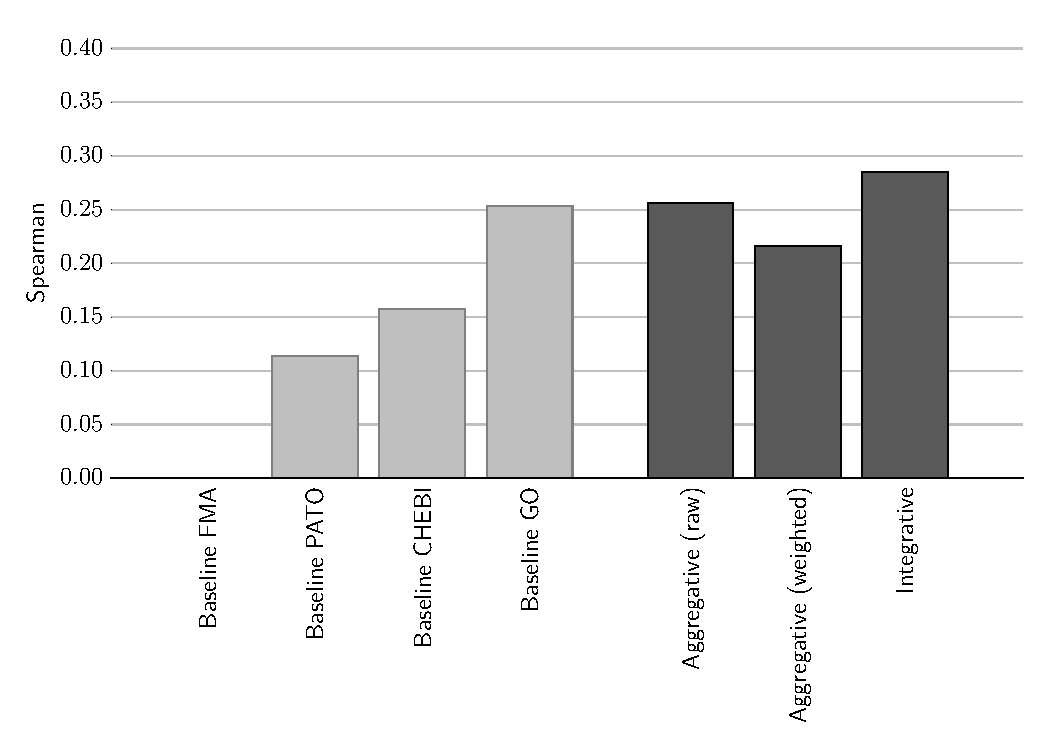
\includegraphics[width=0.9\linewidth]{images/biomodels-resnik.pdf}
    \caption[Semantic similarity in the Biochemical Models dataset with~{\boldmath$\protect\sim[Resnik]$}]{These results show the Spearman's rank coefficient between each semantic similarity measure and the gold-standard, measured with $\sim[Resnik]$. In general, the multi-domain measures (shaded in a darker tone of grey) outperform the single-ontology ones (shaded in a lighter tone of grey).}
    \label{fig:biomodels}
\end{figure}

Like in the previous dataset, \ontology{GO}-based semantic similarity performs highly (even higher than the \textbf{Aggregative} approaches). I argue that this happens for the same reasons: semantic similarity has been studied to a higher degree of detail in \ontology{GO} than in the other ontologies, and the coverage and volume of \ontology{GO} annotations is higher than the rest of the domains. In particular, semantic similarity in \ontology{FMA} yields a performance of $0$~because, even though $11$~models contain \ontology{FMA} annotations (see \tabref{tab:biomodels-summary}, the gold standard never pairs one of these $11$~models with another one of them.

Like in the first dataset, there is a discrepancy between the three multi-domain settings, as the integrative approach outperforms the \textbf{Aggregative} ones. I believe the reasons for this are equivalent to the ones presented before: in the \textbf{Aggregative} approach, the final similarity score will be an average of four measures, three of which exhibit a low performance. It is not surprising, therefore, that its performance does not increase much with respect to the ``\ontology{GO}'' baseline (in fact, performance decreases for the \textbf{Aggregative (weight)} approach with $\sim[Resnik]$).

Again in this dataset, it can be observed that using cross-references does not produce any significant difference. In this case, in fact, I do not present a new figure as it would be so similar to the ones already presented that only a reader willing to use a ruler would be able to tell the difference in the height of the bars. The differences are instead presented in \tabref{tab:epiwork-xref}.

\thisfloatontop
\begin{figure}
    \centering
    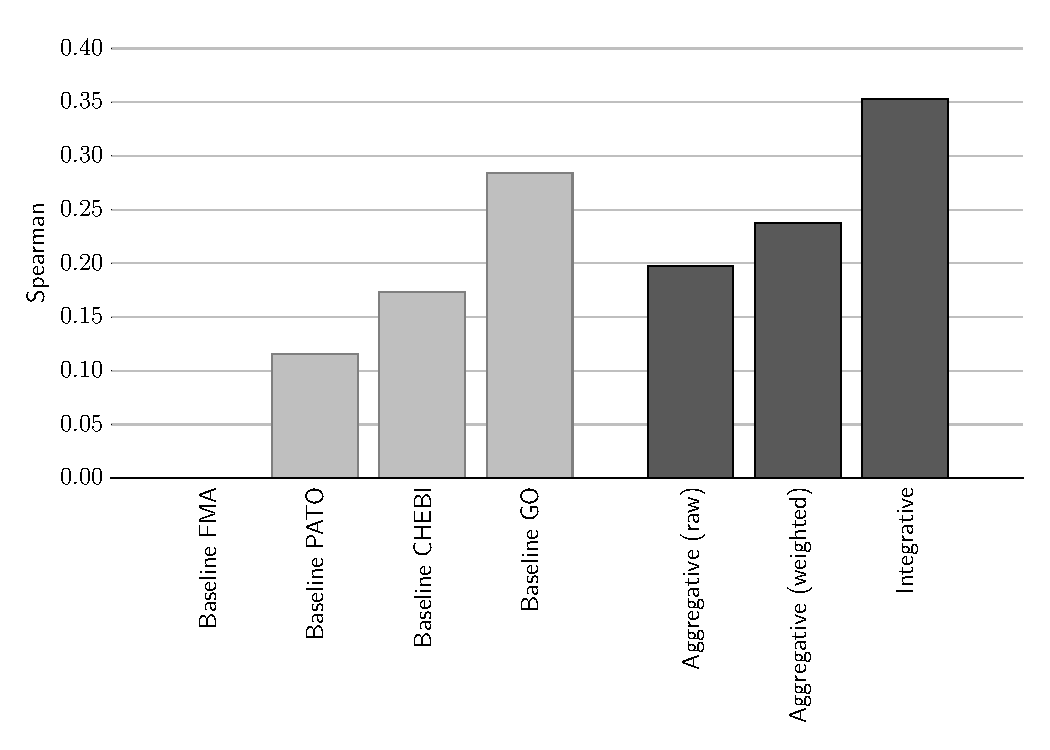
\includegraphics[width=0.9\linewidth]{images/biomodels-ferreira.pdf}
    \caption[Semantic similarity in the Biochemical Models dataset with~\boldmath$\ferreira$]{These results show the Spearman's rank coefficient between each semantic similarity measure and the gold-standard, measured with $\ferreira$ relatedness measure instead of $\sim[Resnik]$. In general, the multi-domain measures (shaded in a darker tone of grey) outperform the single-ontology ones (shaded in a lighter tone of grey).}
    \label{fig:biomodels-ferreira}
\end{figure}

One other aspect to consider in this case is the overall low correlation coefficient obtained with any of the measures and the multi-domain approaches. The best performance in all cases is obtained with $\ferreira$ with the \textbf{Integrative} approach, but this corresponds only to a correlation of~$0.352780$. Although not entirely statistically significant, I also calculated Pearson's correlation coefficient for these results, and obtained a value of~$0.581401$ for this case. A work by \citet{Hauke2011} shows that when Pearson's correlation coefficient is higher than Spearman's, then there is a (weak, at least) linear correlation between the two variables being measured (as opposed to other types of correlation): in this case, semantic similarity with the $\ferreira$ measure using the \textbf{Integrative} multi-domain approach, and the manual similarity values assigned by the Systems Biology expert. But a linear correlation with Pearson's coefficient of~$0.581401$ is still a low value. As such, the proposed measures seem to still be lacking in some way, as they do not properly reflect the expert assessment of similarity.

Fortunately, this result does not interfere with my hypothesis. The results presented in the figures of this section can still be used to show that multi-domain measures outperform single-ontology ones.

\begin{table}
\caption[Effect of cross-references on the performance of semantic similarity in the Biochemical Models dataset]{These results show the Spearman's rank coefficient between semantic similarity and the gold-standard, measured with $\ferreira$ relatedness measure. Each column reflects the results obtained without and with cross-references.}
\label{tab:epiwork-xref}
\centering
\small
\begin{tabular}{llcc}
\toprule
\multicolumn{2}{l}{\textbf{Measure}} & \textbf{No cross-references} & \textbf{With cross-references} \\
\midrule
Baseline    & \ontology{FMA}               & 0.000000 & 0.000000 \\
            & \ontology{PATO}              & 0.115841 & 0.115841 \\
            & \ontology{CHEBI}             & 0.173646 & 0.173358 \\
            & \ontology{GO}                & 0.283925 & 0.286247 \\
\addlinespace
\multicolumn{2}{l}{Aggregative (raw)}      & 0.197591 & 0.196394 \\
\multicolumn{2}{l}{Aggregative (weighted)} & 0.237164 & 0.239875 \\
\multicolumn{2}{l}{Integrative}            & 0.352780 & 0.359541 \\
\bottomrule
\end{tabular}
\end{table}

\chapter{Semantic similarity software suite} \label{chap:technical}

Working with Web Ontology language (OWL) files is not easy, especially when doing many small things a large number of times. Algorithms that depend on ontology information, such as semantic similarity, cannot be expected to load a set of potentially very large OWL files just to find specific facts represented therein, like what the superclasses of a given class are.

To satisfy the requirements of such algorithms, I propose a solution that enables programmatic access to the information contained in an ontology that does not depend on reading and parsing the ontology for every set of requests, but instead provides \emph{random access} to the elements of the ontology, including not only the concepts but also the axioms stated between them. The main idea of this solution is to insert \emph{useful} information from the OWL files into an SQL database, which can then be queried by semantic similarity algorithms. This software is called \owlsql.

Apart from this storage mechanism, I also produced and released a piece of software responsible for computing semantic similarity between concepts and annotated entities in a manner that
\begin{paralist}
    \item depends on the information stored by \owlsql, and
    \item uses a flexible model that can be quickly used by any developer to add their own semantic similarity algorithms.
\end{paralist}
This is called the Multi-Ontology Semantic Similarity (\mossy) tool.


\section{\owlsql} \label{sec:technical/owlsql}

\begin{note-paper}
    \owlsql's source code is available at \url{https://github.com/jotomicron/OWLtoSQL}.
\end{note-paper}

Biomedical ontologies are distancing themselves from the simple ``hierarchy of concepts'' model and are becoming increasingly more complex. As we saw in the previous chapters, ontologies contain disjointness information, existential quantifications, and even other types of axioms. For example, \ontology{FMA} contains the axiom
\begin{axiom}
    \existential{Heart}{has-part}{Aortic valve}
\end{axiom}
which means that for each \term{Heart}, there is some \term{Aortic valve} to which the heart is related by means of the property~\prop{has-part}; in less technical jargon, this means that all hearts have one aortic valve. Properties themselves are also related to each other, \eg \prop{negatively-regulates}, a property of \ontology{GO} that relates proteins with the processes that they inhibit, is a sub-property of \prop{regulates}.

On the one hand, this increased expressiveness leads to an increase in the richness of the information that can be represented in an ontology, ultimately allowing for a more faithful representation of the reality in a machine-understandable manner. On the other hand, this richness implies a certain complexity in the parsers of the language and an increased difficulty in extracting information from an OWL file in a \emph{random access} way. For example, finding the parts of the \term{Heart}, as represented in \ontology{FMA}, is a two-step task:
\begin{enumerate}
    \item \label{item:load-subtask} open and parse the \nolinkurl{fma.owl} file into RAM-accessible data structures; and
    \item query the data-structures for the necessary information.
\end{enumerate}

Several APIs (Application Programming Interfaces) have been created to perform these steps, such as Jena~\citep{Carroll2004} and OWL-API~\citep{Horridge2011}. Once opened, the extraction of information is mostly as a small sequence of look-up operations in RAM accessible hashmaps. However, for the one-time random access to the information, this solution is not suitable, as step~\ref{item:load-subtask} is time consuming and does not scale with the size of the ontology (to open and parse the aforementioned \nolinkurl{fma.owl} file, a regular-size personal desktop computer \mdash four 2GHz~CPUs and 4GB of RAM \mdash takes up to $30$~seconds). Having such a large waiting time for one semantic similarity request is highly undesirable: \eg a web service that computes semantic similarity between annotated entities and that takes $30$~seconds to return the similarity between \term{Heart} and \term{Trachea} will likely fail to be adopted by the community.

In order to solve this problem, there are two different possible avenues.

The first approach is to open the OWL file within a computer process capable of inter-process communication, which can then answer client questions like the one about the branches of the \term{Trachea}. This approach is quite flexible, since, given an appropriate protocol for the communication between server and clients, it allows the query of any OWL question. However, it is difficult to implement: the communication protocol between the processes needs to align with the OWL specification to ensure that all OWL-valid constructions can be queried and answered. While promising, this idea has yet failed to deliver fully functional software: the only existing implementation I know is OWLlink~\citep{Liebig2009}, which is still lacking some useful features. For example, it does not support asking for the names of the concepts, and it is not fully aligned with the latest OWL specification. Additionally, development has been stalled since August 2011.

The second approach is to open the OWL files and extract its information into a more accessible medium, such as a database. OWL can be fully serialised in RDF (see \secref{sec:concepts/semantic-web}), and as such RDF triple stores are an intuitive candidate for storing the OWL ontology, such as OpenRDF Sesame, Jena and OpenLink Virtuoso. These programs are, however, more suited for dealing with contexts where the ontology information is used to reason about the existing data, \eg to infer the type of some instances based on the properties asserted about those instance; instead, my work in semantic similarity is mostly related to querying the ontology itself: examples of question that are in realm of semantic similarity include ``what things are part of a \term{Heart}?''\ and ``what are the superclasses of \term{Aortic valve}?''. Additionally, querying over triple stores is usually done with SPARQL queries~\citep{Harris2013}, which is an OWL-agnostic language. While efforts have been made in order to introduce OWL-aware query languages, such as SPARQL-DL~\citep{Sirin2007} and SQWRL~\citep{OConnor2009}, they have not been implemented in any of the existing triple stores.

% As such, converting OWL requests into SPARQL queries requires an intimate knowledge of the RDF serialization of OWL: to query for the classes that are part of the ``Heart'' (\ie to find all \term{?x} such that \existential{Heart}{has-part}{?x}), one would need to use this corresponding SPARQL query:

% \begin{minted}{sparql}
% PREFIX rdfs: ???
% PREFIX owl: ???
% PREFIX fma: ???
% SELECT ?x WHERE {
%    fma:Heart rdfs:subClassOf ?y .
%    ?y a owl:Restriction ;
%       owl:onProperty fma:has-part ;
%       owl:someValuesFrom ?x .
% }\end{minted}

Furthermore, even a fully working triple store solution equipped with an OWL-aware query language can be slower than necessary for some user needs. For example, asking for all the leaf concepts (concepts which have no subclass of their own) may be a time consuming task, since it involves querying, for each concept, if it has any subclasses. While reasoners can alleviate this task by allowing certain queries to be performed faster (\eg reasoners build a static hierarchy that allows a quick answer to queries like ``Is $A$ a subclass of~$B$?''), some queries may still take a long time to run. In fact, a reasoner does not give the number of hypernymy relationships between two concepts, but only whether such a path exists. As such, it can be argued that some algorithms would benefit from a type of caching that computes a single time and stores the information they need in an easy-to-use, fast, and random-access back-end, which is not yet available.

In this context, it is relevant to introduce the idea of \emph{useful} information: presumably, an information-intensive algorithm such as semantic similarity has a static set of information requirements, an \emph{a-priori} established set of axiom types that are needed for the algorithm to work. For example, some semantic similarity algorithms need to know the superclasses of a given class and ``how far'' the superclass is to the class itself in the hierarchy. As such, and for the purpose of this discussion, I define \emph{useful} information as the total information that an algorithm needs to extract from the ontology in order to run without parsing the original OWL file and without performing time- and resource-consuming computations.

Based on this idea, I developed \owlsql, an extensible Java program that is responsible for reading OWL files using the OWL-API and saving any useful information into an underlying relational MySQL database. This allows random-access to any information that is encoded in the original ontology without the need to parse the ontology file again. Indices created on the stored tables guarantee fast retrieval of this information.

This is not the first time that a proposal like this has been made. \citet{Zhou2006} and \citet{Henss2009} proposed two previous solutions that tried to map all the OWL specification into a back-end database. These solutions, however, are buggy (I have in fact personally approached one of these authors requesting assistance with a bug I experienced, but their response was that they knew about the bug I was seeing, that it was due to a third party library, and that they could not offer further help), outdated (development has been stalled at least since 2010) and do not allow the insertion of non-standard information in the database (such as the edge distance in the class-subclass hierarchy). As such, I had to roll out my own solution.

Other papers have explored the idea of using OWL to build SQL databases, but they use OWL as a means to develop the database \emph{schema}, not to populate a database with the information encoded in the ontology \citep[\eg][]{Astrova2007,Zina2014}.


\subsection{The software model} \label{sub:owlsql/model}

From the point of view of its user, the interface of \owlsql\ is a configuration file that provides:
\begin{itemize}
    \item the settings needed to connect to the MySQL database;
    \item the list of ontologies that are to be loaded in memory and whose information is to be stored in the database; and
    \item a list of \emph{extractors}, which are Java classes that are responsible for extracting the information from the memory-accessible data-structures containing the ontologies and putting that information in the database.
\end{itemize}

\owlsql\ then
\begin{paralist}
    \item opens a connection to the MySQL server,
    \item loads the ontologies using OWL-API, and
    \item \emph{blindly} executes the code of each specified extractor.
\end{paralist}
Each extractor is an implementation of the abstract Java class \texttt{Extractor}, which provides convenience methods to access the MySQL database and the configuration options. In this manner, the definition of \emph{useful} information is provided by the user as the set of extractors to run (see \figref{fig:model}).

Importantly to the idea behind \owlsql\ is the notion that it is highly extensible. Anyone with knowledge of Java and the OWL-API can create their own Java class that extends \texttt{Extractor} and then use it as a \emph{plugin} to \owlsql.

\begin{figure}
    \centering
    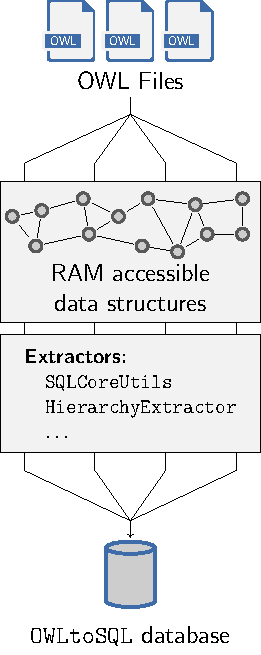
\includegraphics{images/owlsql.pdf}
    \caption[Operation model of \owlsql]{Several OWL files can be used by this software, which opens and parses them into memory-accessible data-structures (usually hashmaps that allow quick data lookup). Several Java classes extending a common interface named \texttt{Extractor} are then used to extract information from these data-structures and store it in the underlying database.}
    \label{fig:model}
\end{figure}


\subsection{Configuration file} \label{sub:owlsql/config}

\owlsql\ reads from a configuration file that the user is responsible for generating, which enables the user to choose the ontologies to load and extractors to run. The configuration file is written using JSON format and it must contain the following elements:
\begin{itemize}
    \item \json{mysql} determines the host, database name, user name and password needed to connect to the SQL server.
    
    \item \json{ontologies} is a list of strings, each containing the \texttt{url} that determines where the ontology should be loaded from. These options expect valid URLs that can be used by the OWL-API: as such, URL schemas such as \texttt{file:} or \texttt{http:} are supported.
    
    \item \json{extractors} contains a list of extractor specifications. These are themselves JSON objects containing a \json{class} element that points to the binary name of an extractor Java class and any additional elements that are used to tune the extractor's behaviour. In the case illustrated in \lstref{lst:owlsql-config}, the parameter \json{properties} contains the standard label property defined by the W3C committee~\citep{Guha2014}. Interpreting these options is the responsibility of the extractor class.
\end{itemize}

\begin{listing}
\centering
\begin{minted}{json}
{
    "ontologies": [
        "http://purl.obolibrary.org/obo/go.owl"
    ],
    "mysql": {
        "hostname": "localhost",
        "database": "db_name",
        "username": "user",
        "password": "passwd"
    },
    "extractors": [
        {
            "class": "pt.owlsql.extractors.NamesExtractor",
            "properties": [
                "http://www.w3.org/2000/01/rdf-schema#label"
            ]
        },
        {
            "class": "pt.owlsql.extractors.HierarchyExtractor",
        },
        {
            "class": "pt.owlsql.extractors.LeavesExtractor",
        }
    ]
}
\end{minted}
\caption[A possible \owlsql\ configuration file]{These examples shows the configuration that needs to be provided to \owlsql\ in order to store the information represented in the Gene Ontology, and specifies that the information to extract is the labels of the concepts, the class-subclass hierarchy and the set of leaf concepts.}
\label{lst:owlsql-config}
\end{listing}

More than one extractor can be given (as exemplified in \lstref{lst:owlsql-config}), and the order in which they are given in the configuration file is the order in which they are executed by \owlsql.


\subsection{Built-in extractors} \label{sub:owlsql/builtin}

Even though \owlsql\ provides the possibility for user-defined extractors, it provides a significant number of built-in extractors. I mention five of them, as an illustration.

The most important one, which is fundamental for the proper functioning of this software, is named \texttt{SQLCoreUtils} and it is responsible for extracting the bare minimum information from the OWL files: the entities represented in each loaded ontology. Each entity is stored in a master table and a unique integer identifier is provided to it. This identifier is more suitable for database management than the actual Internationalized Resource Identifier (IRI) (see \secref{sec:concepts/owl}) that ontologies provide, as integers can be more easily indexed than the IRI of the entities, which are text that is, in principle, not bounded by a maximum length. The table saves the identifier, the IRI of the entity, and the type of OWL entity that it represents. For example, if an ontology makes use of the concept \nolinkurl{http://www.w3.org/2002/07/owl\#Thing}, this entity is stored in the database as an \texttt{OWLClass} associated with that IRI, and a unique integer identifier is assigned to it.

\texttt{HierarchyExtractor} builds and stores the full class-subclass hierarchy of the loaded ontologies. Take for instance the small ontology illustrated in \figref{fig:small-ontology}; this extractor stores in the database the facts ``\term{Wolf} \prop{is-a} \term{Mammal}'' and ``\term{Cow} \prop{is-a} \term{Mammal}'', which are direct class-subclass relationships, but also facts like ``\term{Wolf} \prop{is-an} \term{Animal}'', which can only be obtained by traversing two relationships. As such, along with each fact, this extractor stores the minimum distance between the two classes.

\begin{figure}
    \centering
    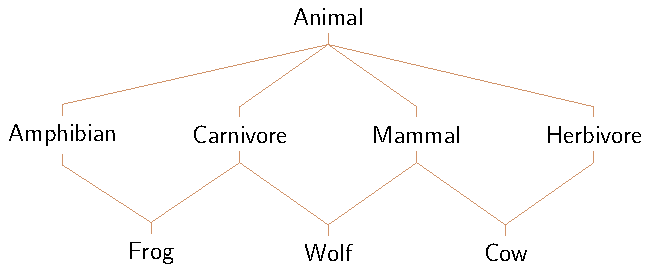
\includegraphics{images/animal-ontology.pdf}
    \caption[A toy ontology representing some animals]{The classes are organised in a class-subclass hierarchy, where the maximum distance between any concept and the root is $2$.}
    \label{fig:small-ontology}
\end{figure}

\texttt{LeavesExtractor} creates a table that contains the leaves of the ontologies, \ie the classes that have no subclass. This extractor depends on the information stored by the previous one, and as such must always be executed after the previous one.

\texttt{ICExtractor} calculates the information content of each concept (see \secref{sec:sota/node}, specifically \eqref{eq:resnik-ic,eq:seco}). Four different algorithms are calculated and stored in the database.

\texttt{NamesExtractor} stores the names of the concepts of the ontologies in the database. By default, this extractor uses the property \prop{rdfs:label} to find the names of entities, but it is possible to specify a different property in the configuration file (see~\lstref{lst:owlsql-config}).


\subsection{Retrieval from the database} \label{sub:owlsql/retrieval}

The retrieval of information from the database is done directly from the database. This requires that the users of the \owlsql\ back-end are familiar with how the information is stored in the database.

While there are some disadvantages to this (the information is stored in a non-standard format), proper documentation can mitigate these aspects. On the other hand, this allows any programming language that has a MySQL driver to access the information.

% For example, the \texttt{SQLCoreUtils} includes the following methods:
% \begin{itemize}
%   \item \texttt{getAllEntities()}: retrieves a set containing all the OWL entities stored in the database
  
%   \item \texttt{getDefiningOntologies()}: retrieves the \texttt{OWLOntologyID} of the ontologies that make use of a given OWL entity
  
%   \item \texttt{getEntity(int)}: retrieves the OWL entity that corresponds to the given internal ID. This method is essential for applications that need to retrieve information from the database, since the information is stored in terms of the internal Identifiers, but applications want the actual OWL entities.
  
%   \item \texttt{getID(OWLEntity)}: this is the reverse of the previous method; it returns the internal ID of a given OWL entity.
% \end{itemize}

% These methods are extensively used by the other extractors, particularly the \texttt{getID()} method. For example, \lstref{lst:hierarchy-snippet} shows a snippet of the extracting method of \texttt{HierarchyExtractor}. It uses the method \texttt{SQLCoreUtils.getID()} to convert the OWL classes into internal unique identifiers that are then inserted into the table (see lines~1, 15 and~16).

% \begin{listing}
% \centering
% \begin{minted}[gobble=4]{java}
%     SQLCoreUtils utils = getDependency(SQLCoreUtils.class);
    
%     PreparedStatement insertStatement = getConnection().prepareStatement(
%         "INSERT INTO hierarchy (subclass, superclass, distance) " +
%         "VALUES (?, ?, ?)");
    
%     insertStatement.setInt(3, 1); // Distance is 1 for direct class-subclass
%     for (OWLSubClassOfAxiom ax : ontology.getAxioms(AxiomType.SUBCLASS_OF)) {
%         OWLClassExpression subClass = ax.getSubClass();
%         OWLClassExpression superClass = ax.getSuperClass();
    
%         if (subClass.isAnonymous() || superClass.isAnonymous())
%             continue;
    
%         int subClassID = utils.getID(subClass.asOWLClass());
%         int superClassID = utils.getID(superClass.asOWLClass());
    
%         insertStatement.setInt(1, subClassID);
%         insertStatement.setInt(2, superClassID);
%         insertStatement.execute();
%     }
% \end{minted}
% \caption{A snippet of the \texttt{HierarchyExtractor} extractor, showing its usage of the \texttt{SQLCoreUtils} class.}
% \label{lst:hierarchy-snippet}
% \end{listing}

% Other extractors also provide retrieval mechanisms for the information that they have stored. For example, the \texttt{HierarchyExtractor} has a \texttt{getDepth(int)} method, which returns the maximum distance between a class and the root of the ontology. It also provides the \texttt{getSuperclasses(int)} (resp.~\texttt{getSubclasses(int)}) method, which take as input the database ID of an OWL class and returns the set of OWL classes that are superclasses (resp.~subclasses) of the input.

% The existence of these retrieval methods provides users with the ability to use \owlsql\ not only to save information in the database but also to retrieve it later, when needed, in an abstracted way that hides the details of the underlying database.


\subsection{Conclusions} \label{sub:owlsql/conclusion}

\owlsql\ converts OWL files into random-access information in a MySQL database, allowing researchers to streamline work flow that depends on the axioms provided by these files. It is configured with a JSON file that describes the type of information that is needed for downstream applications and provides a series of built-in extractors to actually convert OWL axioms into MySQL tables and rows. Furthermore, it is extensible, which means that Java programmers can create extractor classes that take care of information not already covered by the built-in extractors.

In this sense, I think \owlsql\ contributes to the current panorama in the web semantic by giving ontology users the power to more easily access the axioms they contain.

% \owlsql\ was a major undertaking from my part. I was originally interested in creating an application using the client-server model, where the server program reads the OWL files to memory and then several client programs would make OWL requests to the server (similar to how OWLlink is supposed to work~\citep{Liebig2009}). Unable to produce a satisfactory solution based on this idea, I ended up having to create \owlsql\ from scratch, invalidating all the previous work.


\newpage

\section{\mossy} \label{sec:technical/mossy}

\begin{note-paper}
    \mossy's source code is available at \url{https://github.com/jotomicron/MOSSy}.
\end{note-paper}

\owlsql\ stores OWL axioms and other pre-computed information in a database, providing random-access to it. This enables semantic similarity algorithms to exploit the knowledge stored in the database and, therefore, to more quickly perform their calculations. In this section, I present the Multiple-Ontology Semantic Similarity tool (\mossy), which implements semantic similarity measures precisely by leveraging on an \owlsql\ database. This dependence means that \mossy\ can quickly calculate ontology-based semantic similarity without having the need to wait for the long loading and parsing times associated with reading an OWL file.

Furthermore, by being an open-source tool that can be extended with more similarity algorithms, it can be regarded as a way to reproducibly compare ontology concepts and annotated entities, thus improving the general state of the art in this field of research.


\subsection{Software model} \label{sub:mossy/model}

\mossy\
\begin{paralist}
    \item connects to an \owlsql\ database,
    \item reads a configuration file to obtain the set of objects to compare and the semantic similarity algorithm to use,
    \item performs the comparisons, and
    \item outputs the resulting similarity values.
\end{paralist}
With this model in mind, \mossy\ is actually a thin wrapper around the semantic similarity algorithms. It is coded in Python rather than Java because, given Python's dynamic nature, algorithms can handle the similarity between two concepts or between two annotated entities. In a typed language like Java, achieving the same goal is cumbersome; in particular, the \mossy\ framework would only allow explicitly defined types of entities to be used, while Python allows all possible entity types to be used, due to its duck typing mechanism. On the other hand, Python is one of the languages of choice in bioinformatics, being known and used by $46\%$~of bioinformaticians, contrasting with the~$18\%$ that use Java (survey from 2012~\citep{Barton2012}).

The real power of \mossy, similarly to \owlsql, comes from the ability to quickly and easily implement new semantic similarity algorithms that depend on the data extracted by \owlsql. In fact, any Python class that implements a \texttt{compare} method that takes two arguments can be specified by the user to perform the comparison. See \secref{sub:mossy/extensibility} for an example. Additionally, the internal \mossy\ API contains convenience methods to access the database information, thus accelerating the process of implementing an algorithm even further.

Additionally, given Python's duck typing mechanism, the user can implement methods to compare not only concepts with other concepts, but any object, as long as the algorithm supports it. For example, we will see in the next section that \mossy\ can be used to compare lists of concepts with other lists of concepts, but nothing in the software model needs to be changed to accommodate for that difference, as there is no type requirements for the \texttt{compare} method.

Finally, the configuration file is similar to an actual Python script, where the user specifies the comparer and can provide it with parameters if necessary using a familiar syntax.


\subsection{Configuration parameters} \label{sub:mossy/config}

\mossy\ expects from the user a configuration file that contains the following information:
\begin{paralist}
    \item the database connection parameters (database, user name and password),
    \item the semantic similarity algorithm to apply, and
    \item the pairs of objects to compare.
\end{paralist}
An example of a configuration file is presented in \lstref{lst:mossy-config}. If \owlsql\ has been executed to extract the information from \ontology{GO} and \ontology{CHEBI}, this configuration file would produce the output presented in \lstref{lst:mossy-results}.

\begin{listing}
\centering
\begin{minted}[gobble=4]{python}
    database = "my_owlsql"
    username = "johndoe12"
    password = "mypasword"
    
    namespaces = {
        "GO": "http://purl.obolibrary.org/obo/GO_"
        "CHEBI": "http://purl.obolibrary.org/obo/GO_"
    }
    
    comparer = simple_model_comparer(
        inner=simgic(ic="seco"),
        aggr=model_avg())
    
    model1 = { "GO": ["GO:0005829", "GO:0008307", "GO:0030049"],
               "CHEBI": ["CHEBI:15377", "CHEBI:16788"] }
    model2 = { "GO": ["GO:0035252", "GO:0016266"],
               "CHEBI": ["CHEBI:23588", "CHEBI:15377"] }
    model3 = { "GO": ["GO:0035252"],
               "CHEBI": ["CHEBI:23588", "CHEBI:62777"] }

    pairs = [(model1, model2), (model1, model3), (model2, model3)]
\end{minted}
\caption[A possible \mossy\ configuration file]{From top to bottom, this configuration file defines
\begin{paralist}
    \item the database parameters (\texttt{database}, \texttt{username}, and \texttt{password}),
    \item two namespaces (so that the user can refer to concepts in a more succinct manner),
    \item the algorithm used to compare the entities (\texttt{comparer}), in this case a model comparer that uses $\sim[GIC]$ to compute similarity between lists of concepts and aggregates the values by taking their average,
    \item the objects being compared (\texttt{model1}, \texttt{model2} and \texttt{model3}), and
    \item the pairs that are to be compared, in this case all the possible pairs are present.
\end{paralist}}
\label{lst:mossy-config}
\end{listing}

\begin{listing}
\centering
\begin{minted}[gobble=4]{text}
    model1  model2  0.18541
    model1  model3  0.84711
    model2  model3  0.21003
\end{minted}
\caption[\mossy\ output]{This is the output that results from running \mossy\ using an underlying database containing the information on \ontology{GO} and \ontology{CHEBI}.}
\label{lst:mossy-results}
\end{listing}


\subsection{Built-in algorithms} \label{sub:mossy/builtin}

\mossy\ already contains several built-in semantic similarity measures, which I divide in three groups:

First, it contains algorithms to compare concepts with concepts. In this category, \mossy\ provides the measures proposed by \citet{Resnik1995}~(\eqref{eq:resnik-ssm}), \citet{Lin1998}~(\eqref{eq:lin}) and \citet{Jiang1997}~(\eqref{eq:jiang}). The user can provide parameters to these algorithms (see \secref{sub:mossy/config}) to specify which hierarchies to use in these measures (\eg \ontology{GO} semantic similarity measures can use a hierarchy containing both \prop{is-a} and \prop{part-of} relationships simultaneously~\citep{Lord2003}), and whether to include a disjointness factor, according to the description in \secref{sec:enhancements/disjointness}.

Second, it also has algorithms that deal with lists of concepts. On the one hand, it provides the $\sim[UI]$~(\eqref{eq:simui}) and $\sim[GIC]$~(\eqref{eq:simgic}) algorithms, which compare lists of concepts directly; on the other hand, it provides composable approaches that create a similarity matrix with a user-specified concept-to-concept algorithm and then aggregate the several values in the matrix into a single similarity result (see \figref{fig:bma}). In this last case, the user can specify exactly which concept-to-concept comparer they want to apply and which aggregation strategy to follow.

Finally, \mossy\ provides ``model comparison'' algorithms, which compare a model with another model. For the purpose of this software, a ``model'' is dictionary that associates a domain with a list of concepts. This notion is important when dealing with multiple domains: \eg when dealing with biomodels (see \secref{sec:data/biomodels}), it is relevant to use information on enzymes and on chemical compounds, which come from \ontology{GO} and \ontology{CHEBI} respectively. To compare such biomodels with one another it is important to be able to separate \ontology{GO} concepts from \ontology{CHEBI} concepts in different groups. To achieve this, \mossy\ expects a dictionary where each key is the name of a domain and the values are lists of terms from that domain (see an example in \secref{sub:mossy/config}). In this scenario, a model comparer will use internally a list comparer to compare the \ontology{GO} list of one biomodel to the \ontology{GO} list of the other model (likewise for the \ontology{CHEBI} lists) and aggregates the two values according to some user-specified mechanism, like the average, the maximum or the minimum.


\subsection{Extensibility} \label{sub:mossy/extensibility}

\mossy\ facilitates the implementation of new semantic similarity algorithms. The similarity developer needs only to make sure that the information that the algorithm needs to use has been successfully extracted to the underlying \owlsql\ database. For example, the code in \lstref{lst:mossy-plugin} implements an algorithm that returns the \emph{distance} (rather than similarity) between two terms in the class-subclass hierarchy.

\begin{listing}
\centering
\begin{minted}[gobble=4]{python}
    from mossy import sql, utils
    from mossy.parse_config import register
    
    @register()
    class edge_distance:
        def compare(self, one, two):
            one = utils.get_id(one)
            two = utils.get_id(two)
            
            sql.cursor.execute("""
                SELECT MIN(h1.distance + h2.distance)
                FROM hierarchy AS h1, hierarchy AS h2
                WHERE h1.subclass = %s AND h2.subclass = %s
                  AND h1.superclass = h2.superclass
            """, (one, two))
            
            return sql.cursor.fetchone()[0]
\end{minted}
\caption[The code of a new \mossy\ plugin]{This code effectively describes a comparer that calculates the distance between two concepts be counting the number of edges between them in the class-subclass hierarchy extracted to the underlying database.}
\label{lst:mossy-plugin}
\end{listing}

Saving this file in a directory that \mossy\ recognises is all it takes to enable the user to use the algorithm \texttt{edge\_distance} in their configuration file.


\subsection{Conclusion} \label{sub:mossy/conclusion}

\mossy\ provides a mechanism to allow quick implementation of semantic similarity measures based on OWL ontologies and on the OWL information that has been extracted to an underlying \owlsql\ database (it does not require loading and parsing OWL files because \owlsql\ takes care of producing a database where all the needed information is stored). Furthermore, it enables users to easily create a configuration file containing the pairs of objects that they want to compare and the algorithm that they want to use, producing a \texttt{TSV} file with the results of performing the comparison.

Finally, \mossy\ contributes to the current panorama in semantic similarity measures, providing a reproducible mechanism to deal with multiple ontologies. Its software model allows quick implementation of measures to be tested, but also allows its use in a production environment.



\part{Final remarks}
\epigraph{I think and think for months and years. Ninety-nine times, the conclusion is false. The hundredth time I am right.}{Albert Einstein}

\chapter{Conclusions} \label{chap:conclusions}

% One frequent activity carried out in scientific research is comparing entities between themselves in order to find patterns, to transfer knowledge from one entity to another and to organise the ever increasing archives of knowledge that power the process of scientific discovery. But comparing entities is non-trivial, as a significant part of these entities is not mathematically representable in a way that warrants numeric analysis. In biomedical informatics, for example, calculation of similarity between entities has therefore resorted to making these entities more amenable to computer treatment, \eg by representing proteins as their amino-acid sequence or as their three dimensional structure, and by representing chemical compounds as a graph corresponding to its chemical structure. However, some entities cannot easily be represented in this type of format (examples include clinical records and literature). In fact, even those representations of proteins and chemical compounds are sometimes inadequate, since some of the details are lost. For instance, there are proteins with similar amino-acid sequences that perform different roles in the cell; some molecules with similar structures have different effects on the body; \etc. These shortcomings, and the desire to be as precise and accurate as possible, led the biomedical informatics community to look into knowledge representation techniques to more faithfully represent their resources in machine-readable formats that can properly reflect the real-life entities. This step includes
% \begin{paralist}
%     \item developing knowledge representation artefacts, such as ontologies, to
%     \item annotate the resources.
% \end{paralist}
% In turn, this allows techniques that rely on the annotations, such as semantic similarity, to make computational use of the \emph{meaning} that these annotations yield to the resources.

Semantic similarity in the biomedical domain has been used to compare entities like proteins, chemical compounds and metabolic pathways. However, biomedical knowledge is intrinsically multidisciplinary: for example, metabolic pathways are related with chemical compounds, proteins, and even other types of concepts such as diseases; epidemiological resources are related to concepts from a wide range of domains, like diseases, symptoms, environmental conditions, \etc. Comparing these multidisciplinary entities based on their semantics is a problem that, until now, had not yet been tackled.


\section{Summary of contributions} \label{sec:conclusions/contributions}

The main objective of my PhD work was to research methods to handle that problem, \ie I studied and offered solutions to the issue of multi-domain semantic similarity measures. The main hypothesis presented in this document is that multi-domain semantic similarity measures can be constructed by lifting existing single-ontology algorithms into the multidisciplinary case. The main result work was, indeed, the empirical proof of this hypothesis by validating the use of multi-domain measures in several biomedical datasets (resources in a epidemiology marketplace, metabolic pathways, and mathematical models of biochemical systems).

While the quantitative results are not best understood in numeric format (in fact most of the results in \chpref{chap:multidomain} are presented as graphs), it is visible in all those graphs that multi-domain semantic similarity almost always outperforms the single-ontology baselines, with very few exceptions: \eg a baseline using a wide-coverage ontology, such as \ontology{NCIt}, has the same performance as the multi-domain approaches, and the \ontology{GO} baseline also has a high performance given that the amount of annotations from this ontology far surpasses the amount of annotations in the other ontologies. In all cases, however, the \textbf{Integrative} approach to multi-domain semantic similarity always outperforms the best single-ontology baselines. This means that, in fact, the knowledge encoded in the annotations from one domain complements the knowledge encoded in the annotations from the other domains, thus leading to the idea that, in fact, technology that deals with several domains simultaneously needs to be developed in order to properly explore all the information contained in multidisciplinary resources.

As in all scientific endeavours, getting to prove an interesting and useful statement requires that a significant amount of work be performed ``under the hood''. In fact, when I started my work, few to no publications existed that dealt with the issue of multidisciplinarity in the biomedical domain and, as far as I was able to ascertain, in any other scientific field. For this reason, the methodology I set for myself achieved intermediate results that were also essential to support the hypothesis.

One the one hand, I created a hierarchy of semantic similarity validation strategies~(\chpref{chap:validation}). This hierarchy, created with a reproducible method, can be used to categorise semantic similarity measures according to the method used by their creators to perform validation, which not only helps categorise the measures, but also allows researchers interested in using semantic similarity to choose a measure that has been shown to have a high performance in the type of problems at hand.

On the other hand, I also contributed to the current panorama in single-ontology semantic similarity~(\chpref{chap:enhancements}). While this was not a requisite for the ultimate proof of the hypothesis, it provided a first step towards including formal logic constructions in the semantic measures existing today: since my approach to multi-domain similarity is based on pre-existing single-ontology measures, any improvement made to the existing measures will also have a positive impact on the overall performance of the multi-domain measures. In fact, one of the measures developed in this context, $\ferreira$, is able to calculate relatedness based on on all the properties associated with the concepts of the ontology, not just its class-subclass hierarchy. The success of this measure in the single-ontology world (where it was used to determine whether pairs of anatomical concepts are implicated in the same disease) is reflected in the multidisciplinary datasets, since using it as the base of the multi-domain measure increases the performance with respect to purely similarity measures (such as $\sim[Resnik]$).

Furthermore, to properly study multi-domain measures, I had to collect multidisciplinary data, which resulted in a collection of three datasets~(\chpref{chap:data}). The first dataset comes from the epidemiology field and contains references to epidemiological articles annotated with concepts from a network of epidemiology-related ontologies. The second dataset contains metabolic pathways annotated with the metabolites that are converted in the pathway and the proteins responsible for catalysing those reactions, as well as the diseases associated with the malfunctioning of the pathways and the drugs that affect them. The third dataset contains mathematical models of biological systems, again annotated with the intervening metabolites and proteins, but also with the anatomical places where those systems are located and the physical quantities measured in those mathematical models.

Finally, given the large amount of information that the measures deal with, I had to develop software mechanisms to cope with the size of biomedical ontologies, namely \owlsql\ and \mossy, which provide an automatic way to run semantic similarity calculations both faster and in a more reproducible manner. As such, this part of my work was more technical than exploratory.

I also participated in several other activities in parallel to the ones described here, which, although not directly related to semantic similarity, were essential to my understanding of how this technique can assist the advancement of science. \appref{app:auxiliary-projects} mentions my work in the Epidemic Marketplace (especially in developing the Network of Epidemiology-Related Ontologies), text-mining, and ontology matching.

As explained in \chpref{chap:intro}, the results obtained in this work were entirely directed at the biomedical domain, and as such only this area of research directly benefits from these results. However, none of the methods I developed is specific for this area of research and can be adapted to work in other domains. For example, the amount of information living in the semantic web (see \secref{sec:concepts/semantic-web}) is also increasing and we will soon need the power of computational methods to deal with that amount of data. From a technical point of view, adapting the presented methods to this area is trivial, as the only requirement is that the necessary ontologies exist and are included in an \owlsql\ database.


\section{Some shortcomings} \label{sec:conclusions/criticism}

Not unlike other scientific endeavours, the work that I performed during my PhD has its own shortcomings and weaknesses. Here I present a few, together with possible avenues to solve them.

I did not find evidence to suggest that using cross-references increases the performance of semantic similarity. I originally hypothesised that semantic similarity measures that use the cross-references would outperform the same measure but without using such links. The results in \secref{sec:multidomain/results} indicate that this is not the case. This can be due to the small number of such references, which are bound to increase both in quantity and in quality as the inter-domain knowledge representation efforts increase. While the long-term solution involves waiting for the proper knowledge to be encoded in machine-readable formats, a short-term solution to this problem is to use external sources of information to find inter-domain links between the concepts in the ontologies of relevance. For example, I propose using text-mining techniques to find co-occurrences of anatomical terms and disease names in scientific literature. Pairs of concepts often mentioned together can then be inferred to have some sort of relationship. Furthermore, we can explore the frequency with which such co-occurrences appear in a corpus to assign a strength for these relationships.

Another weakness of this work is that the results obtained to validate the the multi-domain semantic similarity approaches are not representative of real-world scenarios. For instance, using semantic similarity to classify metabolic pathways in groups that have already been assigned manually shows that the measures are sound, but does not actually produce new knowledge. Additionally, it would be useful to harness the power of online data repository users to establish whether new annotations predicted from existing ones are correct.

A third problem with the results is that, in some cases, performance indicators are not as high as was desired. For example, in the biomodels dataset, the best performance was achieved using $\ferreira$ as the group-wise single-ontology semantic similarity with the integrative approach, but these results show a Spearman's rank correlation coefficient of about~$0.35$. To solve this issue, I expect that tuning the measures will account to an increase in the performance indicators. For example, $\ferreira$ is a measure that can be tuned with respect to the weights assigned to each property. Running experiments where the weights are changed according to some criteria may be useful to increase the performance. Note, however, that the small absolute correlation does not invalidate the conclusion that multi-domain measures outperform single-ontology ones: this hypothesis still holds, and in fact by a large margin (see \eg \figref{fig:biomodels-ferreira}).

% The last problem is a technical one. Although \owlsql\ and \mossy\ were developed to deal with large volumes of data, time performance is not very convenient. For example, comparing all $269$~metabolic pathways with each other, using $\ferreira$ and the integrative approach takes more than $10$~days in a 3GHz CPU. One of the reasons for this is that \mossy\ is synchronous, and therefore is unable to use more than one CPU for its calculations. Another problem is that this program makes high use of interprocess communication with MySQL, which is where the bottleneck of the processing is. Furthermore, \mossy\ is programmed in Python, a relatively slow interpreted language. However, an earlier draft implementation was originally written in Java, and the execution times were not significantly shorted (data, unfortunately, unavailable), which means that Python's slowness does not contribute significantly to the overall slow execution of \mossy.

It is pertinent to notice that these issues can all be solved in time. In fact, as future work, I propose that these are exactly the next steps to develop a fully cohesive multi-domain semantic similarity theory.


\section{Future work} \label{sec:conclusions/future}

Besides the points raised in the previous section, there are at least three more aspects that I feel would greatly improve the overall panorama in multi-domain semantic similarity.

I would like to explore the idea of calculating the ``relevance'' of concepts to assist the computation of $\ferreira$. This relatedness measure first finds the semantic neighbourhood of a concept~$c$ by traversing the properties between concepts and building a graph centred around~$c$, and doing it recursively. This semantic neighbourhood is, therefore, exponential on the number of ``layers'' that we want to capture (although in practice the number of layers is relatively small compared to the size of the ontology). To mitigate the effort of this step, we could devise an algorithm that decides whether a concept is relevant, reducing the size of the neighbourhood and therefore the execution time. This relevance measure could also benefit other measures, such as $\sim[GIC]$, which must know for each concept the set of its superclasses; by storing only the relevant superclasses, we could improve the speed, memory requirements, and accuracy of this measure. I have already obtained some preliminary results on this idea which suggest in fact that accuracy increases when only a fraction of superclasses is considered. Further studies need to be developed, however.

I would also like to understand the effect of the aggregation mechanism that is used to compare lists of concepts with a concept-wise semantic similarity (see \secref{sec:sota/annotated}). For example, to use $\sim[Resnik]$ as a group-wise semantic similarity, I used the Best Match Average (BMA) approach to convert the matrix of similarity values into a single value. BMA does this by finding in each row and column of this matrix the highest value and then averaging the values (see \figref{fig:bma}), but a possible alternative would be to use, from each row and column, more than one value using, for example, the T-conorm idea proposed by \citet{Lehmann2012a} and already explored in \secref{sec:sota/annotated}.

As mentioned in \chpref{chap:validation}, I also intend to create a tool that assists semantic similarity developers in setting up a validation step to their own measures, based on the hierarchy described in that chapter; furthermore, the hierarchy itself can be included within one of the already existing ontologies, both as a means to standardise it and as a way to motivate its use by the community and its future extension to accommodate other domains.

Finally, as a matter of speed, I would like to explore and modify the current implementation of \mossy\ so that it can use asynchronous programming and so that it can reduce its dependency on the underlying MySQL database, for example by storing frequently requested information in a local cache. I expect that such modifications would greatly increase the speed of execution, particularly on a multi-core machine.


\section{Last thoughts} \label{sec:conclusions/thoughts}

It is undeniable that science can no longer be performed by human mind alone. The data being produced today is so extensive in size that it has become impossible to be aware of all of it without the assistance of computerised systems that crunch the information and hand it over to the scientists in more manageable formats. Semantic similarity is but one aspect of this whole automatic pipeline, a cog in the machine that intends to assist scientific progress.

My contribution, as most contributions in today's scientific community, is but a tiny bump on the frontier of human knowledge, but it so happens that, along with the millions of other scientists working towards knowledge discovery, it is building and improving our own understanding of ourselves and our world. In this sense, I believe my work is a small but steady step towards the future of science.


\part{Back Matter}
\epigraph{The moment a man sets his thoughts down on paper, he is in a sense writing for publication.}{Raymond Chandler}

\appendix
\chapter{List of ontologies} \label{app:ontologies}

The biomedical informatics community is highly committed to the machine-readable representation of biomedical knowledge. This is illustrated by the increasing number of ontologies being developed focussed on sub-domains of this vast area of research, as well as their increasing size and quality. In particular, the community has established an ambitious goal to represent all of the relevant knowledge for this domain in ontologies, with projects stemming from this goal such as BioPortal, the OBO Foundry, and OntoBee.

BioPortal is an online platform that provides access to biomedical ontologies~\citep{Noy2009,Whetzel2011}. As of October~2015, it contains $467$~ontologies and a total of almost $6.4$~million concepts. These ontologies are related to each other through ``mappings'', which are community provided alignments between the ontologies: for instance, the concept of \term{Femur} from the \ontology{NCIt} is mapped with the relation \prop{skos:closeMatch} to $34$~concepts from $26$~other ontologies. These mappings express the notion that all of these concepts represent the same real-life idea, \ie they are different (sometimes complementary, sometimes distinct) representation of the upper leg bone.

The OBO Foundry is a collaborative experiment designed with a purpose~\citep{Smith2007}:
\begin{quote}
    To establish a set of principles for ontology development with the goal of creating a suite of orthogonal, interoperable, reference ontologies in the biomedical domain.
\end{quote}
As of October~2015, this foundry has created a set of principles to guide biomedical ontology development, and they list $9$~ontologies that most faithfully obey them (in domains such as anatomy and molecular function), along with $126$~other ontologies distributed through $28$~distinct domains of knowledge that try to follow the guidelines but have yet to be accepted as full OBO ontologies.

These two projects have different views on the work needed to release an ontology to the community. While BioPortal is a free store of ontologies, where any user can upload an ontology without approval by any entity, the OBO Foundry is run under the expectation that ontologies must be evaluated by the community before being endorsed and accepted as reference ontologies. Together with the use of the objective guidelines to direct the ontology development process, this ensures a minimal amount of quality that is not guaranteed to be present in BioPortal's ontologies. In fact, BioPortal's objective is not to be a hub of good quality ontologies but simply as a front-end for users to access them.

Similar to BioPortal, OntoBee works as a front-end to serve ontology requests to users~\citep{Xiang2011}. Its backed by the OBO Foundry ontologies and, as such, it can only answer queries about the concepts of those ontologies.

Outstanding examples of biomedical ontologies that have been regarded by the community as reference ontologies to represent sub-domains of knowledge, and which have been used throughout my work, include:
\begin{description}
    \item[Gene Ontology (\ontology{GO})] The principal focus of \ontology{GO} is on proteins and other gene products (molecules that are created based on DNA): this ontology contains three branches, one for the biochemical functions of gene products, one for their cellular localization, and one for the biological processes in which they participate. The ontology contains, as of October~2015, over $40{,}000$~concepts, related to one another by means of $8$~properties. It has been in development since~2000, the year that the first human genome was sequenced~\citep{Ashburner2000}.
    
    \item[Chemical Entities of Biological Interest (\ontology{CHEBI})] The focus of this ontology is on small molecules that have a biological role, especially (but not exclusively) in the human organism. This ontology represents over $44{,}000$~concepts, related by means of $9$~properties. It has been in development since~2007~\citep{Degtyarenko2008a}, and contains information integrated from more than $20$~different external sources.
    
    \item[Foundational Model of Anatomy (\ontology{FMA})] This ontology represents the domain of human anatomy. The development of this ontology started in 1995~\citep{Rosse1995} and has since then gone through several major overhauls. It currently contains almost $80{,}000$~concepts, which are related to one another by approximately $60$~different properties. While this ontology has been initially developed using techniques different from the OWL language, it has now been converted to OWL. However, some of the information in the original format is not expressible in OWL and is missing from this version~\citep{Golbreich2005a,Golbreich2013}. For example, only $6$~properties have been ported to OWL.
    
    \item[Human Disease Ontology (\ontology{DOID})] This ontology describes human diseases, in a clinically relevant manner, and includes genetic, environmental and infectious diseases. \ontology{DOID} encapsulates a comprehensive theory of disease. Its structure and external references to other terminologies enable the integration of disparate datasets~\citep{Osborne2009}.
\end{description}

These are the some of the ontologies that have been developed with greatest attention to detail in the biomedical domain. They satisfy three characteristics that largely increase their usefulness:
\begin{paralist}
    \item comprehension \mdash most of the relevant concepts for each domain are represented in some way in the ontologies;
    \item precision \mdash concepts are specifically defined, \eg \ontology{GO} contains the concept \term{Production of molecular mediator of immune response}; and
    \item detail \mdash the level of detail and granularity in the ontologies is high, \eg \ontology{CHEBI} contains the concept \term{Carbon-12 atom}, and even subatomic particles, and \ontology{FMA} contains the concept \term{Cell}.
\end{paralist}

Apart from these content-wise characteristics, there are other properties that make these some of the most successful biomedical ontologies. First, they are formal, follow first-order logic constructions and are generally deployed in OWL or an equivalently formal ontology language (like OBO). Second, they are community driven, which means they are free to use and publicly available, and, more importantly, provide a minimal guarantee of maintenance. Third, the ontologies are being used by the community to annotate complex entities (like proteins, metabolic pathways, \etc.).

The formal ontologies used in my work that are not part of the previous list are:
\begin{itemize}
    \item \textbf{Environment Ontology} (\ontology{ENVO}) represents environments and environmental conditions.
    
    \item \textbf{Phenotypic Quality Ontology} (\ontology{PATO}) represents qualities that are inherent to concepts from other ontologies, such as gene products or anatomical entities. Examples of qualities are \term{Red}, \term{High temperature} and \term{Small}.
    
    \item \textbf{Symptoms Ontology} (\ontology{SYMP}) represents human symptoms, which are defined within this ontology as ``perceived changes in function, sensation or appearance reported by a patient and indicative of a disease''.
    
    \item \textbf{Transmission Modes Ontology} (\ontology{TRANS}) represent modes of infectious disease transmission.
    
    \item \textbf{Vaccines Ontology} (\ontology{VO}) represents vaccine-related concepts.
\end{itemize}

At last, other vocabularies used in my work are \ontology{MeSH} and \ontology{NCIt}. These are not formal ontologies in the sense described in \secref{sec:concepts/ontologies} \mdash they are hierarchies of concepts that are related to one another with underspecified properties. They \emph{do} have OWL representations that try to capture their hierarchy, but since the same OWL property is used to represent all the relationships between concepts, which are not always equal in semantics, the concepts represented in these ontologies do not accurately reflect reality in a logical manner.

\chapter{Auxiliary projects} \label{app:auxiliary-projects}

This appendix describes three research efforts where I participated that are tangentially related to my work in semantic similarity. Although none of them contributed to the direct research and development in semantic similarity, they were useful in two senses:
\begin{paralist}
    \item they helped me be more familiar with the practices of knowledge representation, data federation and information sharing; and
    \item they provided a means for me to be acquainted with particular examples of contexts where application of semantic similarity is used as part of other, bigger systems.
\end{paralist}


\section{Semantic web in the Epidemic Marketplace}
\label{sec:auxiliary-projects/epiwork}

During the course of one year, I participated in the Epiwork project, an European project that ran from 2009 to~2013, funded by the Seventh Framework Program (FP7). This project aimed at developing the appropriate framework of tools and knowledge to design epidemic forecast infrastructures. The tasks assigned to the LaSIGE partner were:
\begin{itemize}
    \item to develop the Epidemic Marketplace (EM), a repository of epidemiological data;
    \item to create a website that serves as the front-end to the repository; and
    \item to define ways to annotate the repository data.
\end{itemize}

I participated in this project as an expert on semantic web. Namely, I was in charge of
\begin{paralist}
    \item making the data more accessible from the semantic web point of view, particularly to the other partners and their automatic tools, as well as
    \item increasing the digital preservation of the resources in the EM.
\end{paralist}
My participation has culminated in two contributions:
\begin{itemize}
    \item a semantic metadata model designed with the specific needs of epidemiology data in mind, which was used to guide the annotation process of the epidemiology resources~\citep{Couto2012}; and
    \item a Network of Epidemiology-Related Ontologies (NERO) representing most of the domains of epidemiology (chemistry concepts, diseases, symptoms, environmental conditions, methods of transmission, vaccines, sociology, geography, \etc.), to be used as source of concepts in the metadata of the resources~\citep{Ferreira2012}.
\end{itemize}

The metadata model defines a set of \emph{slots} that provide data owners specific topics relevant for epidemiological data, which can be used to guide the annotation process. It is based on the Dublin Core, a vocabulary of terms used to describe web resources (\eg video, images, web pages), as well as physical resources (\eg books, music records, artwork)~\citep{DCMI2012}. Being based on a popular standard for annotation is an advantage in three fronts:
\begin{enumerate}
    \item Most of the necessary information needed to describe a resource already exists (terms such as author, publication date, references, \etc.); we had to add only epidemiology-specific terms.
    \item It increases interoperability.
    \item It ensures long term usability, which contributes to the preservation of the data. In effect, while the EM website has been discontinued, due to the lack of funds, the data still exists, as well as their annotations.
\end{enumerate}

The metadata model is divided in three sections~\citep{Ferreira2013a}:
\begin{paralist}
    \item a technical section that contains terms related to the digital nature of the resources (their unique identifier, the name of the EM user that uploaded the data, the date of submission, \etc.);
    \item a general section, containing the non-epidemiology-related information of the resource (title, author, description, creation date, \etc.); and
    \item a content-specific section, with terms specific to epidemiology, including information on diseases, symptoms, social conditions, \etc.
\end{paralist}

Most of the content-specific metadata is meant to be provided by the user as ontology concept identifiers. Using ontologies to fill the metadata of a resource contributes to its machine-readability, but also to the preservation of the data. Ontologies provide:
\begin{itemize}
    \item an objective and traceable meaning to the metadata;
    \item a controlled vocabulary, thus contributing to the interoperability of the metadata with other semantic web systems;
    \item a language agnostic vocabulary, which avoids the pitfalls of natural language processing; and finally
    \item support for reasoning and other semantic tools (such as semantic similarity).
\end{itemize}

\begin{figure}
    \centering
    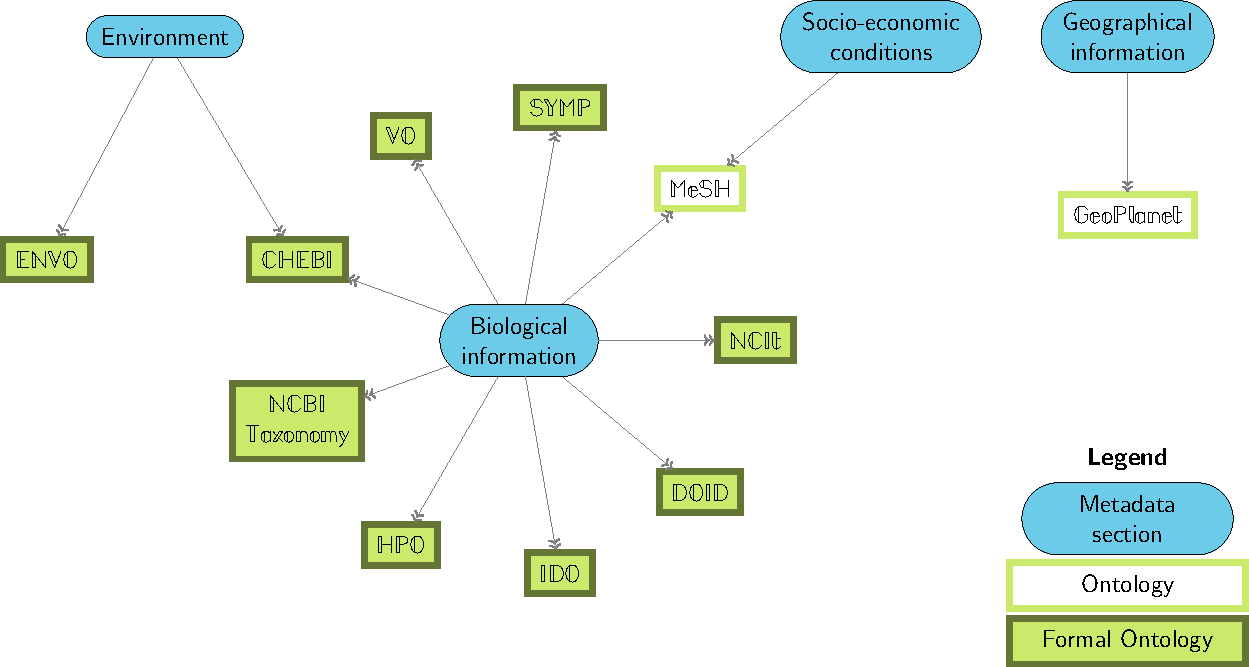
\includegraphics[width=0.9\textwidth]{images/nero.pdf}
    \caption[The Network of Epidemiology-Related Ontologies]{This figure represents NERO as a set of metadata sections (represented as blue round rectangles) and the ontologies used to annotate the epidemiology resources (in straight rectangles). Each metadata section is associated with a set of ontologies that contain the concepts relevant for that section. There is a difference between formal ontologies (represented with the shaded green background) and the other vocabularies, as explained in the last paragraph of \appref{app:ontologies}.}
    \label{fig:nero}
\end{figure}

To maximise the benefits of using ontologies, I contributed to the establishment of the Network of Epidemiology-Related Ontologies (NERO). This is a multi-domain collection of ontologies that represent parts of the epidemiology field: \eg diseases, symptoms, chemical compounds, modes of transmission, \etc. It also contain non-biomedical ontologies to represent demography, environmental conditions, geographical regions and socio-economic conditions. NERO was integrated in the Epidemic Marketplace as a way to facilitate annotation of resources, by suggesting concepts based on the content of the resource and facilitating the annotation process with an auto-complete-like feature that suggested concepts from those ontologies. As such, NERO bridges the gap between automatic systems and epidemiology, a domain which traditionally makes poor use of computer power (possibly because of its high heterogeneity), by bringing the semantic web into it. In fact, prior to NERO, there was not an expressive way to annotate resources with ontology concepts in this field. \figref{fig:nero} contains a graphical representation of which ontologies are used to fill the metadata model for an epidemiology resource.


\section{Text-mining} \label{sec:auxiliary-projects/text-mining}

Text-mining aims at extracting relevant information from unstructured natural text. The meaning of ``relevant'' depends on the actual goals of the text-mining process: for example, automatic news processing systems can perform ``Sentiment analysis'', a technique that detects whether the opinions expressed in text (in a full article, a blog post, a tweet, \etc.)\ is positive or negative; advanced algorithms can even classify text based on more specific emotional states, such as ``angry'', ``sad'' or ``happy''. In the biomedical domain, text mining is an important part of scientific discovery: it can be used to find drug targets and biomarkers, for drug repositioning, to create a clinical overview of a certain therapeutic area, to create domain specific databases, \etc.~\citep{Fleuren2015}.

The first preliminary study I was part of, in the context of text mining, was the application of semantic similarity to disambiguate geographical names in news articles~\citep{Batista2012}. Names of geographical features (called ``toponyms'') are particularly ambiguous: a particular case is in the name \emph{Lisboa}, which represents up to $41$~different locations in the territory of Portugal alone, from streets to a municipality, a city and a region. Being able to properly identify which place is being referred to in text is important to further process that text. One way to achieve this is by:
\begin{enumerate}
    \item associating each toponym with a set of its possible locations;
    \item comparing all the locations within each possible arrangement using semantic similarity;
    \item finding the arrangement with highest overall similarity score and choose it as the disambiguated set of locations.
\end{enumerate}

In this work, we used Geo-Net-PT, a geographical ontology of the Portuguese territory, which contains more than $400{,}000$ geographical locations, organised in a hierarchy (\eg \term{Portugal} \prop{contains} \term{Lisbon city}). This hierarchy can be used to compute semantic similarity with the algorithms mentioned in the main document, thus allowing the disambiguation process above.

I have also contributed to text-mining approaches in the biomedical domain. One of the most important tasks in text processing in biomedical informatics is the identification of entities such as chemical compounds in text. This allows further processing (for example, the detection of interaction between compounds). I have worked as a semantic similarity expert with a set of colleagues in text-mining in this context. In a first step, we investigated whether semantic similarity can be used to disambiguate chemical names in text, just like I had done previously in the geographical domain~\citep{Lamurias2015}. In a second step, we investigated whether semantic similarity can also be used to improve the overall performance a system designed to find interactions between two chemical compounds in text~\citep{Lamurias2014}. For example, the sentence ``\emph{Trilostane} may interact with \emph{aminoglutethimide}, causing too great a decrease in adrenal function'' describes the interaction between two compounds (in slanted text), which the system is able to find. Semantic similarity was used here in an effort to reduce false positive interactions found by the system.


\section{Ontology alignment} \label{sec:auxiliary-projects/alignment}

Part of my research in multiple-ontology semantic similarity was dedicated to the study of ontology alignment techniques. As explained throughout this document, multi-ontology semantic similarity is enhanced if the ontologies used to compute similarity are related to each other in some way. In general ontology alignment is done by asserting that two concepts from different ontologies are equivalent. In the context of multiple-ontology single-domain measures (see \secref{sec:sota/multi-ontology}), complementary ontologies improve the accuracy of similarity only if the ontologies are \emph{linked}.

\begin{figure}
    \centering
    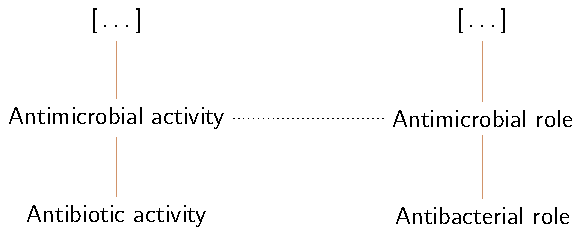
\includegraphics{images/alignment.pdf}
    \caption[Partial alignment between two ontologies of the biochemical domain]{The two ontologies partially illustrated here represent the same domain of reality, namely the roles of biochemical molecules. The dotted line represents an \emph{equivalence} link between the two, and can be explored by multiple-ontology semantic similarity to compare concepts in different ontologies.}
    \label{fig:simple-match}
\end{figure}

For example, with the aligned pair of ontologies in \figref{fig:simple-match}, it would be possible to assign a relatively high value to the similarity between \term{Antibiotic activity} and \term{Antibacterial role}, but only if their parent concepts (\term{Antimicrobial activity} and \term{Antimicrobial role} respectively) are explicitly marked as \emph{equivalent}, as the dotted line suggests.

The set of equivalences between multiple ontologies (called an \emph{alignment}) is, therefore, essential to single-domain multiple-ontology similarity measures. However, finding them is labour-intensive, given the amount of concepts in biomedical ontologies, which has lead the community to develop ``ontology matching'' algorithms, which find, automatically or semi-automatically, equivalent concepts within two or more ontologies~\citep{Euzenat2007}. Ontology alignments can be made with simple textual matching, which rely on dictionaries and thesauri to increase their recall (for instance, the fact that ``activity'' and ``role'' are synonyms might be used to match the two concepts in the ontologies from \figref{fig:simple-match}); they can also leverage on the structure of the ontologies to find related concepts (concepts with many linked subclasses should themselves be linked); and they can also explore the logical definitions on the ontologies to find these matches~\citep{Shvaiko2005}.

During the early stages of my PhD, I worked under the assumption that ontology alignment would be essential for my research. As such, I participated in Semantic Ontology Matching using External Resources (SOMER), a project funded by the Fundação para a Ciência e Tecnologia (the Portuguese Foundation for Science and Technology), and which ran from 2012 to~2014. One of the tasks that I developed was the alignment of geographical ontologies (namely the Yahoo!~GeoPlanet, a geography ontology for world-wide locations, and the Geo-Net-PT, mentioned above).

As it turns out, ontologies that represent different domains of the biomedical information are usually already quite orthogonal, given the OBO Foundry's principles and the best practices in ontology development (see \appref{app:ontologies}) and, therefore, this technique is not vital for the calculation of similarity among concepts from different ontologies. As such, the total effort that I put into this project, with regard to my PhD, was relatively small when compared to other endeavours, since I recognised that the outputs of the project would not benefit multi-domain semantic similarity to a large extent.



\small
\printbibliography

\end{document}
